\documentclass[12pt]{article}
\usepackage{amssymb,amsthm,amsmath,setspace,paralist}
\usepackage{url}
\usepackage[usenames,dvipsnames]{color}
\usepackage{lineno}
%\usepackage[labelfont=bf,format=hang,textfont=it]{caption}
\usepackage{graphicx}
\usepackage{microtype}
\usepackage[letterpaper,text={15cm,23cm}]{geometry}
\usepackage{natbib}
\usepackage{hyperref}
\usepackage{subfig}

\bibliographystyle{gcb} 

%% for internal use
\newcommand{\fixme}[1]{\emph{\marginpar{FIXME} (#1)}}
\newcommand{\readme}[1]{\emph{\marginpar{README} (#1)}}

\newcommand{\degree}{\ensuremath{^\circ}}

\definecolor{Red}{rgb}{0.5,0,0}
\definecolor{Blue}{rgb}{0,0,0.5}
\hypersetup{%
  pdftitle = {Near real-time disturbance detection in terrestrial ecosystems using satellite image time series: Drought detection in Somalia},
  pdfsubject = {remote sensing, monitoring},
  pdfkeywords = {early warning, real-time monitoring, global change, disturbance, time series, remote sensing, vegetation and climate dynamics},
  pdfauthor = {Jan Verbesselt, Achim Zeileis, Martin Herold},
  %% change colorlinks to false for pretty printing
  colorlinks = {true},
  linkcolor = {Blue},
  citecolor = {Blue},
  urlcolor = {Red},
  hyperindex = {true},
  linktocpage = {true},
}

\begin{document}

\linenumbers
%\modulolinenumbers[5]

\title
    {
    Near real-time disturbance detection in terrestrial ecosystems using satellite image time series: \\ Drought detection in Somalia
    }

\author{Jan Verbesselt\thanks{Corresponding author. \emph{Ph}: + 31 317 48 52 68; \emph{Fax}: +31 317 419000;
        E-mail: \url{Jan.Verbesselt@wur.nl}} $^{1}$, 
        Achim Zeileis$^2$, Martin Herold$^1$
}
\maketitle

\footnotetext[1]{Remote sensing team, Wageningen University,
            Droevendaalsesteeg 3, Wageningen 6708 PB, The Netherlands}
\footnotetext[2]{Department of Statistics, Universit\"at Innsbruck,
            Universit\"atsstr.~15, A-6020 Innsbruck, Austria}

\doublespacing
%\singlespace
%http://www.fao.org/giews/pricetool2/
\begin{abstract}

Near real-time monitoring of ecosystem disturbances is critical for addressing impacts on carbon dynamics, biodiversity, and socio-ecological processes. Satellite remote sensing enables cost-effective and accurate monitoring at frequent time steps over large areas. Yet, generic methods to detect disturbances within newly captured satellite images are lacking. 
We propose a generic time series based disturbance detection approach by modelling \emph{stable} historical behaviour to enable detection of \emph{abnormal} changes within newly acquired data.
Time series of vegetation greenness provide a measure for terrestrial vegetation productivity over the last decades covering the whole world and contain essential information related land cover dynamics and disturbances. Here, we assess and demonstrate the method by (1)~simulating time series of vegetation greenness data from satellite data with different amount of noise, seasonality and disturbances representing a wide range of terrestrial ecosystems, (2)~applying it to real satellite greenness image time series between February 2000 and July 2011 covering Somalia to  detect drought related vegetation disturbances.
First, simulation results illustrate that disturbances are successfully detected in near real-time while being robust for seasonality and noise. Second, major drought related disturbance corresponding with most drought stressed regions in Somalia are detected from mid 2010 onwards and confirm proof-of-concept of the method. The method can be integrated within current operational early warning systems and has the potential to detect a wide variety of disturbances (e.g.\ deforestation, flood damage, etc.). It can analyse in-situ or satellite data time series of biophysical indicators from local to global scale since it is fast, does not depend on thresholds or definitions and does not require time series gap filling. 

%% remove 20 words!!!!
%Further work is needed for operational implementation of the method to enable a rapid response by applying it to time series data with a high temporal resolution (e.g., hourly or daily data).
%\textbf{Research Highlights}
%\begin{itemize}
%    \item A novel near real-time time series based change detection approach.
%    \item Validation by simulating time series and applying it on real satellite data
%    \item Proof-of-concept illustrated for severe drought currently affecting Somalia
%    \item The approach is robust, fast, and flexible to different data sets and does not require gap filling or smoothing.
%    \item The is freely available as a function in the \emph{bfast} package for the open-source statistics system {R}.
%\end{itemize}

\medskip

\noindent\emph{Key words:}\quad
Early warning, real-time monitoring, global change, disturbance, time series, remote sensing, vegetation and climate dynamics

\end{abstract}

\newpage

\section{Introduction}

Real-time ecosystem disturbance detection is critical for tracking human-induced and natural disturbances promptly \citep{Asner:2011fa}. Such
information is needed for signalling abnormal developments, quickly raising awareness and reducing negative impacts to natural resources, humans, and infrastructure. Ecosystem disturbances can also contribute to the current rise of carbon dioxide ($CO_2$) levels in the atmosphere due to the emission of $CO_2$ from terrestrial biomass loss \citep{Potter2003,Schimel:2001vi}. 
Key to approaches looking at disturbances is that many recent change events occur worldwide at unknown locations. In this sense, remote sensing tools can be in the first instance used to alert when things start to appear \emph{abnormal}. For example, deviations from \emph{normal} land surface phenology, defined as the seasonal variation in vegetated land surface from satellite sensors \citep{White2009}, can indicate deforestation activities \citep{Asner:2011fa}, forest health issues (e.g.\ tree mortality) \citep{Hargrove2009, Stone2008, Verbesselt2009}, drought and climate anomalies \citep{Funk:2009vf,Vrieling:2011da}.

% satellite data and vegetation indices
Satellite sensors are well-suited to provide consistent and frequent measurements over large areas which is appropriate for capturing the effects of many processes that cause disturbances, including physical (e.g.\ droughts, fires, floods), biogenic (e.g.\ herbivorous insects and pathogens) and anthropogenic (e.g.\ deforestation, urbanisation, farming) disturbances \citep{Jin2005, Potter2003}. A common way to derive indicators of ecosystem dynamics and disturbances is the use of spectral vegetation indices such as the Normalised Difference Vegetation Index (NDVI) related to the photosynthetic capacity of vegetation canopies \citep{Myneni1995, Pettorelli:2005ed, Potter2003}.  Although NDVI might be affected by soil background and a saturation effect at high biomass levels, it captures seasonal and inter-annual changes in vegetation status \citep{Huete2002,Myneni:1997ur}.% fraction of photosynthetic active radiation (wavelength 0.4--0.7 $\mu m$)

% different change types in ecosystem dynamics
The ecosystem changes commonly observed with remote sensing approaches can be divided into three categories: (1)~\emph{seasonal or cyclic change}, driven by annual temperature and rainfall interactions impacting plant phenology resulting in distinct intra-annual patterns for different vegetation types; (2)~\emph{gradual trend change} such as trends in mean annual rainfall or gradual change in land management (e.g., long term drought, forest regrowth after fire) that result in changes over several years; and (3)~\emph{abrupt trend change}, caused by events from human activities (e.g., deforestation) or natural causes (e.g., wind throw or an extreme drought event) that change land cover over short time frames (days or weeks) 
\citep{Beurs2005a,Verbesselt2009a,Verbesselt:2010wo}. 

% problem statement
Detecting changes within time series is the first step towards understanding the acting processes and drivers (e.g.\ natural or anthropogenic). Estimating change from remotely sensed data series however is not straightforward, since time series contain a combination of seasonal, gradual and abrupt ecosystem changes occurring in parallel, in addition to noise that originates from the sensing environment (e.g., view angle), remnant geometric errors, atmospheric scatter and cloud effects \citep{Beurs2005a, Roy2002, Wolfe1998}. The ability of any system to detect change depends on its capacity to differentiate normal phenological cycle from abnormal change (e.g., drought anomalies, degradation, deforestation). 
Several change detection methods are available to detect disturbances within historical satellite image time series \citep{deBeurs:2005jq, Verbesselt2009a, Verbesselt:2010wo, White2006} but generic methods to detect disturbances within newly captured satellite images are lacking. Three major challenges remain.

% changes at the end of a time series -(what is normal and what is abnormal can maybe be mentioned above?)
First, it is crucial to be able to detect disturbances within newly captured satellite images to enable a rapid response or early warning. In previous work, we proposed an approach,  BFAST i.e.\ Break detection For Additive Season and Trend, for change detection within seasonal time series \citep{deJong:wo, Verbesselt2009a,Verbesselt:2010wo}.
BFAST detects and characterises trend and seasonal changes within historical time series but the method is not developed to detect disturbances in recently
acquired data. Methods to detect changes in near real-time, also referred to as monitoring techniques, have been suggested in the statistics and
econometrics literature to assess the stability of linear regression models \citep{Chu1996}, e.g., for investigating exchange rate dynamics
\citep{Zeileis:2010tt}. However, these methods have not been optimised for real-time disturbance detection of terrestrial ecosystems using remotely sensed time series data.

% threshold independent
Second, change detection techniques for global disturbance monitoring need to be independent of vegetation-specific thresholds while being robust against the inherent noise and seasonality captured within time series.
Most change detection methods require user designation of a threshold or change type definition separating real change from spectral changes caused by variability in illumination, seasonality, or atmospheric scattering \citep{Lu2004, Potter2003, Hayes2007}.  \citet{White2006} presented a method for real-time monitoring but requires a region-specific threshold for detecting change. The determination of thresholds adds significant cost to efforts expanding change detection across regions or becomes complex when the regions are changing. A historical analysis using archived satellite data is needed to model normal, expected behaviour against which abnormal behaviour, i.e.\ disturbance, in the near future can be described \citep{Hargrove2009}. There is a critical need to enable analysis of time series independent of specific thresholds or definitions to detect disturbances.

% missing data: avoid smoothing and interpolation
Third, change detection methods need to deal with missing data (e.g., clouds or sensor defects) in time series data.
Existing change detection methods smooth or fill gaps \citep{Jonsson2002, Roerink2000, Julien2010} when dealing with noisy times series of remotely sensed data. For a given date, these methods typically require looking both backwards and forwards in time, negating use in real-time or forecast applications \citep{White2006}.  Furthermore, gap filling techniques model data based on assumptions of normal data variation which inhibits the detection of disturbances \citep{Samanta:2011hp}. Hence, methods able to analyse and detect changes in non-gap-filled time series are urgently needed for global change monitoring.

We propose a multi-purpose approach for near real-time disturbance detection using time series data that does not require specific thresholds and deals with missing data. The following major research questions are answered in this paper: \\
(1)~Can a period, representing stable (i.e.\ normal) historical data variation representing both seasonal and gradual changes, be identified within a time series?\\
(2)~Is the model representing the \emph{normal} historical data variation able to reliably and quickly differentiate between normal and \emph{abnormal} changes (i.e.\ disturbances) within newly incoming observations (i.e., near real-time)?

We assess this approach for different ecosystems by simulating NDVI time series with varying amounts of seasonal variation and noise, and by adding changes with different magnitudes representing a wide variety of terrestrial ecosystems.  We demonstrate the proof-of-concept using the MODIS (Moderate Resolution Imaging Spectrometer) NDVI 16-day image composites from February 2000 until July 2011 for drought disturbance detection in Somalia. NDVI time series are also used by organisations like the European Research Centre (JRC), the United State's Warning System Network (FEWS-NET), and the United Nations Food and Agricultural Organisation (FAO) as an early warning of potential food production problems in African countries \citep{Rojas:2005bz}.
 
\section{Material and methods}

\subsection{Real-time disturbance detection}\label{sec:Method}

When investigating disturbances using satellite data, many approaches \citep[e.g.,][]{deJong:wo,Potter2003, Verbesselt:2010wo, White2009} focus on the question if and where disturbances occur in the season and trend component of a given observed time series $t = 1, \dots, n$. Here, we want to investigate a different question: \emph{Do new observations $t = n, n + 1, \dots$ still conform with the expected behaviour of the historical sample $t = 1, \dots, n$}~? Thus, we want to detect disturbances at the end of a time series by comparison with representative, i.e.\ stable, historical observations. Here, a method is presented that is able to detect disturbances within newly acquired time series data by automatically identifying a stable history period (Section~\ref{sec:StableHist}) to model normal expected behaviour (Section~\ref{sec:seasontrendmodel}) against which disturbances can be detected (Section~\ref{sec:MonStrucChange}).

Validation of multi-temporal change-detection methods is often not straightforward, since independent reference sources for a broad range of potential changes must be available \citep{Kennedy2007}. Thus, we simulated 16-day NDVI time series with different noise levels, seasonality, and disturbances in order to robustly test the disturbance detection approach in a controlled environment \citep{Verbesselt2009a, Verbesselt:2010wo}. It, however, is challenging to create simulated time series that approximate remotely sensed time series, because these contain combined information on vegetation phenology, inter-annual climate variability, disturbance events, sensor conditions (e.g., viewing angle), and signal contamination (e.g. clouds) \citep{Zhang2009}. Hence, we tested the method by (1)~a simulation experiment (Section~\ref{sec:Valsim}) and (2)~analysis of 16-day MODIS satellite NDVI time series for drought disturbance detection Somalia (Section~\ref{sec:RealData}). 

%The methods proposed here are based on a similar additive season and trend
%model as employed by \citet{Verbesselt:2010wo}. However, while
%\citet{Verbesselt:2010wo} focussed on the question if and where structural breaks occur in the season and trend component of a given observed time series
%$t = 1, \dots, n$, we want to investigate a different question:
%\emph{Does the season-trend model for future observations $t = n, n + 1, \dots$ still
%conform with the season-trend model established for the historical sample
%$t = 1, \dots, n$}~? Thus, we want to monitor potential abnormality at the end of a time series, in
%real-time, by comparing it with historical observations.

\subsection{Season-trend model}\label{sec:seasontrendmodel}

The method proposed here is based on a similar additive season and trend model as employed by \citet{Verbesselt:2010wo} to account seasonal and trend changes typically occurring within climate driven biophysical indicators derived from satellite data (e.g.\ NDVI)  \citep{Beurs2005a}. For the observations $y_t$ at time $t$, a season-trend model is assumed with linear trend and harmonic season:
%
\begin{eqnarray} \label{eq:lmod}
  y_t & = & \alpha_1 + \alpha_2 t + \sum_{j = 1}^k \gamma_{j} \sin \left(\frac{2\pi j t}{f} + \delta_{j} \right) ~+~ \varepsilon_t,
\end{eqnarray}
%
where the intercept $\alpha_1$, slope $\alpha_2$ (i.e., trend), amplitudes $\gamma_1, \dots, \gamma_k$,
and phases $\delta_1, \dots, \delta_k$ (i.e., season) are the unknown parameters,
$f$ is the known frequency (e.g., $f = 23$ annual observations for a 16-day time series),
and $\varepsilon_t$ is the unobservable error term at time $t$ (with standard deviation $\sigma$). In the applications
below, we employ three harmonic terms (i.e., $k = 3$) to robustly detect disturbances within MODIS NDVI time series, as components four and higher represent variations
that occur on a three-month cycle or less \citep{Geerken2009,Julien2010}. The model (Eq.~\ref{eq:lmod}) can be written as standard a linear regression model \citep[see e.g.,][Chapter~3.3]{Cryer2008}:
%
\begin{eqnarray*} \label{eq:OLSlmod}
  y_t   & = & x_t^\top \beta ~+~ \varepsilon_t, \\
  x_t   & = & \left\{1, t, \sin(2 \pi 1 t / f), \cos(2 \pi 1 t / f),
              \dots, \sin(2 \pi k t / f), \cos(2 \pi k t / f)\right\}^\top, \\
  \beta & = & \left\{\alpha_1, \alpha_2, \gamma_1 \cos(\delta_1), \gamma_1 \sin(\delta_1),
              \dots, \gamma_k \cos(\delta_k), \gamma_k \sin(\delta_k)\right\}^\top,
\end{eqnarray*}
%
containing the $p = 2 + 2 k$ regression parameters $\beta$ which can be estimated and tested using ordinary least squares (OLS) techniques. 
If there are gaps in the time series $y_t$, these observations are simply omitted prior to estimation of $\beta$ which can then still consistently 
be identified (unless \emph{all} observations at certain frequencies are missing). The season-trend model takes the underlying trend and seasonal variation within a time series into account so that season-trend patterns are removed in the resulting residuals. This corresponds to approaches where in multiple steps a time series is `detrended' and `deseasonalized' \citep{Potter2003} whereas here the adjustment is done in a single step by OLS-fitting of the season-trend model.

\subsection{Monitoring structural change}\label{sec:MonStrucChange}

Based on the season-trend model introduced above, the question raised in
the introduction can be rephrased: \emph{Given that a stable season-trend model was estimated in an observed
time period, does it remain stable for new observations?} A disturbance is detected when the model does not remain stable for new incoming observations.
As the season-trend model can be formulated as an OLS regression,
we can leverage methods proposed in the structural change literature
for linear regression models where this problem is known as \emph{monitoring}
of structural changes \citep{Chu1996}.
The idea for monitoring techniques is simple. Given that the parameters
$\beta$ can be consistently estimated as $\hat \beta$ from a stable history
period $t = 1, \dots, n$, we want to check whether $\hat \beta$ still fits
the data $y_t$ for $t > n$ (i.e.\ for new data). To do so, some measure of discrepancy is needed \citep[][]{Chu1996, Leisch2000, Zeileis2005a}. Here, we use moving sums (MOSUMs) of the residuals in the monitoring
period $t = n + 1, \dots, N$:
%
\begin{eqnarray}
  MO_t & = & \frac{1}{\hat \sigma \sqrt{n}} \sum_{s = t - h + 1}^t (y_s - x_s^\top \hat \beta),
\end{eqnarray}
%
where $h$ is the bandwidth of the MOSUM and is typically chosen relative to
the size of the history sample, e.g., $h = n/4$ or $h = n$ \citep{Zeileis2005a, Zeileis:2010tt}.
If the model remains stable, the MOSUM process $MO_t$ should be close to zero and
fluctuate only randomly. However, if a structural change occurs, $MO_t$ will deviate
systematically from zero. A structural break is declared if the absolute value
$|MO_t|$ exceeds some boundary that is asymptotically only crossed with 5\%
probability under structural stability. 
If there are missing values in $y_t$ in the monitoring period, these are 
again simply not included in the MOSUM $MO_t$, i.e.\ only reduce the number 
of observations available. The technical details for the boundary are based
on a so called functional central limit theorem \citep[see][for details]{Leisch2000}.
The boundary function employed here is taken from \citet[Eq.~7]{Zeileis2005b}.

% Here, we use the boundary function $c \sqrt{2 \log_+ t/n}$, where $\log_+ x$ is $1$ for $x \le e$ and $\log x$ otherwise and $c$ is the critical value that determines the significance level. The critical values also depends on the choice of $h$ and the monitoring horizon $N$, e.g., for $h = 0.25 n$ and $N = 10 n$, $c = 1.3409$ at the 5\% level.

\subsection{Selecting the stable history period}\label{sec:StableHist}

A crucial assumption for the monitoring approach proposed above is that
the history period $t = 1, \dots, n$ itself is free of disturbances, that the parameters $\beta$ are stable during this time, and can be used to model normal expected behaviour. In practice, there are often long series of observations $y_t$ available
before the start of the monitoring process and it would be naive to assume
that always all of these observations can be adequately captured by a single
season-trend model. Hence, a natural idea is to not use all observations
but only the last $l, \dots, n$ observations with $l \ge 1$ so that a stable
season-trend model can be fitted. 
Here, we implement a technique proposed by \citet{Pesaran2002} that by moving backward in time for $t = n, n-1, n-2, \dots$ considers a cumulative prediction error until the season-trend model (Eq.~\ref{eq:lmod}) breaks down. The method is also known as reversed-ordered-cumulative sum (CUSUM) of residuals, or ROC.
The CUSUM test \citep[see][for more details]{Zeileis2002} is based on similar ideas as the monitoring approach introduced
above and the ROC method simply applies it in reverse ordering.

Fig.~\ref{fig:SimMonitor} provides an overview of the three steps that are being performed when applying the real-time disturbance detection approach. 
Two periods are defined within a time series; (a)~a \emph{history period} i.e., data that already has been acquired and which will be analysed for stability
in order to model normal vegetation dynamics, and (b)~a \emph{monitoring period} i.e., the period representing new data that recently has been captured that
needs to be analysed for disturbances. The blue line illustrates the fit of the season-trend model on the identified stable part of the history period of an
example NDVI time series (Section~\ref{sec:seasontrendmodel} and~\ref{sec:StableHist}). This season-trend fit is used to model the normal expected behaviour
in the \emph{history period} and as such detect abnormal data variations, disturbances, within the \emph{monitoring period}
(Section~\ref{sec:MonStrucChange}). Here, a disturbance is detected with only a short delay.

%In summary, when applying the real-time disturbance approach three steps are being performed: (1)~verify which part of the history period is stable (Section~\ref{sec:StableHist}), (2)~fit the season-trend model on the stable history period (Section~\ref{sec:seasontrendmodel}) and (3) assess whether the stable history model is still valid for the new incoming data (Section~\ref{sec:MonStrucChange}, i.e.\ disturbance detection).

%\section{Validation}\label{sec:Validation}

\subsection{Simulation experiment}\label{sec:Valsim}

The objective of the time series simulation experiment is to assess the \emph{detection delay}, i.e.\ how much new data is required to detect a disturbance,
while varying the amount of noise, seasonal amplitude, and the magnitude of the disturbance in the simulated time series. NDVI time series were simulated
using a similar approach as proposed by  \citet{Verbesselt:2010wo} representing a wide range of ecosystem dynamics. Simulated NDVI time series are generated by summing individually simulated season, trend, and noise components (Fig.~\ref{fig:SimMonitor}). 

First, the seasonal component is created using an asymmetric Gaussian function with an amplitude ($a$) for each season. Second, a disturbance was added to the trend component (e.g., fire or drought) by combining a step function with a magnitude ($m$) and fixed gradient recovery phase. Third, the noise component was generated using a random number generator that follows a normal distribution N($\mu = 0$, $\sigma =x$). Vegetation index specific noise was generated by randomly replacing the white noise by noise with a value of $-0.1$, representing cloud contamination that often remains after atmospheric correction and cloud masking procedures \citep[see][for more details]{Verbesselt:2010wo}. Fig.~\ref{fig:SimMonitor} shows a simulated 16-day MODIS NDVI time series with $a = 0.2$, $\sigma = 0.05$, containing one simulated abrupt change with $m = -0.3$.

In the simulation experiment the \emph{history period} is defined as the period from 2000 until mid 2006 (i.e., the time step just before the simulated break), whereas the \emph{monitoring period} is defined as the period from the simulated break onwards of which the length is gradually increased during the experiment ($d$) (Fig.~\ref{fig:SimMonitor} and Table~\ref{table:simpar}). We selected a range of $a$, $\sigma$, and $m$ values for the simulation study to represent a large range of land cover types of different data quality while varying the amount of data, $d$, available in the monitoring period (Table~\ref{table:simpar}). An example of the set-up of the simulation experiment is shown in Fig.~\ref{fig:SimMonitor}. 1000 iterations of all the combinations of $\sigma$, $a$, $d$ and $m$ were performed to quantify the probability of detecting a disturbance in the monitoring period in relation to the amount of data available ($d$).

%Two periods are defined within the simulated time series to validate the real-time monitoring approach; (a)~a \emph{history period} i.e., data that already has been acquired and which will be analysed for stability in order to model normal vegetation dynamics, and (b)~a \emph{monitoring period} i.e., the period representing new data that recently has been captured that needs to be analysed for disturbances. 

\subsection{Drought disturbance detection in Somalia}\label{sec:RealData}

The use of the real-time monitoring approach is demonstrated using the 16-day MODIS NDVI composites with a 0.05\degree \ spatial resolution (MOD13C1 collection~5). This product provides  NDVI corrected for the effect of atmospheric gases, thin cirrus clouds and aerosols as a proxy for global scale vegetation dynamics and disturbances \citep{Huete2002}.
The MOD13C1 global satellite images were acquired from February 2000 to July 2011 and were analysed for disturbances from mid 2010 onwards covering Somalia
in order to assess the impact of the 2010--2011 drought on the vegetation photosynthetic capacity. The MODIS quality assurance (QA) flags are used to select
only cloud-free data of optimal quality. An NDVI time series is only analysed when either (1)~it lacked less than 15\% of observations masked out by the QA
flags and (2)~covering vegetated land; i.e.\ having a median of NDVI time series larger than 0.2 NDVI \citep{Beurs2009, deJong:wo, Vrieling:2011da}. The
noise level ($\sigma$) of NDVI time series is estimated by deriving the standard deviation of the residuals from the fitted season-trend model
(Eq.~\ref{eq:lmod}) on the stable history period.  The magnitude and direction of the disturbance is estimated by deriving the difference between the median
of the fitted season-trend model and the new observations during the monitoring period.

Somalia has a tropical but not torrid climate, and there is little seasonal change in temperature. In the low areas, the mean temperature ranges from about 24\degree~C to 31\degree~C. The plateau region is cooler, the southwest warmer. The periodic winds, the southwest monsoon (June--September), and the northeast monsoon (December--March) influence temperature and rainfall. Rain falls in two seasons of the year: heavy rains from March to May, and light rains from September to December. Average annual rainfall is estimated at less than 28 cm (\url{www.nationsencyclopedia.com}).  However, after a period of persistent poor rains during the past decade, the autumn 2010 rains were poor and the spring rains in 2011 failed completely \citep{Funk:2011fg}. The lack of rainfall combined with high food prices has weakened the population's resilience to food emergencies and are among most important factors explaining the severe and ongoing famine in Somalia today. The monthly rainfall anomaly time series shown in Fig.~\ref{fig:RF} illustrates the lack of rainfall in the last decade and the severity of the rainfall anomaly occurring from mid 2010 onwards in Southern Somalia. The spatial extent of the drought severity is illustrated by the February--March 2011 rainfall \citep{Xie:1997tw} and land surface temperature anomaly for Somalia (Fig.~\ref{fig:RF_LSTSomalia}). Below normal rainfall and above normal temperatures occurred during February--March 2011 in south Somalia.


%  Read more: Climate - Somalia - average, annual, temperature http://www.nationsencyclopedia.com/Africa/Somalia-CLIMATE.html
%Most of the country receives less than 500 millimeters of rain annually, and a large area encompassing the northeast and much of northern Somalia receives as little as 50 to 150 millimeters. Certain higher areas in the north, however, record more than 500 millimeters a year, as do some coastal sites. The southwest receives 330 to 500 millimeters. http://www.climate-zone.com/climate/somalia/

% http://www.fao.org/giews/pricetool2/  % we can add a time series of the food prices to illustrate the problem
% 

\section{Results}

\subsection{Simulation experiment} \label{sec:DiscSim}

Fig.~\ref{fig:SimNr} illustrates the probability for detecting a break within the monitoring period of a time series while varying the noise level ($\sigma$), magnitude of simulated disturbance ($m$) and the amount of data available in the monitoring period ($d$). The seasonal amplitude ($a$) did not influence the probability for break detection and results shown in Fig.~\ref{fig:SimNr}  are valid for the different simulated $a$'s (Table~\ref{table:simpar}). 
Random and NDVI specific noise levels were introduced to simulate disturbances in the history period of the simulated time series and trigger identification of stable history periods with different lengths. The length of the identified stable history period also did not influence the probability for break detection (results not shown). We, however, recommend limiting the disturbance detection to time series with a stable history period longer than 2 years (i.e.\ 46 observations representing two seasons in this study) to enable a reliable estimation of the 8~season-trend model parameters. Furthermore, Fig.~\ref{fig:SimNr} shows that a break with $m = -0.4$ can be detected when $\sigma$ is smaller than 0.1 and $d < 3$.  When the magnitude of
the break is larger (e.g., $m = -0.6$), less observations ($d<4$) are required for a similar amount of noise (e.g., $\sigma < 0.1$). 
% what is not tested here is that when a disturbance occurs later in the monitoring period the probability to detect disturbance is influenced...
% the delay time for disturbance detection is important!!! (how fast can a change be detected?)
% to do search for a forest in Somalia - i.e.\ high median NDVI - in order to illustrate this concept - when can also illustrate this for a pixel modis MOD13C1 for a fire in Victoria (coordinates -> query from the database - and plot an example).

\subsection{Drought disturbance detection in Somalia} \label{sec:DiscReal}

We demonstrate the proof-of-concept of a multi-purpose near real-time disturbance detection method by analysing MODIS 16-day NDVI image time series. Here, the disturbance detection is limited to areas (1)~with a minimum amount of vegetation cover by restricting the analysis to time series with a median NDVI $>0.2$ during the 2000--2011 period \citep{Vrieling:2011da} and (2)~with a stable history longer than two years (see Section~\ref{sec:DiscSim});

\begin{enumerate}[(1)]

\item Fig.~\ref{fig:spatiala} illustrates the median of an NDVI image time series (2000--2011) as a proxy for vegetation cover during the period of
analysis. Areas with no or very low vegetation cover are occurring in the North East of Somalia whereas areas with higher vegetation cover are situated in
the South of Somalia. Similar approaches have been used by \citet{Brown:2010fq} and \citet{Vrieling:2011da} to study response of African land surface
phenology. The NDVI time series with no or very low NDVI values do not show any seasonal climate related vegetation dynamics and are mainly influenced by
irregular variations of the soil background. The areas with NDVI values above 0.2 correspond to the areas where below normal rainfall and above normal land
surface temperature is occurring (Fig.~\ref{fig:RF_LSTSomalia}) which illustrates that a severe drought is impacting areas with a minimum amount of vegetation cover (NDVI~$> 0.2$). 

\item Fig.~\ref{fig:spatialb} illustrates the spatial variation of the length of the stable history period and is used to restrict the analysis to regions
with a stable history longer than 2 years. The stable history is identified for modelling normal variation within the history period to enable
differentiation from abnormal changes, i.e.\ disturbances, in the monitoring period (i.e.\ mid 2010 onwards). The ROC approach (Section~\ref{sec:StableHist})
verifies whether or not a structural change is occurring while stepwise going back in history. The length of the stable history (Fig.~\ref{fig:spatialb})
can be used as an approximation of the occurrence of the most recent large (enough) disturbance in the history period. (If a more precise estimate of the
timing of this last major disturbance if of interest, more appropriate methods are available, e.g.\ \citealp{Bai2003}, or \citealp{Verbesselt2009a}.) Analysed NDVI time series for specific locations are shown in Fig.~\ref{fig:realmon} where for time series in Fig.~\ref{fig:realmon}a and c the whole history period and in Fig.~\ref{fig:realmon}b a shorter stable history period is identified as stable. The short history period in Fig.~\ref{fig:realmon}b can be explained by a lack of rainfall at the beginning of 2008 \citep{Funk:2009vf}. 

%\readme{Double check the detection delay discussion}
%The BFAST approach is developed to accurately estimate time, magnitude, and direction of change within historical time series but it is not developed to detect disturbances in new observations (i.e.\ near real-time monitoring) . 
%The method for identifying the stable history is based on the structural change detection methods \citep{Zeileis:2010tt} and is implemented to assess stability of the history period. 

\end{enumerate}

Fig.~\ref{fig:spatialc} shows the spatial variation of the noise level (i.e.\ $\hat \sigma$ of the residuals of the season-trend model) where low $\hat
\sigma$ correspond to the low vegetated areas and the high $\hat \sigma$ correspond to the semi-arid ecosystems (e.g.\ woodland and savannah) (see
Fig.~\ref{fig:spatiala}). High $\hat \sigma$  in the semi-arid ecosystems can be explained by large inter-annual phenological shifts (e.g.\ shifts in the
start and end of the growing season) and double growing seasons when compared to areas with low vegetation cover or forested areas \citep{Verbesselt:2010wo,
Brown:2010fq}. Forest ecosystems when compared to semi-arid ecosystems (herbaceous land cover types) are more resistant to seasonal climate variations in
rainfall and temperature due to the deeper rooting system \citep{Verbesselt2006}. Furthermore, \citet{Vrieling:2011da} illustrated that vulnerability to
food insecurity tends to increase when cumulated NDVI -- used as a proxy for net primary productivity -- shows high temporal variability. 

Fig.~\ref{fig:spatialc} also illustrates that the noise range, 0--0.15, corresponds to the noise range of the simulation experiment (Fig.~\ref{fig:SimNr}) which confirms that the range of terrestrial ecosystem NDVI dynamics occurring in the study area were appropriately simulated for testing the proposed method in a controlled environment. 
The noise range shown in Fig.~\ref{fig:spatialc} can be used when interpreting Fig.~\ref{fig:spatiald}, since the simulation experiment 
(Fig.~\ref{fig:SimNr}) illustrated that $\sigma$ is one of the main drivers of the probability to detect disturbance. Fig.~\ref{fig:spatiald} shows the
magnitude of the disturbance when detected in the monitoring period. Only disturbances with large negative magnitudes are detected and illustrate the effect
of the 2010--2011 drought on vegetation photosynthetic capacity as measured by the NDVI in Somalia and surrounding countries \citep{Funk:2011fg}. Due to the
high seasonal variability (i.e.\ high $\sigma$ levels) only severe disturbances with large magnitude can be detected with the method, as illustrated in the simulation experiment (Fig.~\ref{fig:SimNr}) and in Fig.~\ref{fig:spatiald}. Again, these findings confirm the severity of the ongoing drought and corresponds with the regions in South Somalia showing most intense drought anomaly (Fig.~\ref{fig:RF_LSTSomalia}).

Fig.~\ref{fig:realmon}a and b illustrate to examples of NVDVI time series where a disturbance with a negative magnitude is detected in the monitoring period. The negative magnitude is clearly shown by the lack of seasonality and major decrease in NDVI from mid 2010 onwards. Statistical significant disturbances are detected early 2011 and confirm the early warning capacity of the proposed multi-purpose disturbance detection method. Hence, the method can contribute to existing early warning systems and be integrated in operational monitoring systems to automatically confirm abnormal events at the end of a time series (i.e.\ in near real-time). 

%Drought effect of vegetation is one of the factors contributing the current ongoing famine in the Horn of Africa but is certainly not the only one. Other factors such as political instability, lack of infrastructure, and long term planning are also contributing to the famine \citep{Funk:2011fg}.

%When drought severity attains unprecedented levels, existing farming strategies dealing with natural climate variability, may not be adequate.

%The detected disturbances occur in areas with higher noise levels and show having large magnitudes which is confirmed by the simulation experiment (see Fig.~\ref{fig:SimNr} when $m> -0.2$ NDVI at $\sigma>0.1$ and $d>4$).
%Once more data is available other approaches should be used for a more accurate change magnitude estimation \citep[e.g.\ BFAST][]{Verbesselt2009a}. 

% Drought effect is mainly occurring in the South East of Somalia... which is one of the hot-spots of the current famine.
% dit toont aan wat het huidige effect is van de droogte op alle vegetatie types in Somalia (niet alleen agriculture). 

%The magnitude levels of the disturbances detected in Fig. x d are lower due to a difference in the method to determine the magnitude of change in the simulation experiment (magnitude of the introduced step-change) and the real data (See section X).  Fig. c and d illustrate together noise levels and areas of detected changes

%The proposed real-time monitoring could be further improved by; (a)~including other explanatory variables in the monitoring model (e.g., temperature, rainfall)
%which will contribute to model the data and determine what is normal versus what is abnormal (GAM modelling references), (b)~determining the magnitude and direction of change from the fitted parameters of season-trend model \citep{Verbesselt2009a} and (c)~the monitoring model proposed here can also be used as a forecasting model. Similar to current real-time monitoring approach, forecasting requires a profound understanding of vegetation dynamics and vegetation interaction with the atmosphere, combined with proper data analysis techniques  \citep{LeiJi:2004kx}.

% discuss that the stable history period detection is a rough measure for stability assessment - and can be further improved to be more sensitive to seasonal changes e.g.\ by combining different score based function instead of just one, the MOSUM criteria applied here. % the objective of the paper here is to propose, assess, and demonstrate a novel approach for global disturbance assessment. Further improvement is possibles and we recommend especially further field data based validation in case the method is applied to detect specific disturbances.

%here is an critical need for methods that are able to confirm whether or not an abnormal event is occurring based on time series of biophysical variables (e.g.\ NDVI, temperature, or rainfall data). 

\section{Discussion}

Real-time satellite images are routinely produced (e.g.\ \url{www.fews.net}) but methods for disturbance detection within newly acquired images are lacking.
Here, we propose a time series analysis approach that automatically identifies a stable \emph{history period} within time series to model normal expected
behaviour and enables detection of abnormal events (i.e.\ disturbances) within new observations (i.e.\ \emph{monitoring period}).

The method is tested in a controlled environment by simulating time series containing disturbances and demonstrated by applying it to MODIS NDVI
image time series covering Somalia. First, NDVI time series representing a wide range of terrestrial ecosystems are simulated and results illustrate that
when more than two new observations are available in the \emph{monitoring} period disturbance detection becomes possible. It is also shown that the noise level remaining after fitting the season-trend model is the main driver of the capacity to detect disturbances. Hence, data pre-processing in order to improve the quality and reliability of time series data remains essential to improve disturbance detection.
Second, major disturbances are detected in southern Somalia in early 2011 illustrating the severity of the drought affecting the photosynthetic capacity of the vegetation. This illustrates the proof-of-concept of the method as a near real-time disturbance detection system that can be integrated within existing early warning systems for automated disturbance detection (e.g.\ drought or deforestation). Three items can be discussed in detail;

\begin{enumerate}[(1)]
\item Results confirm the importance of a simulation experiment when developing global change detection methods. Novel methods can be tested in a controlled environment while varying individual parameters. When detecting changes in real data at a global scale often accurate field data about disturbances and influencing factors (e.g.\ quality of the time series observations) are not available. However, it is challenging to create simulated time series that approximate remotely sensed time series \citep{Zhang2009}. For example, it is important to assess the effect of inter-yearly seasonal shifts in real satellite data (e.g.\ shifts in the growing season) as these can increase the $\sigma$ and reduce the probability of disturbance detection. The inter-yearly seasonal variation is especially high in grasslands, savannah regions with a high herbaceous cover fraction and unpredictable rainfall \citep{deJong:wo}. The effect of inter-yearly seasonal variations have been simulated in this experiment by introducing high $\sigma$ levels (i.e.\ up to 0.15 $\sigma$, Table~\ref{table:simpar}). On the other hand, drought related anomalies cause major disturbances (e.g.\ magnitudes $<-0.2$ NDVI) in herbaceous ecosystems (i.e.\ large variations in NDVI) which enables drought disturbance detection in highly variable ecosystems (Section~\ref{sec:DiscReal}).

%In previous work it was shown that seasonal amplitude and shifts are relatively small in forested areas when compared to grassland areas
%\citep{Verbesselt:2010wo}. Therefore, the generic disturbance detection approach has a higher accuracy, i.e.\ disturbances with a smaller magnitude can be
%detected faster as shown in Fig.~\ref{fig:SimNr}, in forest ecosystems.

%% warning: the seasonal amplitude has not effect but this is partly because we did not simulate seasonal shifts - seasonal shifts were partly accounted for by the extreme high simulated noise levels. %Grasslands, for example, demonstrate large inter-yearly seasonal variation caused by a early or late start/end of the growing season which is more difficult to be fitted within multi-year time series data. This is illustrated by the higher noise levels (i.e., standard deviation of the residuals of the season-trend model used in this study) in the grasslands surrounding the forest plantations. 

% important to be discussed - here the seasonality has no influence since the season-trend model is perfectly able to account for the simulated seasonal variation. However, in reality especially in ecosystems with a large inter-yearly variation in seasonality (e.g.\ late or early start of the growing season) these models have difficulties accounting for these phenological shifts. This, again, illustrates the importance of applying the method to real MODIS data in an area where there is a high probability of inter-yearly variation in seasonality due to unpredictable rainfall patterns (add reference). However, when applying the method in a forested environment we will illustrate that there is often is a small seasonal variation due the saturation of the NDVI signal and deeper rooting systems of forests which makes them more resistant to local climate variability. Here noise levels are smaller and therefore the method will be able to detect smaller disturbances faster (i.e.\ small detection delay)

\item The accuracy of estimating the time of disturbance was not assessed in the simulation experiment. The proposed method is developed as a fast, generic and globally applicable alert system for disturbances within newly acquired data of available time series observations. In previous work, the BFAST method was proposed to determine the number, type, and timing of trend and seasonal changes within historical time series \citep{Verbesselt2009a} whereas, here, we focussed on disturbance detection in newly acquired observations. A possible operational workflow for disturbance monitoring could be to (a)~verify whether or not a disturbance is occurring in new observations using the method proposed here and then (b)~if a disturbance is detected the timing, magnitude and direction of change can be determined when more data is available.  Similarly, the accuracy of the estimated \emph{stable history length} was not assessed. The validated ROC approach \citep{Pesaran2002} was used here as an automated approach to identify a history period without disturbances and is not developed for time estimation of disturbances in the history period. Again, in a second phase the BFAST approach can be used for a more accurate time of disturbance estimation. Alternatively, when expert knowledge is available the stable history period can manually be set but is not recommended for regional or global scale analysis due to a loss in flexibility. This functionality is available in the real-time monitoring function available in the \emph{bfast} package for {R} \citep{R}.

\item Food security is not simply a function of NDVI dynamics, but also factors such as poverty, market forces, conflict, lack of infrastructure, and HIV/AIDS play an important role \citep{Funk:2011fg, Vrieling:2011da}. Still, analysis of climate and NDVI variability provides important input for food security analysis. Current operational food security monitoring by organisations as FEWS-NET, JRC, and FAO concentrate on mapping of NDVI anomalies deviating from a long term mean. Anomalies compared to a mean do not take into account gradual and seasonal variability (i.e.\ seasonal and trend related changes captured by the season-trend model in Eq.~\ref{eq:lmod}). \citet{Vrieling:2011da} has shown that temporal variability needs to be taken into account for anomaly-based food security monitoring. The method proposed here addresses this issue and models normal season-trend variation of an automatically identified stable history period to enable drought disturbance detection in the monitoring period.

%In summary, the length of the stable history as such can be used to optimise the real-time change detection approach depending on the objectives of operational real-time disturbance system.
\end{enumerate}

The multi-purpose approach is based on statistical principles applicable to different types of time series (e.g., in-situ or satellite sensors). The method can be applied to time series with a higher temporal resolution (e.g., hourly, daily or 8-day time series) to enable a more rapid response to detected disturbances and has the following characteristics that make it appropriate for real-time global scale disturbance detection: 
It (1)~is fast and requires a minimum amount of processing time (e.g., 0.02 seconds to analyse 10 year long 16-day time series  on a normal desktop computer),
(2)~does not require the definition of thresholds, (3)~can analyse time series with data gaps (e.g., masked clouds or sensor defects) and does not require gap filling techniques, and (4)~analyses the full temporal detail of a time series. Furthermore, the real-time monitoring method is implement in open-source software environment and is freely available in the \emph{bfast} package for {R} \citep{R}.

While the data and methods used are appropriate for proof-of-concept development for global scale disturbance monitoring, specific applications (e.g., drought or deforestation monitoring) mandates integration within an operational early warning framework (e.g.\ \url{www.fews.net} or \url{earlywarning.usgs.gov}). For example, further work is required to verify whether the real-time disturbance detection approach can be implemented in an operational
framework for deforestation monitoring to complement existing systems such as the Brazilian deforestation monitoring system (DETER,
\citealp{Shimabukuro:2006vb} or CLASLITE, \citealp{Asner:2009wa}) or as an independent alert system in other regions in the world (e.g., Indonesia, Vietnam)
where real-time monitoring systems are not implemented yet \citep{Asner:2011fa}. 


%However, the proposed method is developed for multiple purposes (e.g.\ forest disturbance detection) to automatically detect disturbances by analysing time series of biophysical in-situ and satellite derived indicators. Hence, it can also be applied on time series of optimised drought indicates \citep{Funk:2009vf, Ghulam:2007td, Verbesselt2006}



%Hence, major disturbances can be detected in ecosystems characterised by a large yearly seasonal variation and high noise level (e.g.savannah or woodlands) whereas minor disturbances more stable ecosystems with a small seasonal variation and lower noise level  (i.e.\ tropical forests).

%It can be used for disturbance detection within other data sets (e.g.temperature, rainfall, $CO_2$ time series data) or be integrated within monitoring
%frameworks (e.g., \url{http://rapidfire.sci.gsfc.nasa.gov/}), and used as an alarm system to provide information on when and where
%significant disturbances occur. 

%Thevalidation approach by combining tests with simulated and real data should be a standard practice when validating novel change detection approaches. Furthermore, methods being proposed should also be made available to other scientist enabling the reproducibility of the research and collaboration towards further improvement of the methods.

%The approach is adaptable to different remote sensing technologies and provides a foundation for ascribing a sequence of ground conditions (e.g., snowmelt, vegetative growth, pollen production, insect phenology) to remotely sensed land surface phenology observations \citep{White2006}.

%Deviations from �normal� land surface phenological development can be the first indications of important changes in forest health, including disturbance and recovery, carbon status, and even climatic shifts.

\section{Acknowledgements}

This work was funded by a Marie-Curie IRG fellowship within the European Community's Seventh Framework Program to Jan Verbesselt (grant agreement $268423$). Thanks to Glenn Newnham and Rogier de Jong whose comments greatly improved this paper and thanks to Molly Brown and Chris Funk for scientific support and data via the Famine Early Warning Systems Network (\url{www.fews.net}) and the Early Warning Explorer (\url{earlywarning.usgs.gov}).
%not yet% We greatly appreciate the constructive feedback we have received from the x reviewers.
We also acknowledge the MODIS mission scientists and associated NASA and USGS personnel for the production of the data used in this research effort. TRMM rainfall data used in this paper are produced with the Giovanni online data system, developed and maintained by the NASA Goddard Earth Sciences Data and Information Services Centre.

\bibliography{refs}

\newpage

\section*{Tables}

\begin{table}[htb]
\caption{Parameter values ($a$, $\sigma$ noise and $m$) for simulation of 16-day NDVI time series while varying the amount of data available in the monitoring period ($d$, 16-day time steps units) to quantify the detection delay.}
\centering
\begin{tabular}{ll}
  \hline
  Parameters & Values \\ [0.5ex]
  \hline
  $a$         & $0.1, 0.3, 0.5$ \\
  $\sigma$ noise    & $0.01,0.02,\dots,0.15$ \\
  $m$         & $0, -0.2, -0.4, \dots, -0.8$ \\
  $d$   & $1, 2, \dots, 6$ \\ [.5ex]
  \hline
\end{tabular}
\label{table:simpar}
\end{table}

\newpage

\section*{Figures}

 (For interpretation of the references to color in this figure legend, the reader is referred to the web
 version of this article.)

 \begin{figure}[htp]
\centering
    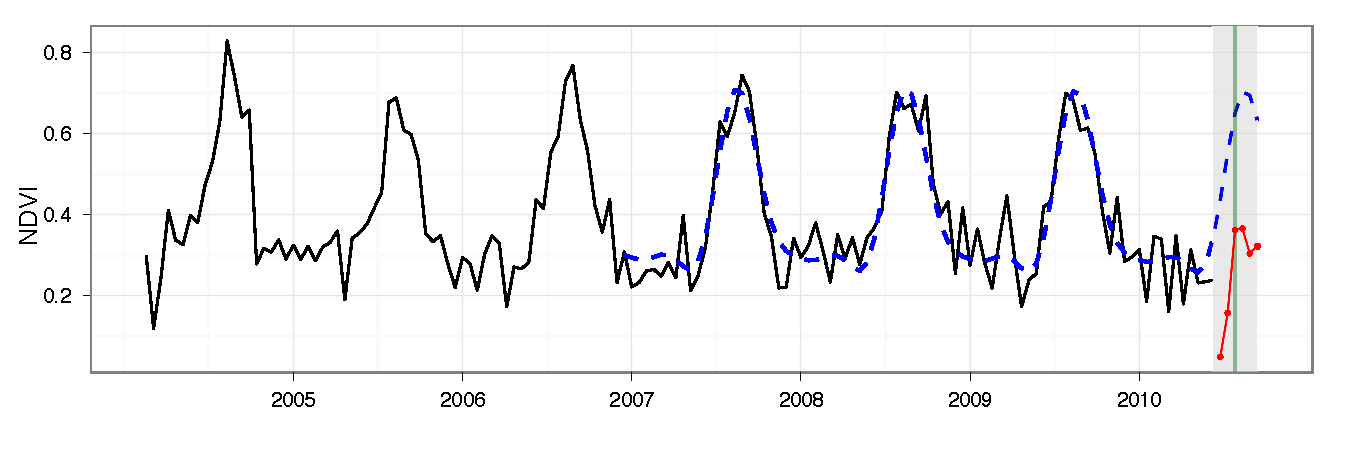
\includegraphics[width=1\textwidth]{figs/Sim_Monitoring_ggplot.pdf}
  \caption{Simulated 16-day MODIS NDVI time series with $a = 0.4$, $\sigma = 0.05$, containing one simulated abrupt change with $m = -0.3$). The period from
  2004 until mid 2010 (i.e., the time step just before the simulated break), is considered the \emph{history period} and the period after the simulated
  break is the \emph{monitoring period} (grey background). The monitoring period contains 6 observations  ($d = 6$, \textcolor{red} {red} line). The
  result of the monitoring approach are shown. A stable history period is identified within the history period (i.e.\ 2007 until mid 2010) and used to model
  and predict the normal data variation (\textcolor{blue} {blue} dashed line) to enable disturbance detection (Section~\ref{sec:MonStrucChange}).  Here, a
  disturbance is detected (\textcolor{OliveGreen} {green} vertical line).}
  \label{fig:SimMonitor}
\end{figure}

 \begin{figure}[htp]
\centering
    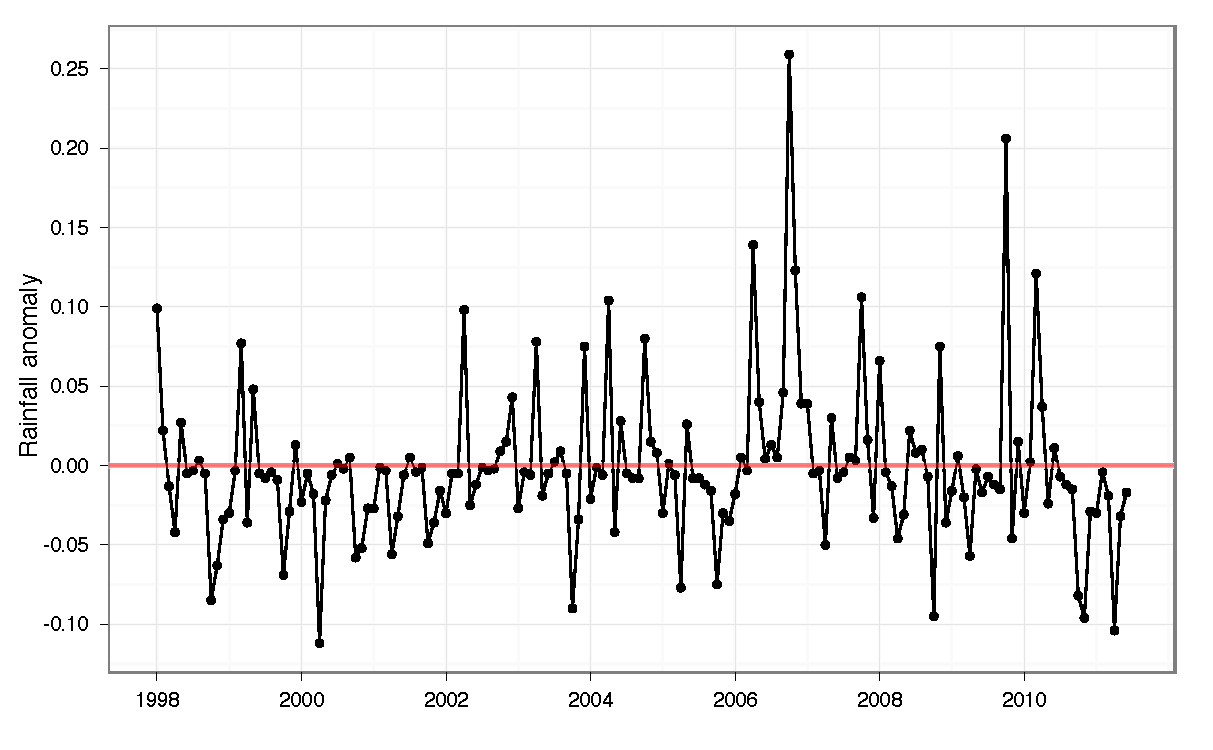
\includegraphics[width=0.8\textwidth]{figs/RainfallAnomaly.pdf}
  \caption{Monthly rainfall anomaly (mm/hr) for the period 1998--2011 measured by the tropical rainfall measuring satellite mission (TRMM) for an area in South Somalia (2\degree~Lat. and 43\degree~Long.). The time series was derived from the TRMM 3B43 climatology (version 6) data set using the online visualisation and analysis system (TOVAS). Anomalies are computed as the difference between the measured precipitation and the average climatology for the selected region \citep{Acker:2007vk}.}
  \label{fig:RF}
\end{figure}

\begin{figure} [htp]
\centering
 \subfloat[][] {\label{fig:RFA} 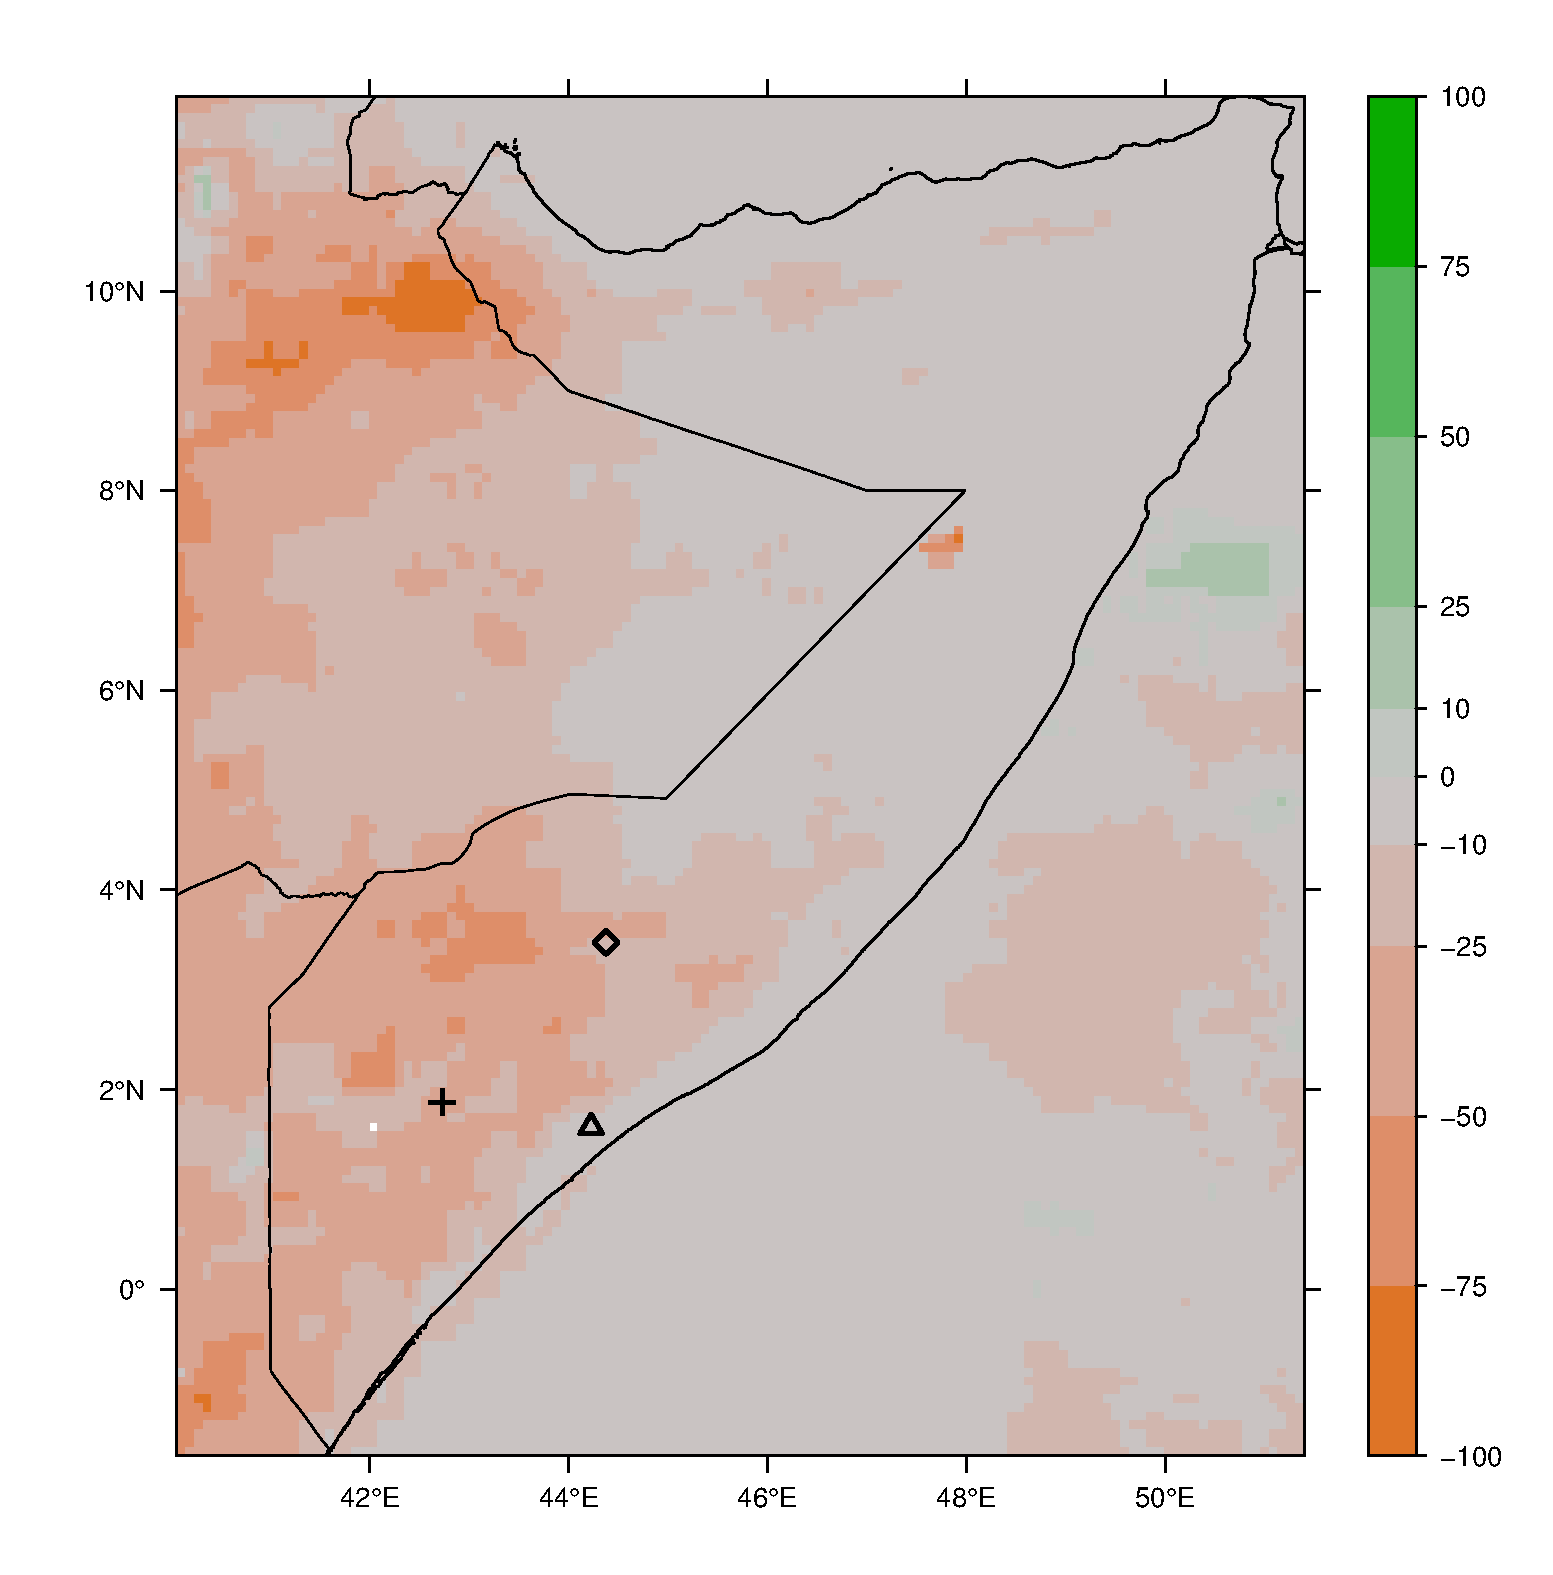
\includegraphics[height=0.55\textwidth]{figs/Rainfall_Somalia.png} } %
 \subfloat[][] {\label{fig:LST} 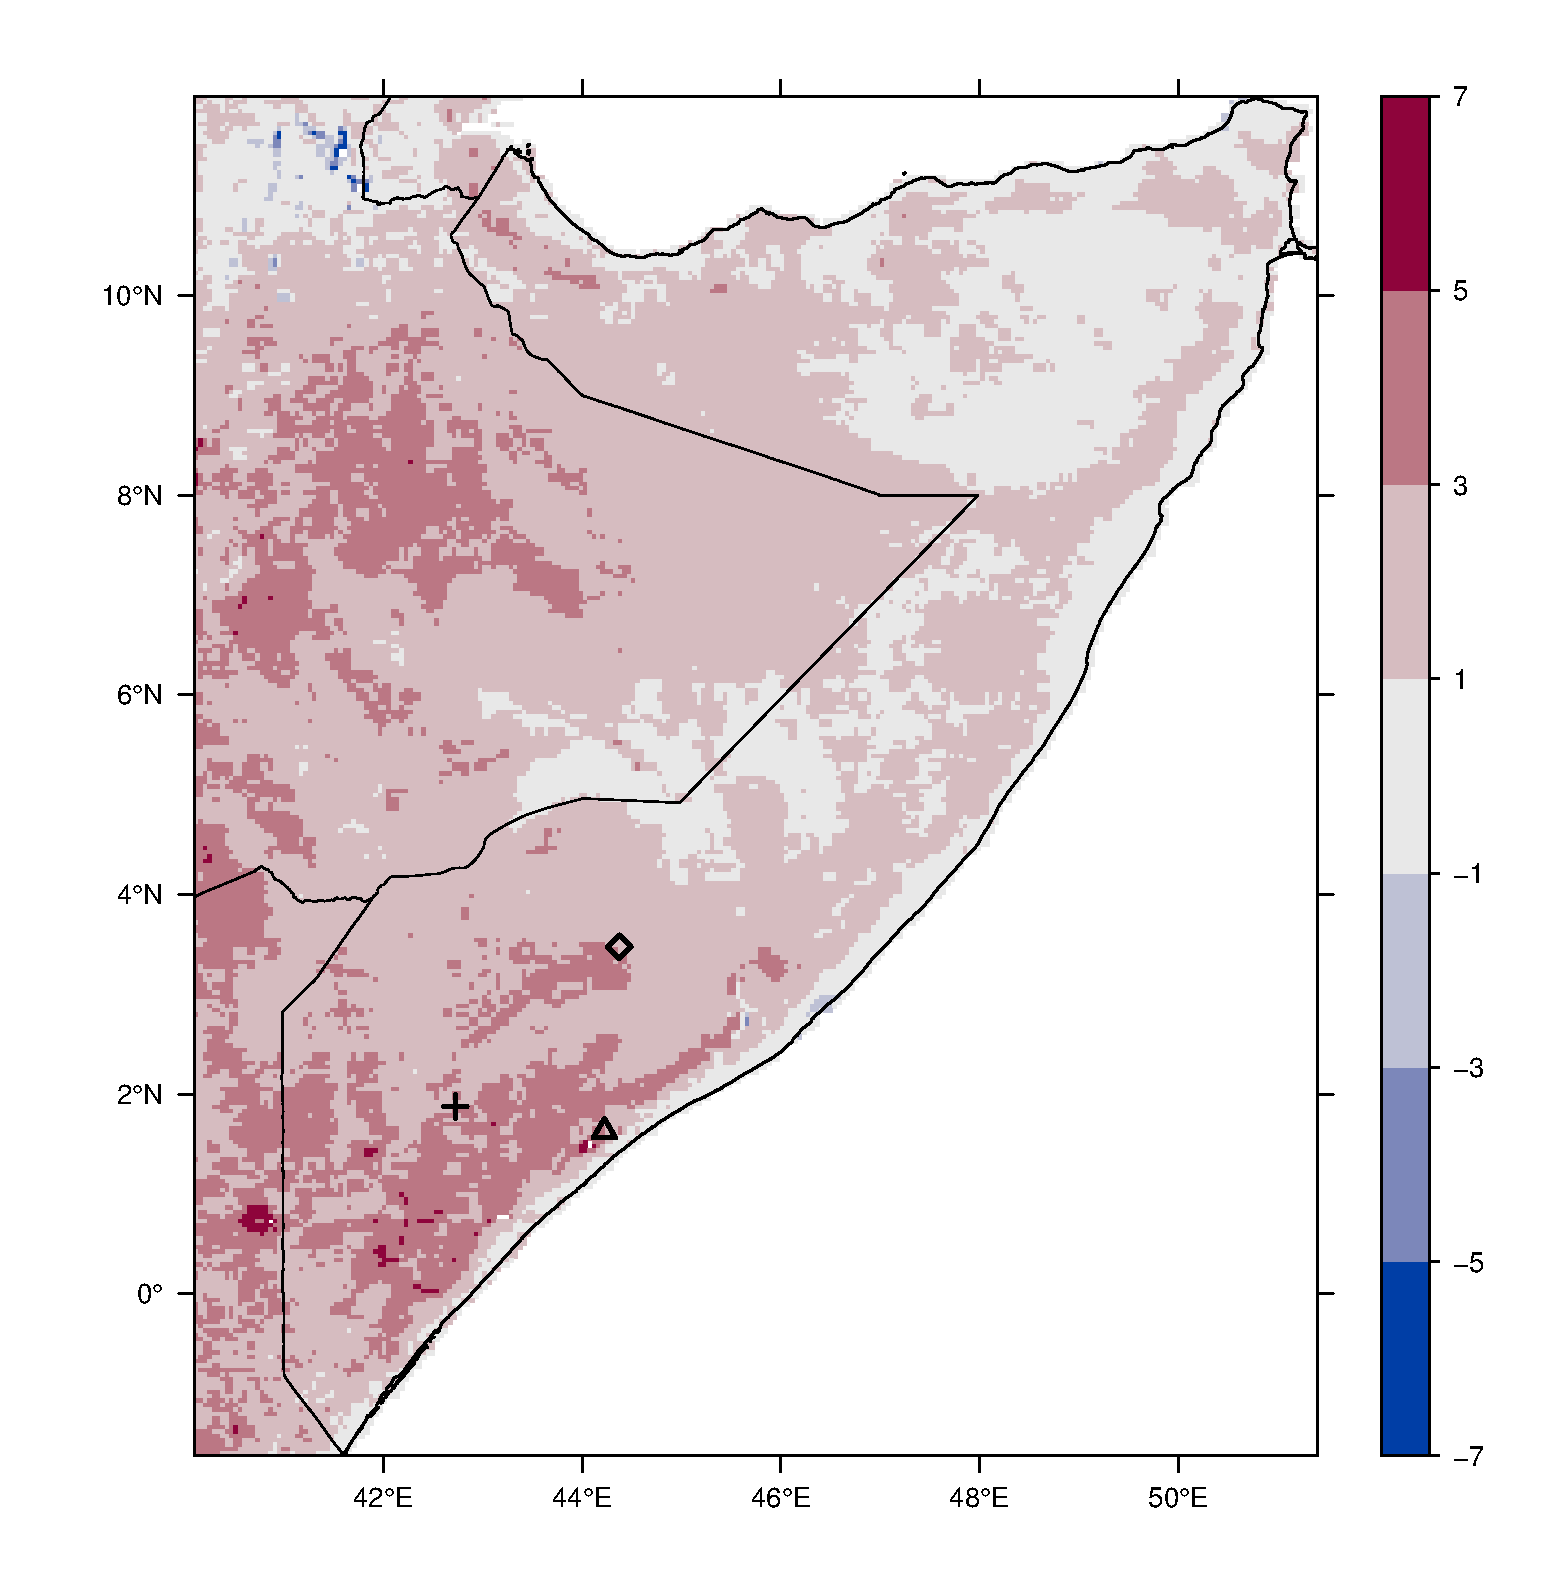
\includegraphics[width=0.55\textwidth]{figs/LSTMarchApril_Somalia.png} } 
 \caption{Two-monthly rainfall estimates (RFE2) (a)~and land surface temperature (LST) (b)~anomaly are shown for Somalia illustrating the below normal
 rainfall and above normal land surface temperature during the February-March period in 2011. The RFE2 data is a merged satellite-gauge rainfall product
 produced by NOAA's Climate Prediction Centre at a 0.1\degree spatial resolution. The LST product is the land surface temperature measured by the MODIS
 satellite and is provided at a 0.05\degree spatial resolution. Individual observations are subtracted from the time series mean to produce anomaly data. MODIS
 NDVI time series (2000--2011) for three locations ($\triangle,+$~and~$\diamondsuit$) are shown in Fig.~\ref{fig:realmon}. The data was obtained using the Early Warning Explorer software tool available at \url{earlywarning.usgs.gov}. }
 \label{fig:RF_LSTSomalia}
\end{figure}

\begin{figure}[htp]
\centering
    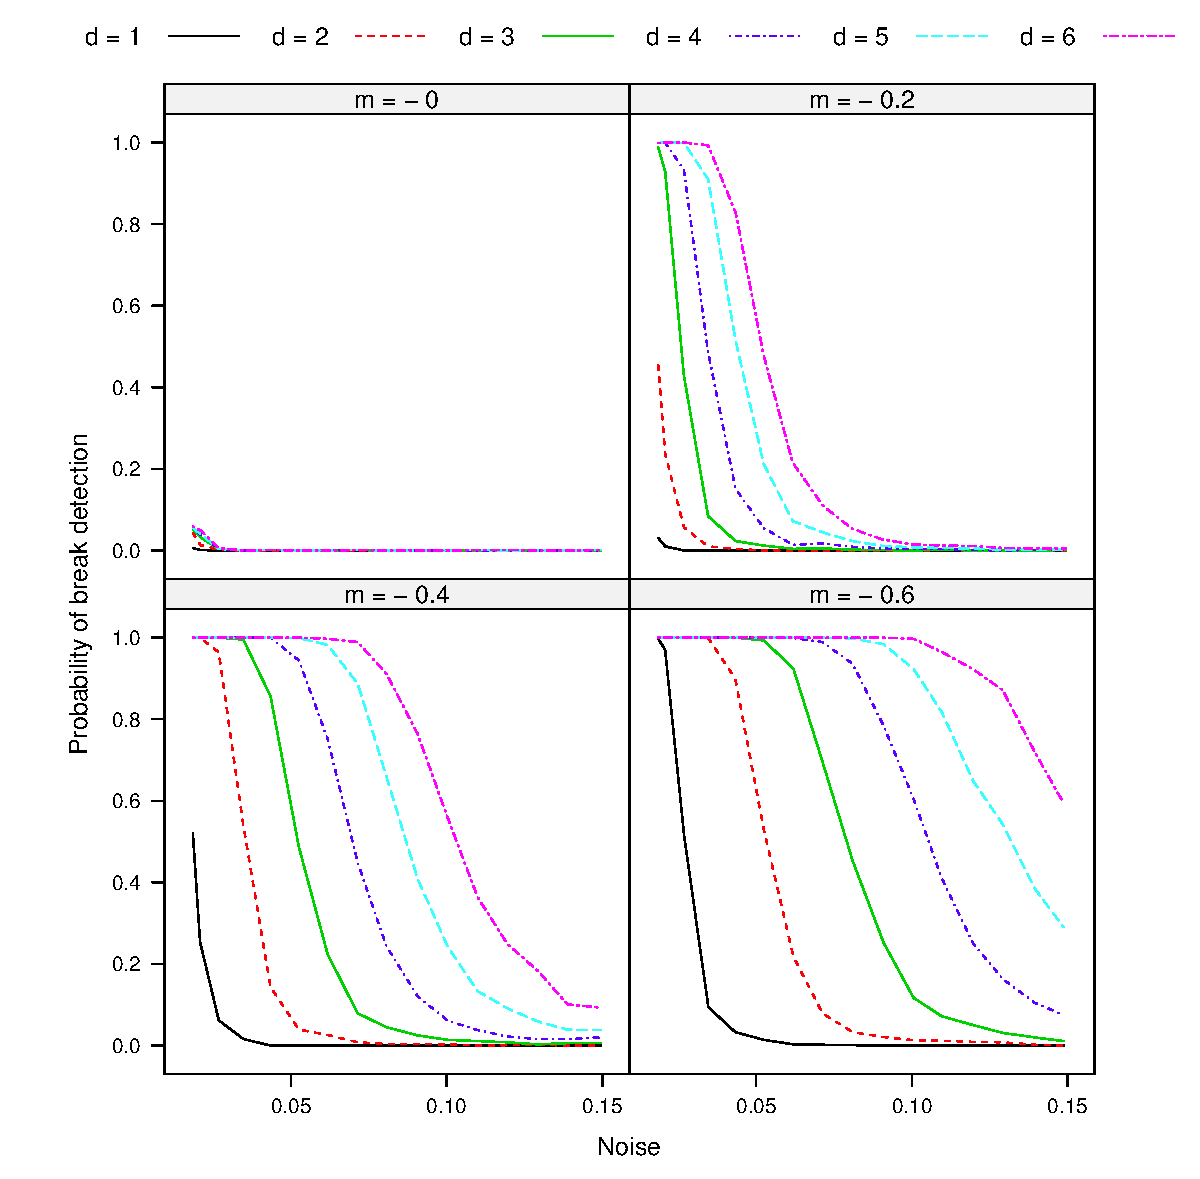
\includegraphics[height=0.9\textwidth]{figs/NrDetections_Time_1000.pdf}
  \caption{Results from the simulation experiment (1000 iterations) illustrating the probability for break detection in the monitoring period while varying the amount of noise ($\sigma$), magnitude of the simulated break ($m$), and amount of data  available in the monitoring period ($d$). The units of the x and y-axis are noise (i.e., $\sigma$ NDVI of the residuals of the fitted season-trend model on the history period) and probability of detecting a break (i.e., proportion of detected breaks in 1000 iterations). See description of the simulation experiment for more details (Section~\ref{sec:Valsim}). }
  \label{fig:SimNr}
\end{figure}

\begin{figure}
\centering
 \subfloat[][] {\label{fig:spatiala} 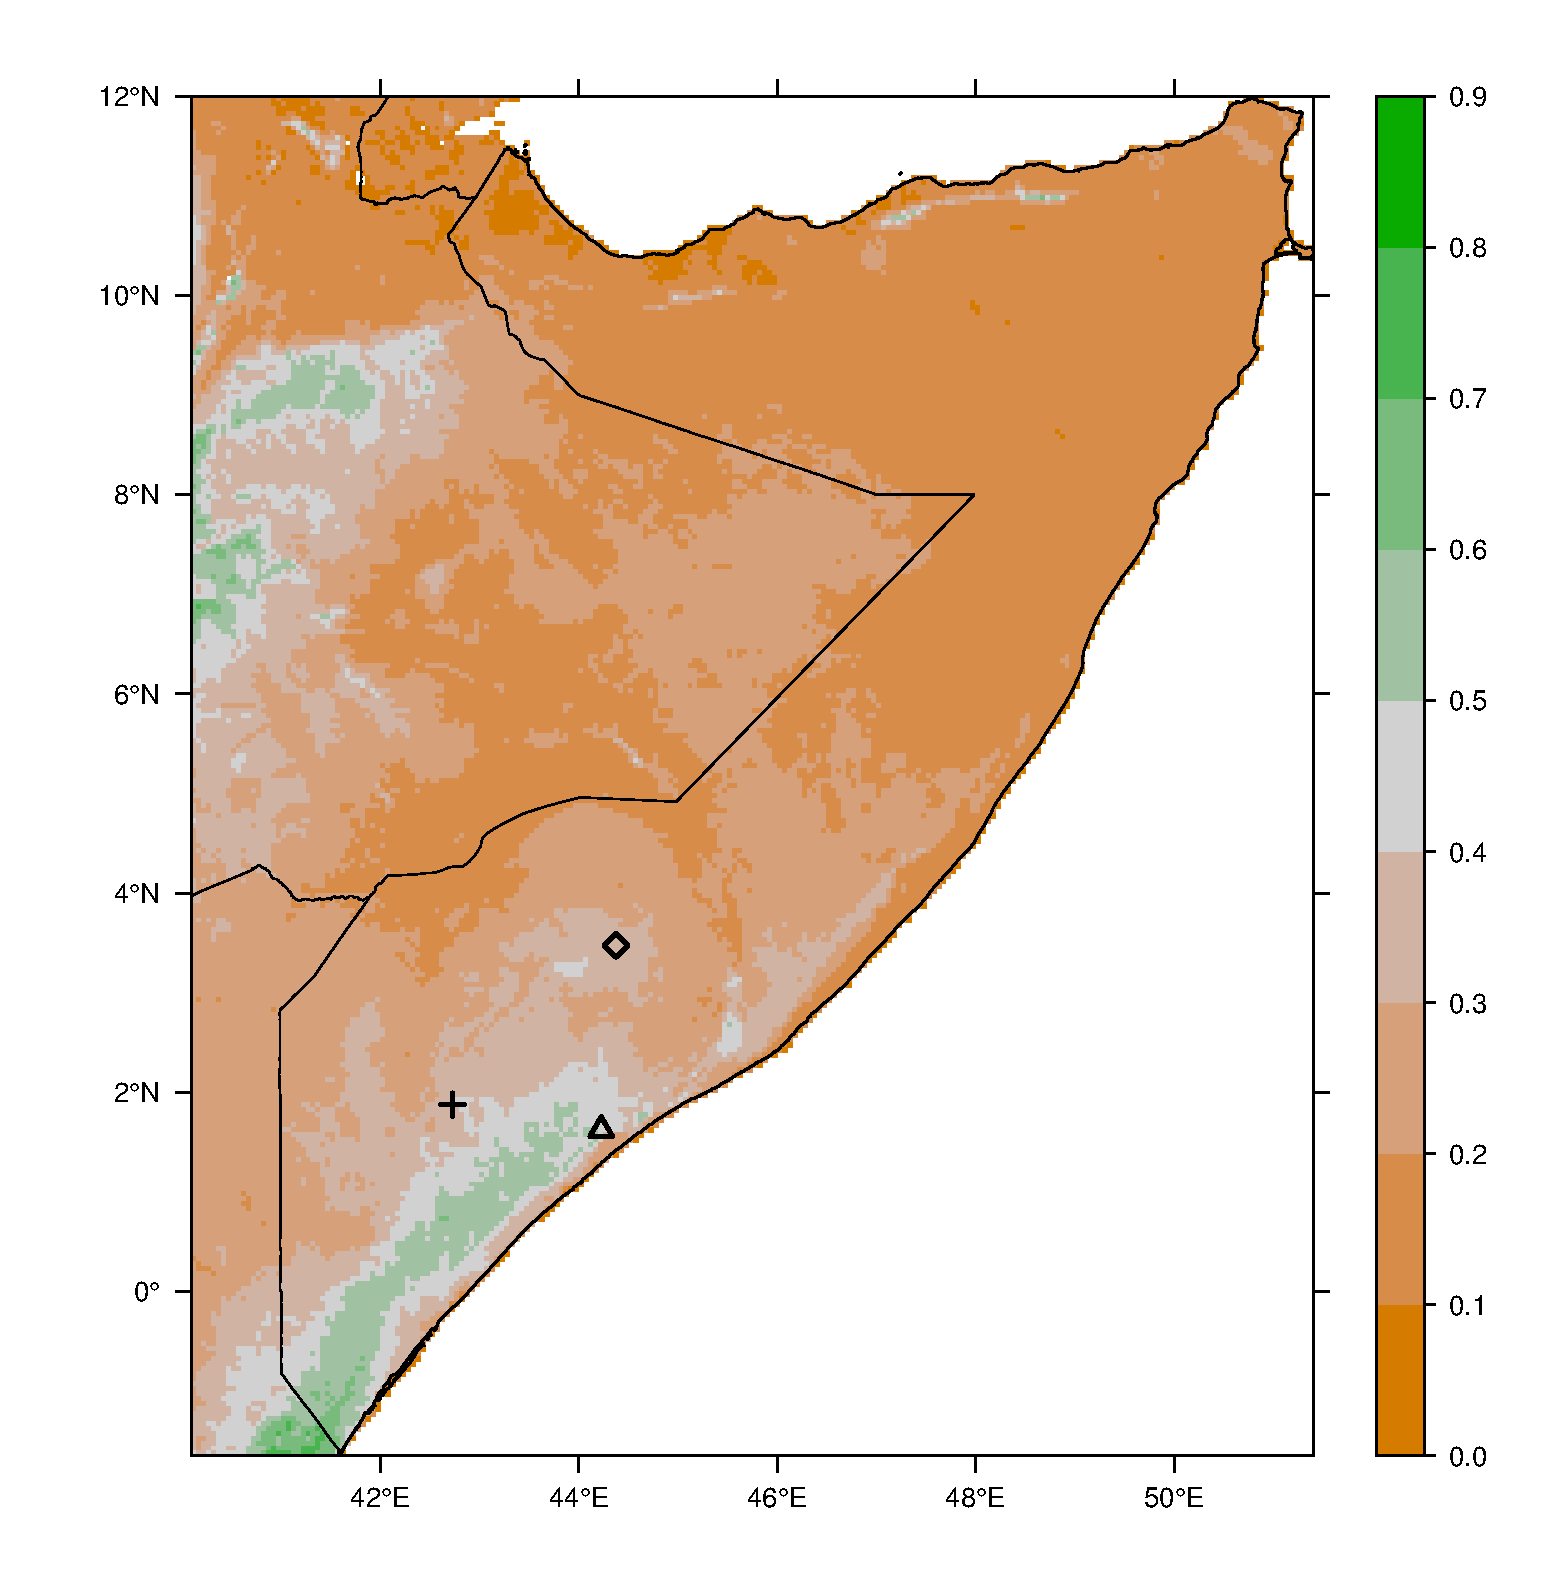
\includegraphics[height=0.55\textwidth]{figs/MedianNDVI_Somalia.png} } %
 \subfloat[][] {\label{fig:spatialb} 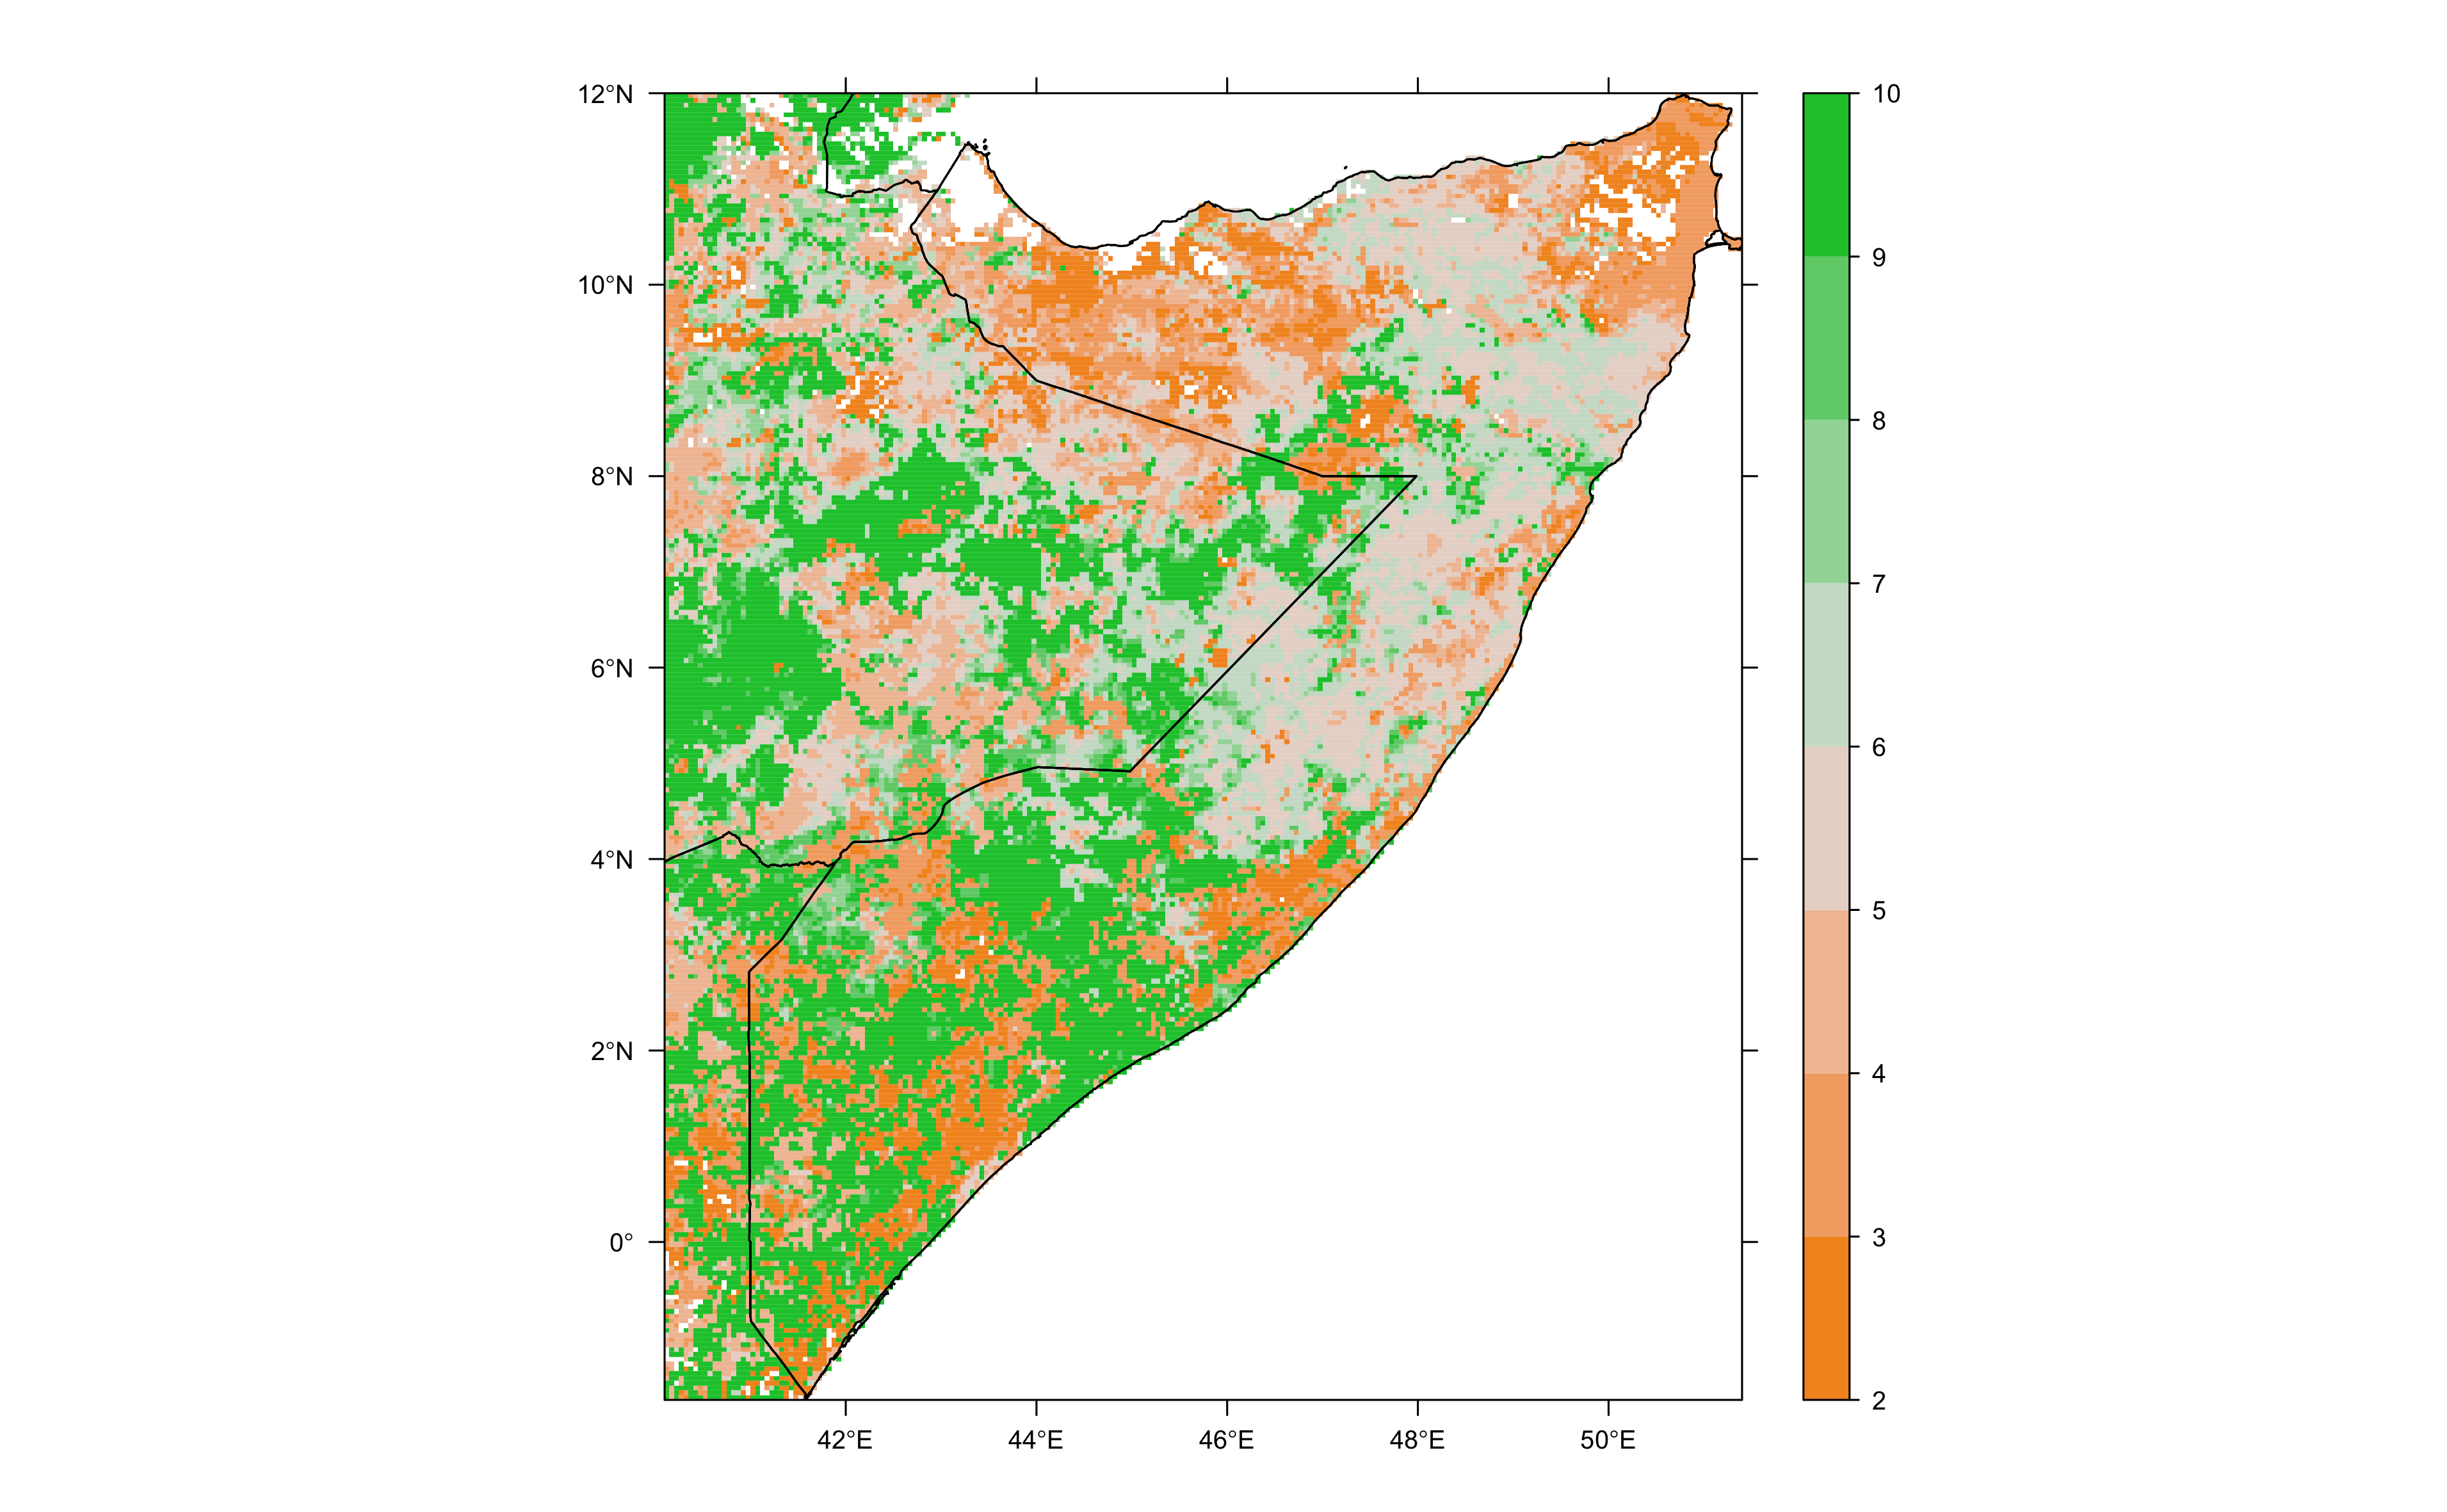
\includegraphics[width=0.55\textwidth]{figs/LengthHistoryPeriod_EA.png} }  \\
 \subfloat[][] {\label{fig:spatialc} 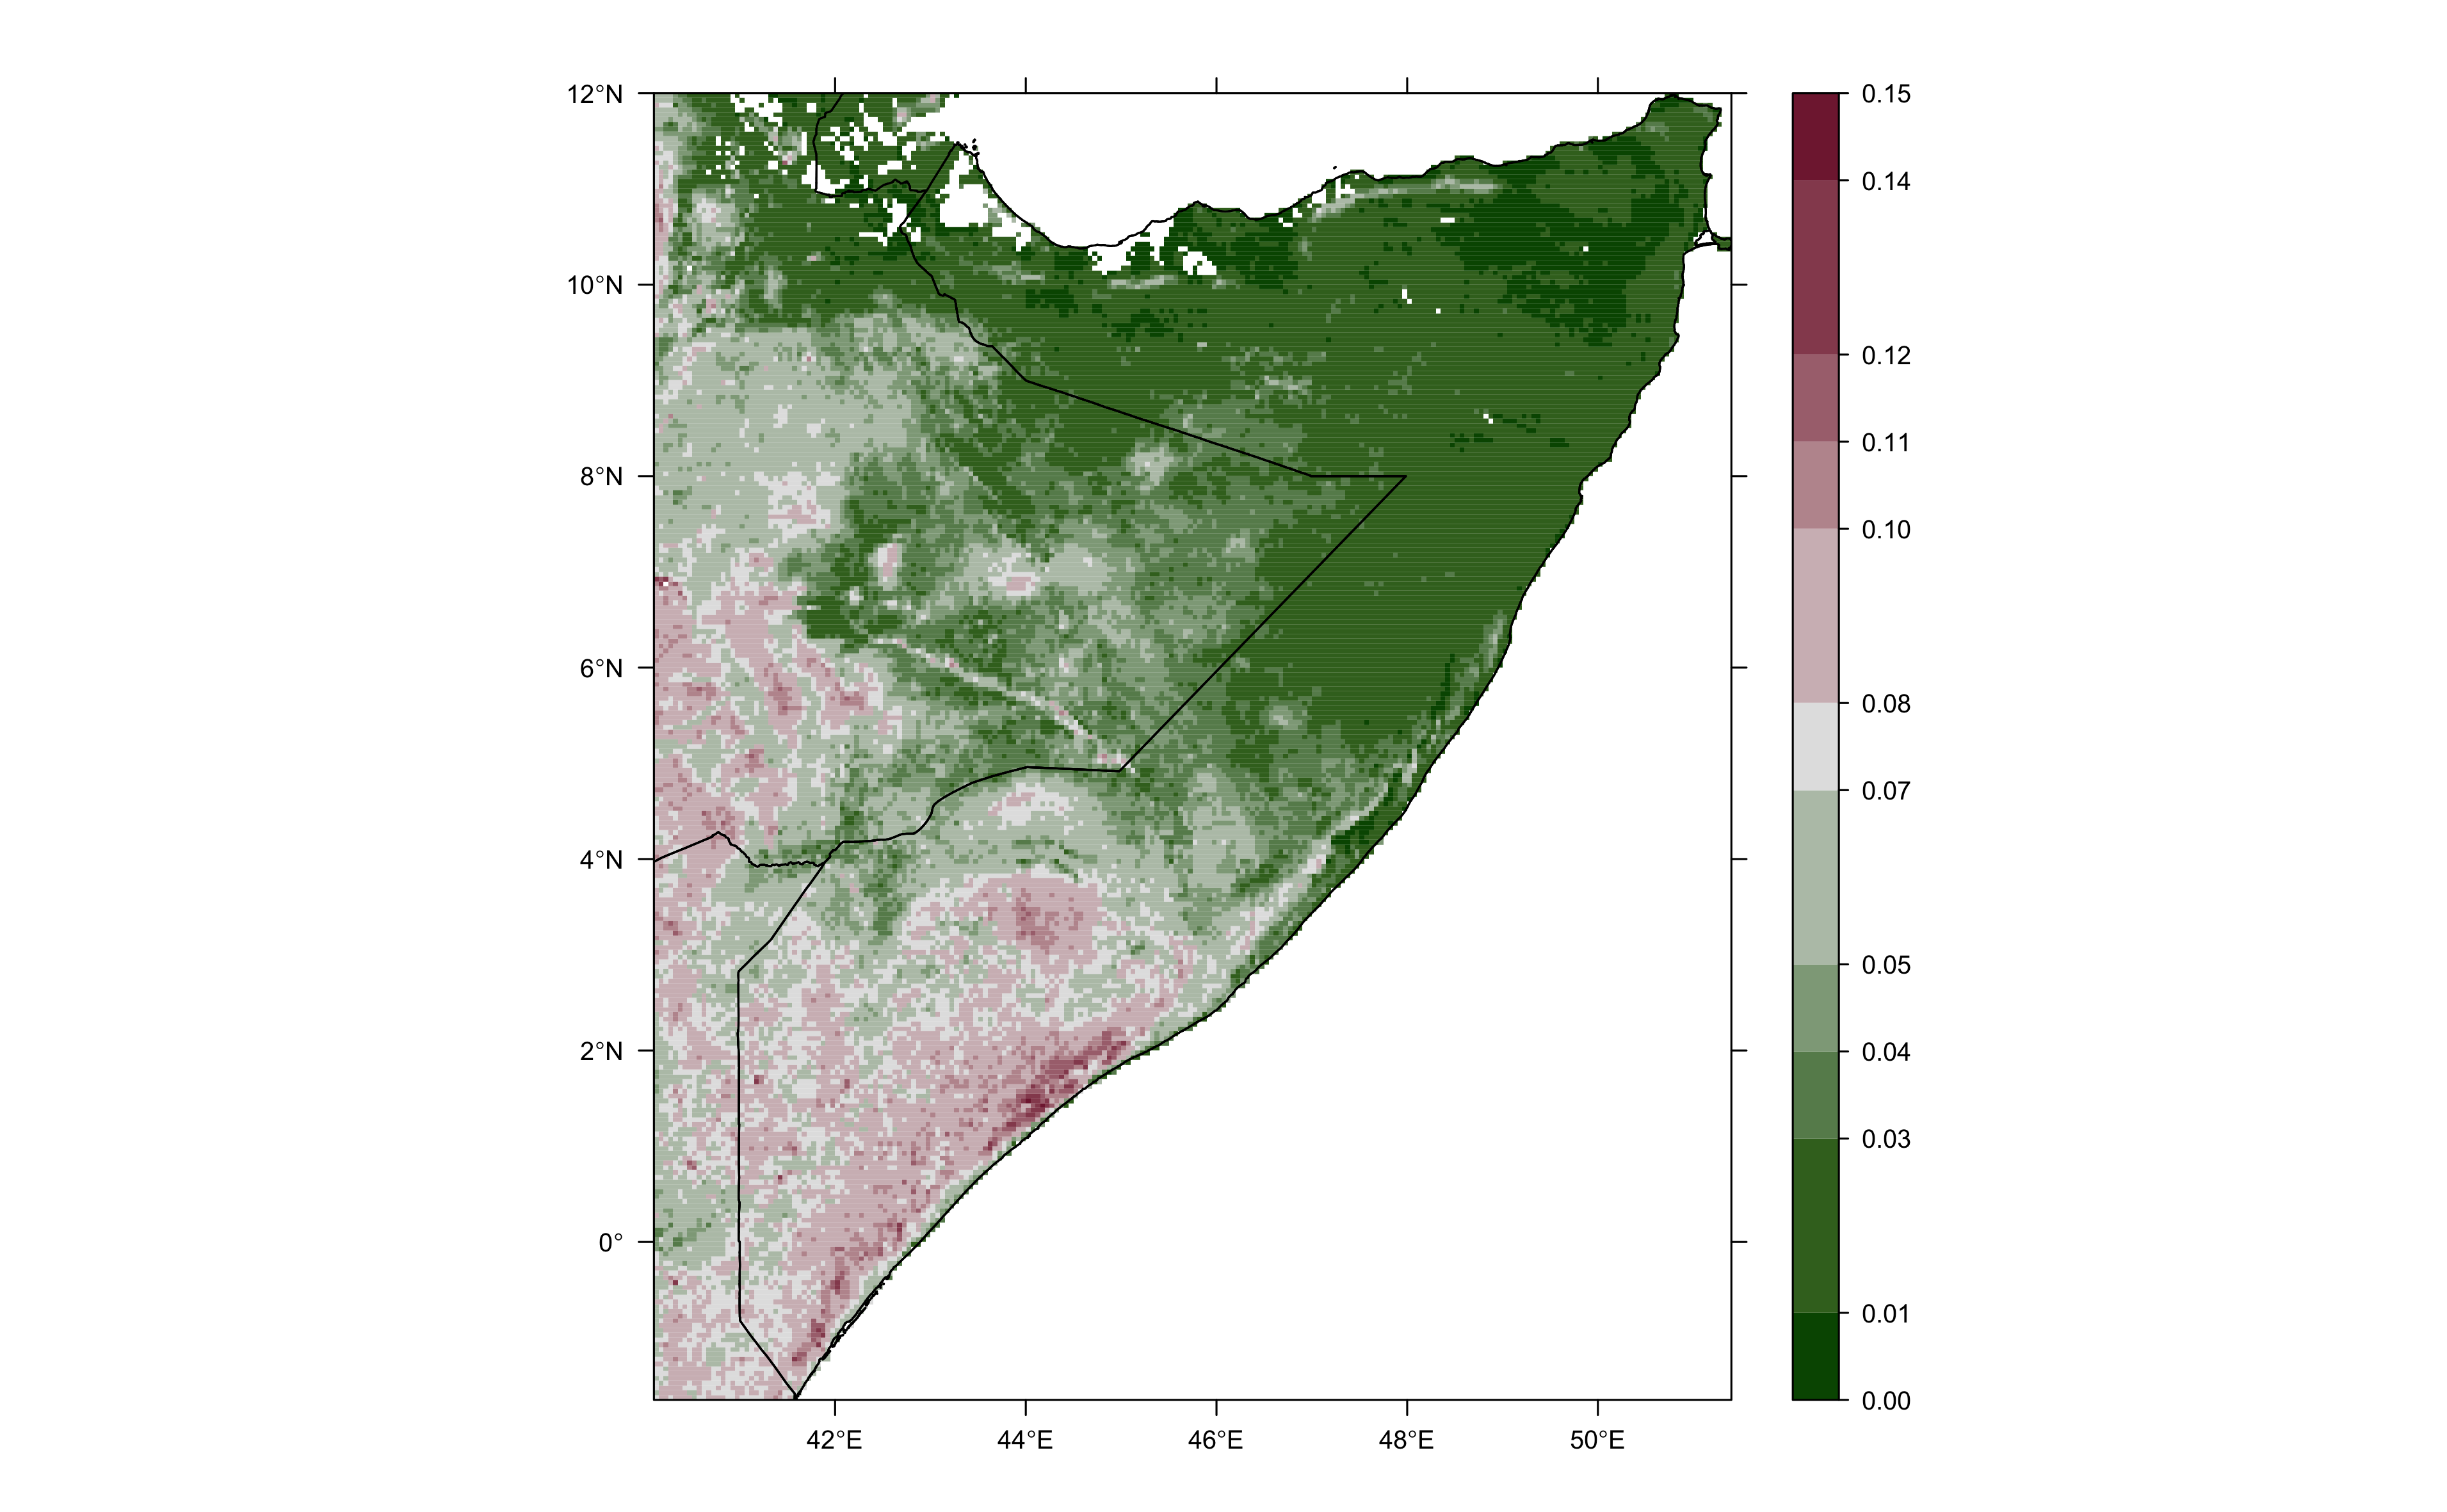
\includegraphics[width=0.55\textwidth]{figs/Noise_EA.png} } %
\subfloat[][] {\label{fig:spatiald} 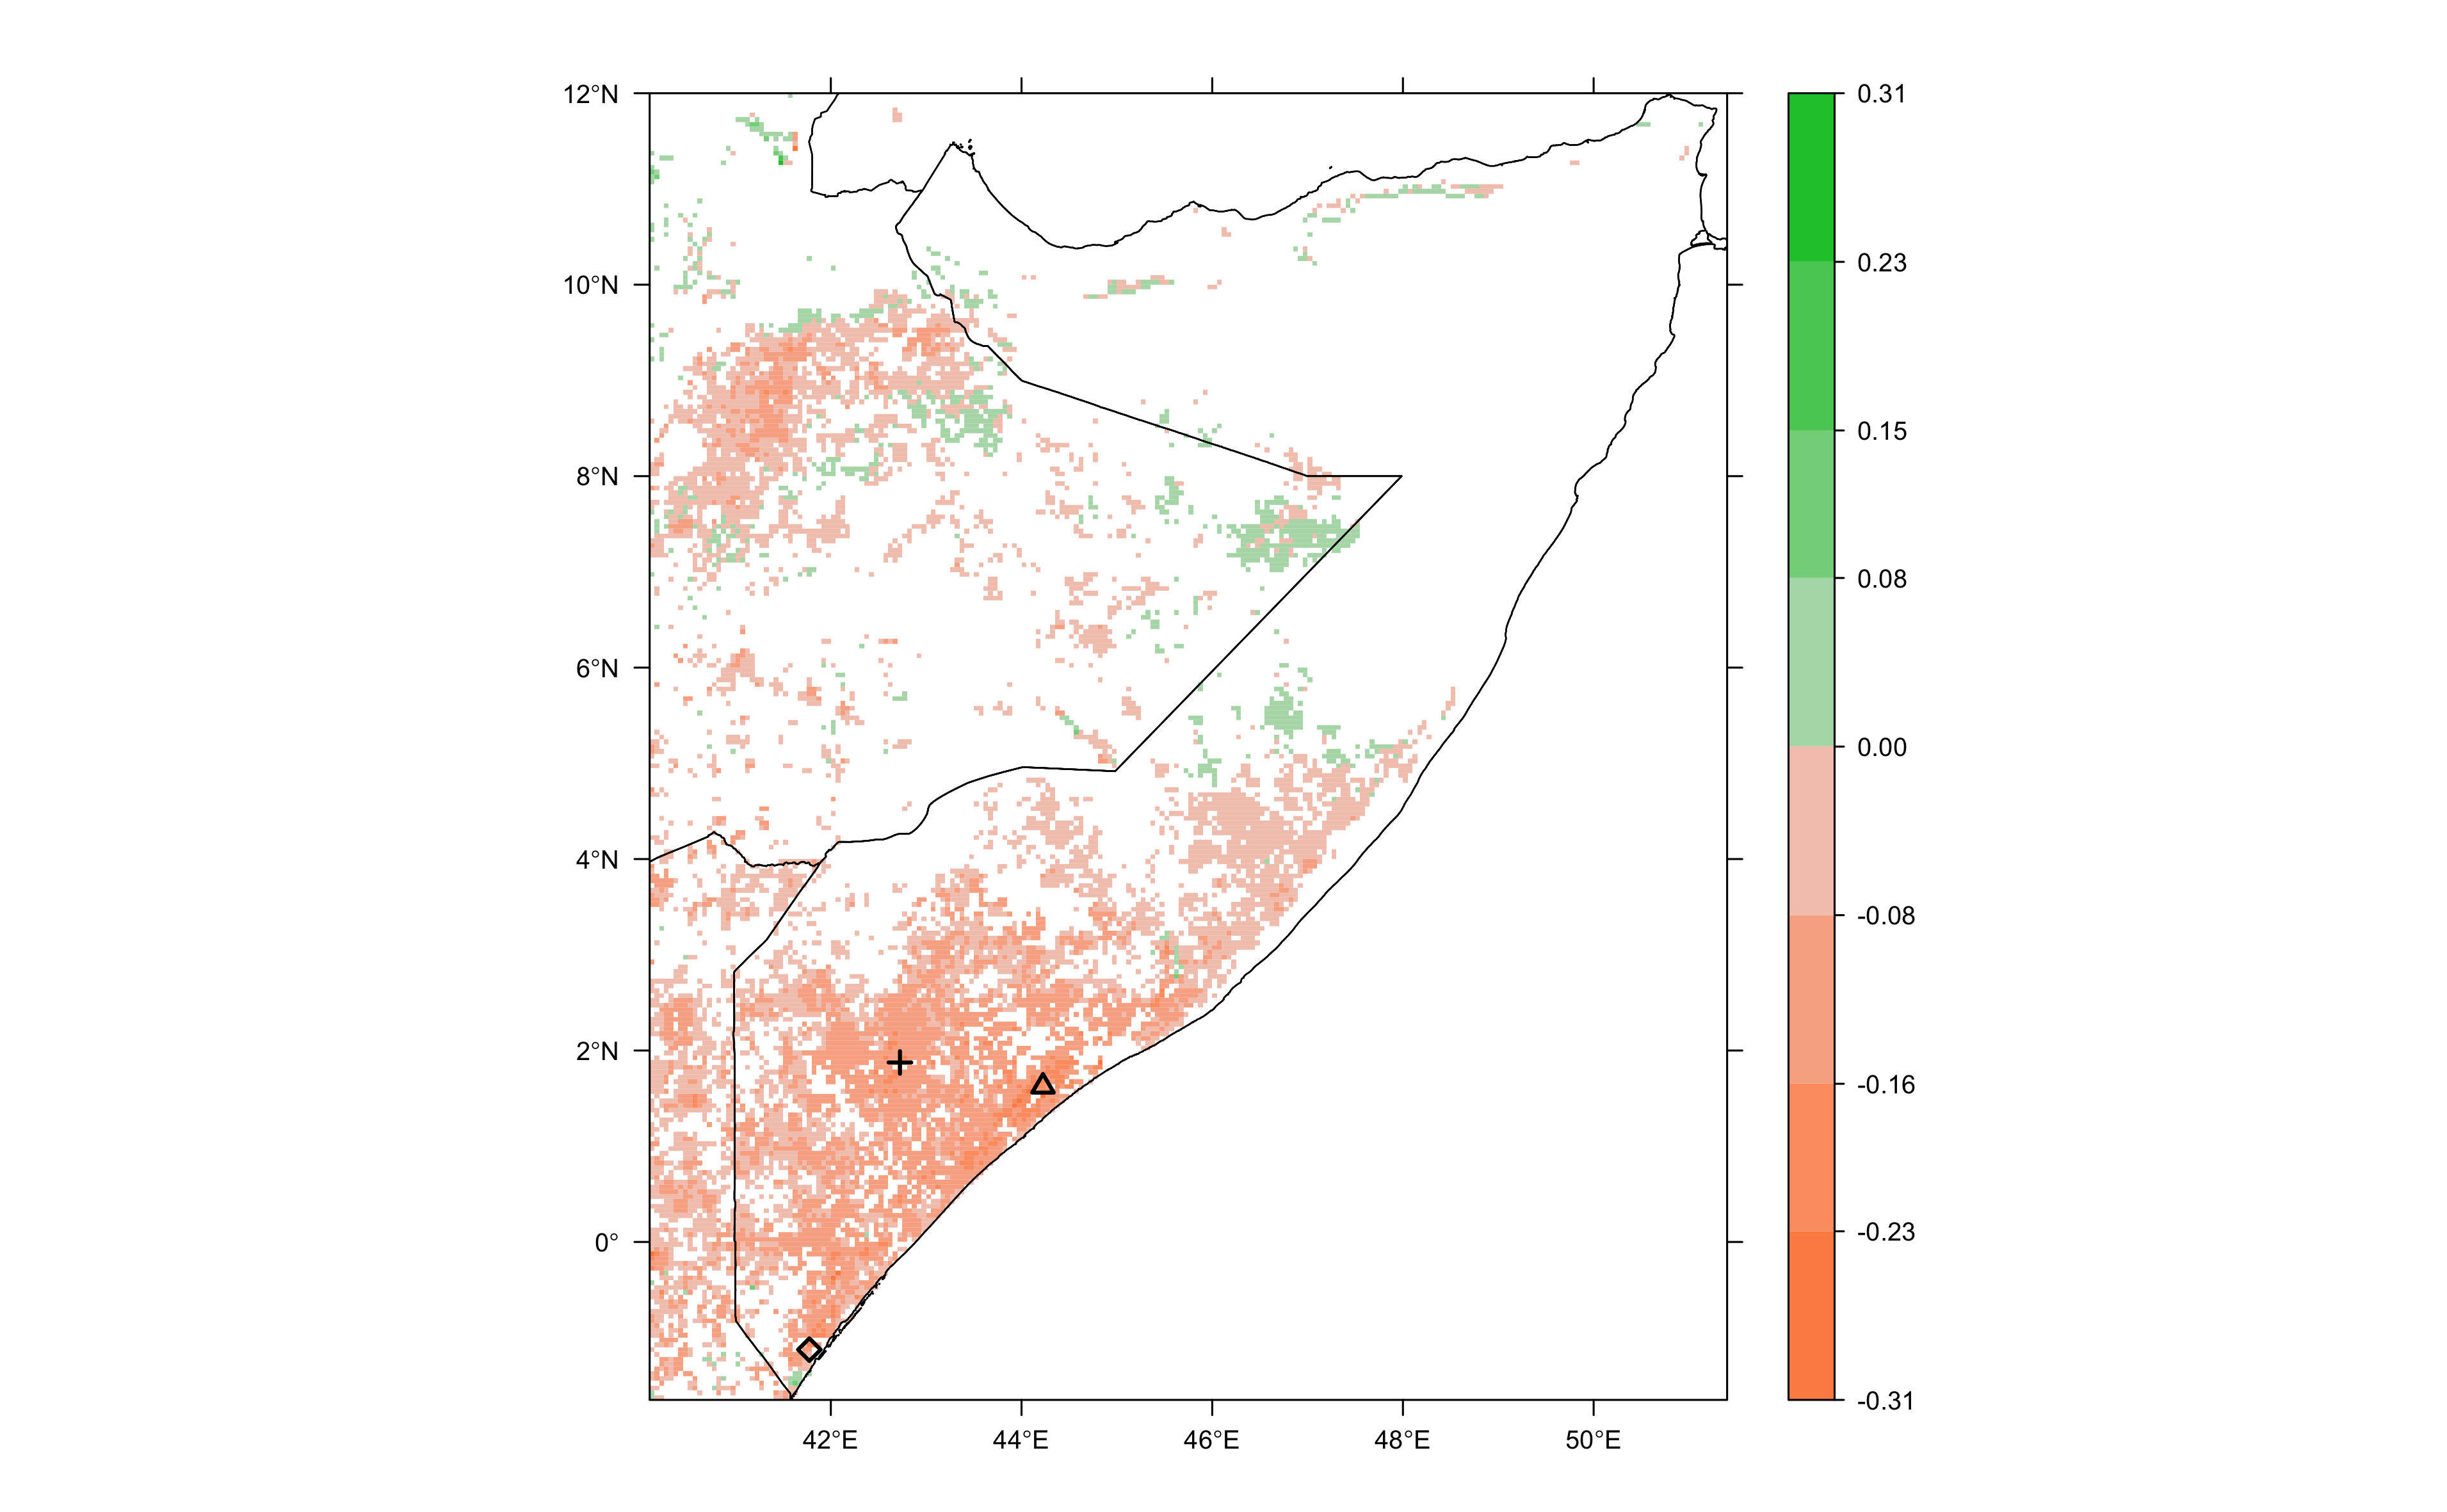
\includegraphics[width=0.55\textwidth]{figs/MagnAbnormalBreak_201012_EA.png} }
 \caption{Results from the analysis of 16-day MODIS NDVI image time series from February 2000 until July 2011 covering Somalia; (a)~median of all NDVI
 images as a proxy for vegetation cover during the 2000--2011 period, (b)~length of the stable history period expressed in years where a shorter length is
 an indication of a more recent disturbance, (c)~spatial variation of the noise level i.e.\ the standard deviation of the residuals of the stable history
 model, (d)~the magnitude of the detected disturbances in the monitoring period (mid 2010 onwards) where white indicates that no disturbance is detected. 
 The analysis of~(d)
 was restricted to areas with minimum vegetation cover i.e.\ median NDVI  2000--2011$> 0.2$ and length of the history period $> 2$ years. Examples for three locations ($\triangle,+$~and~$\diamondsuit$) are shown in Fig.~\ref{fig:realmon}.}
 \label{fig:spatial}
\end{figure}

\begin{figure}[htp]
\centering
    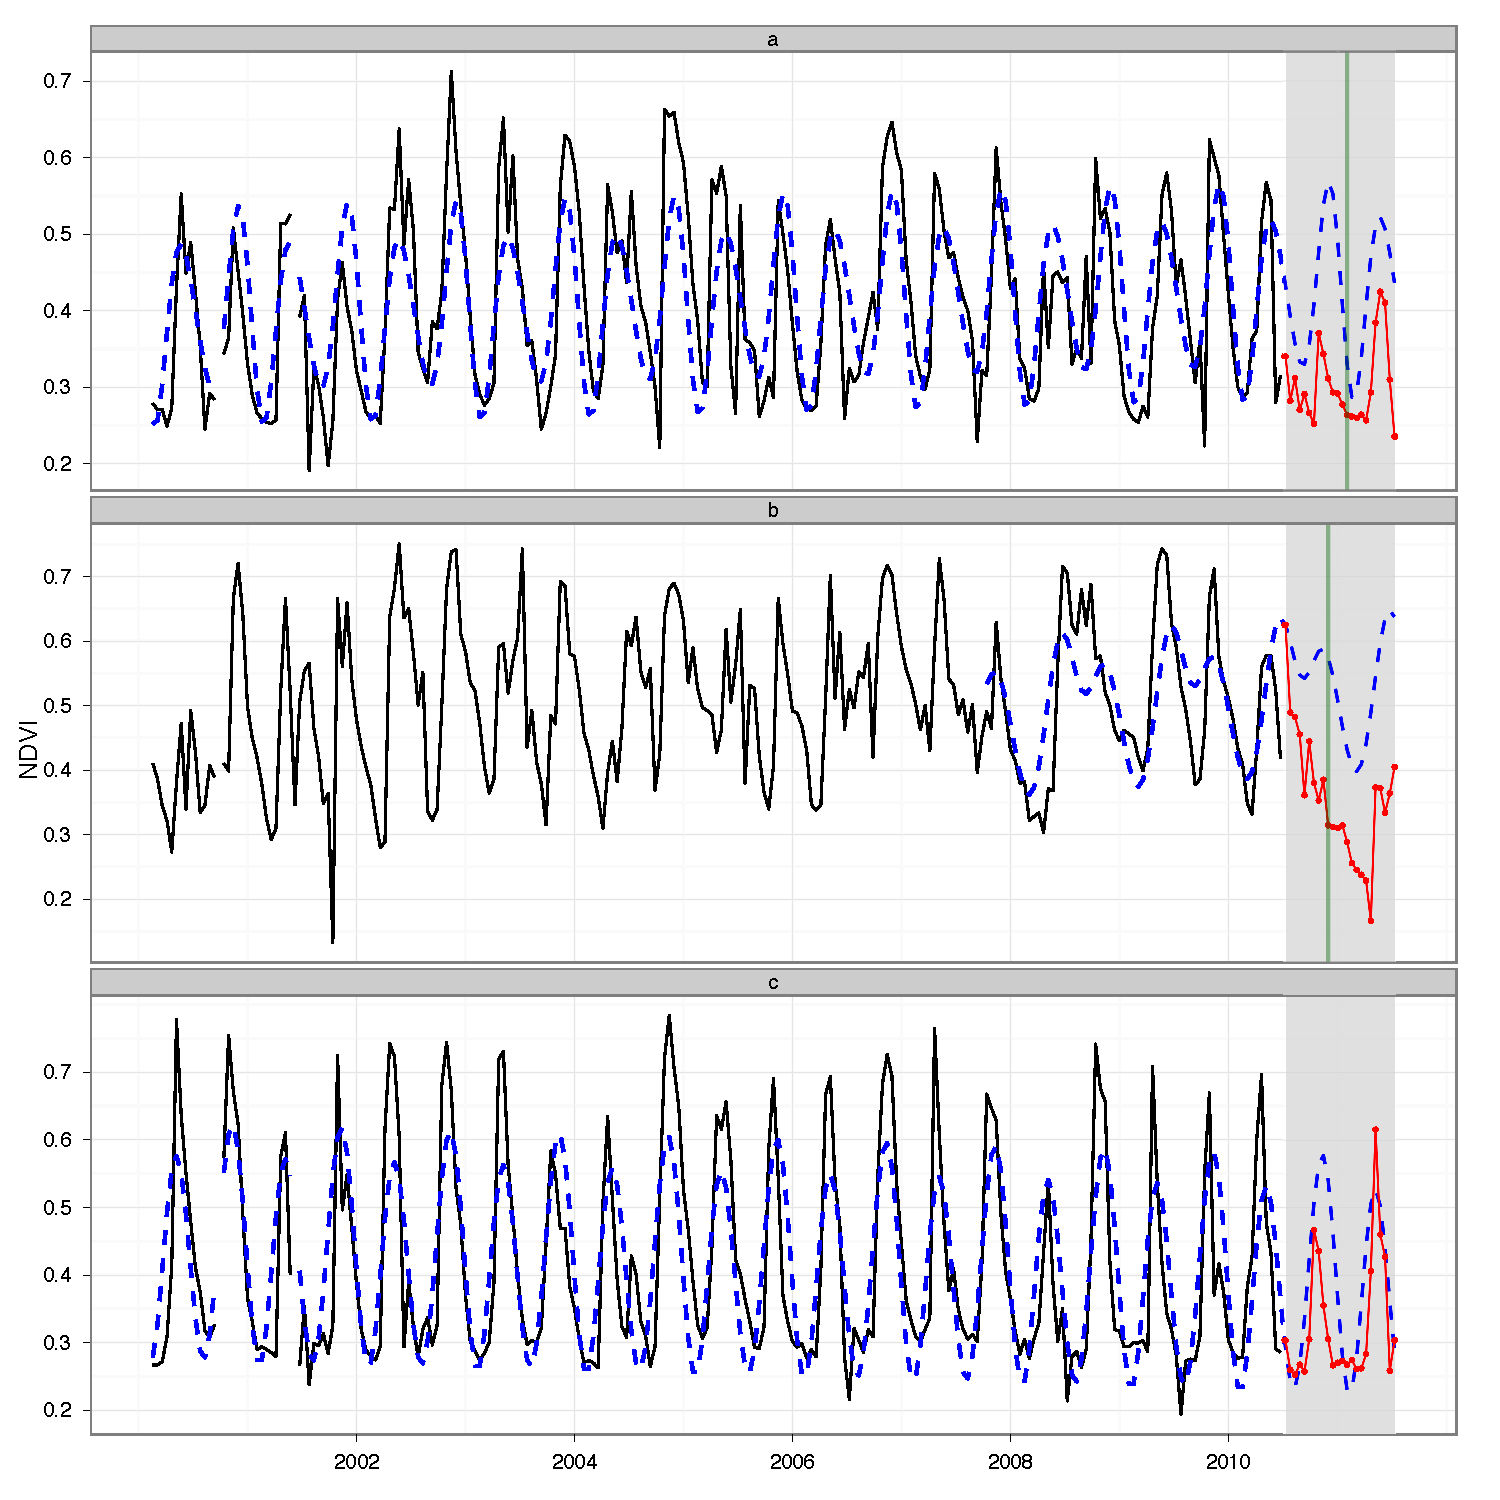
\includegraphics[width=1\textwidth]{figs/tsexampleSOM.pdf}
  \caption{
 Results of real-time monitoring approach applied to 16-day MODIS NDVI time series for three locations a, b, and c, corresponding to symbols
 $+,~\triangle$~and~$\diamondsuit$ shown in Fig.~\ref{fig:spatial}. The period from 2000 until mid 2010, is considered the \emph{history period} and the
 period after the simulated break is the \emph{monitoring period} (grey background, \textcolor{red} {red} line). The stable history period within the
 history period (\textcolor{blue} {blue} dashed line) is used to model and predict the normal data variation and enable disturbance detection in the
 monitoring period (Section~\ref{sec:MonStrucChange}).  A disturbance is detected (\textcolor{OliveGreen} {green} line) in Fig~\ref{fig:spatiala} and~\ref{fig:spatialb}.}
 
% In both time series a break (vertical red dashed line in 2006) is detected in the monitoring period (i.e., 2006) while using 2000 until end of 2005 as a history period. A stable history period (blue dots) is automatically detected with the history period. The method is able to deal with time series with data gaps (e.g., after cloud removal) which is illustrated by data gaps within the data analysed and model fit based on the stable history period.

  \label{fig:realmon}
\end{figure}


%% explain the monitoring period
%% the model
%% break
%% etc.
%%, i.e., $\diamondsuit$ (top) and $\triangle$ (bottom) on Fig.~\ref{fig:SpatNoise},~\ref{fig:SpatTimeofChange} and~\ref{fig:SpatLStableHist}), situated within the Green Hills study area
%

%%\begin{figure}[htp]
%%\centering
%%    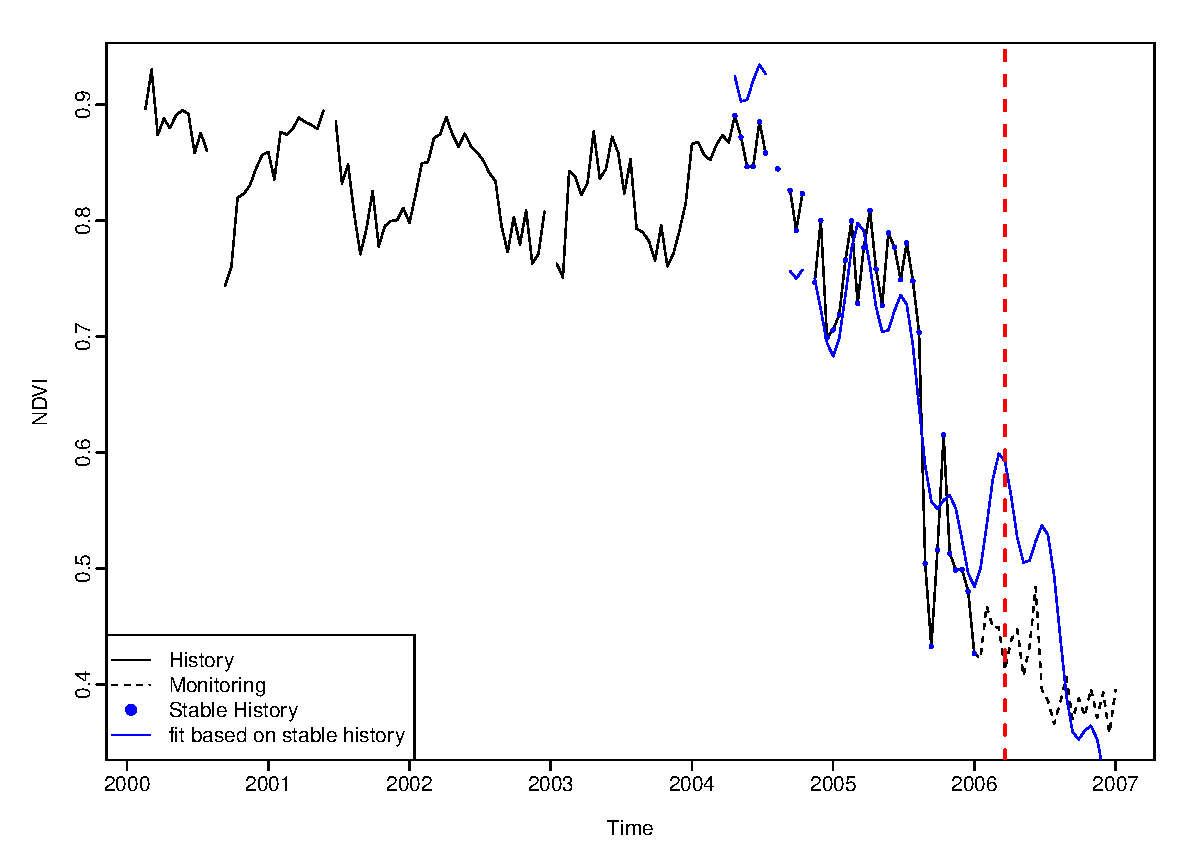
\includegraphics[height=0.6\textwidth]{figs/shorthistoryperiod.eps}
%%  \caption{
%%  Results of real-time monitoring approach applied to 16-day MODIS NDVI time series for a location situated within the Green Hills study area (i.e., the $+$ symbol on Fig.~\ref{fig:SpatNoise}, \ref{fig:SpatTimeofChange} and~\ref{fig:SpatLStableHist}). A break (vertical red dashed line in 2006) is detected in the monitoring period (i.e., 2006) while using 2000 until end of 2005 as a history period. A short stable history period (blue dots) is detected within the history period due to an ongoing harvest operation from 2005 onwards. The method is able to deal with time series with data gaps (e.g., after cloud removal) which is illustrated by data gaps within the data analysed and model fit based on the stable history period.}
%%  \label{fig:shorthistory}
%%\end{figure}

\end{document}

% %Examples of real-time change analysis for three locations ($\triangle,+$~and~$\diamondsuit$) are shown in Fig.~\ref{fig:realmonitoring} and~\ref{fig:shorthistory}. 
%\begin{figure}[htp]
%\centering
%    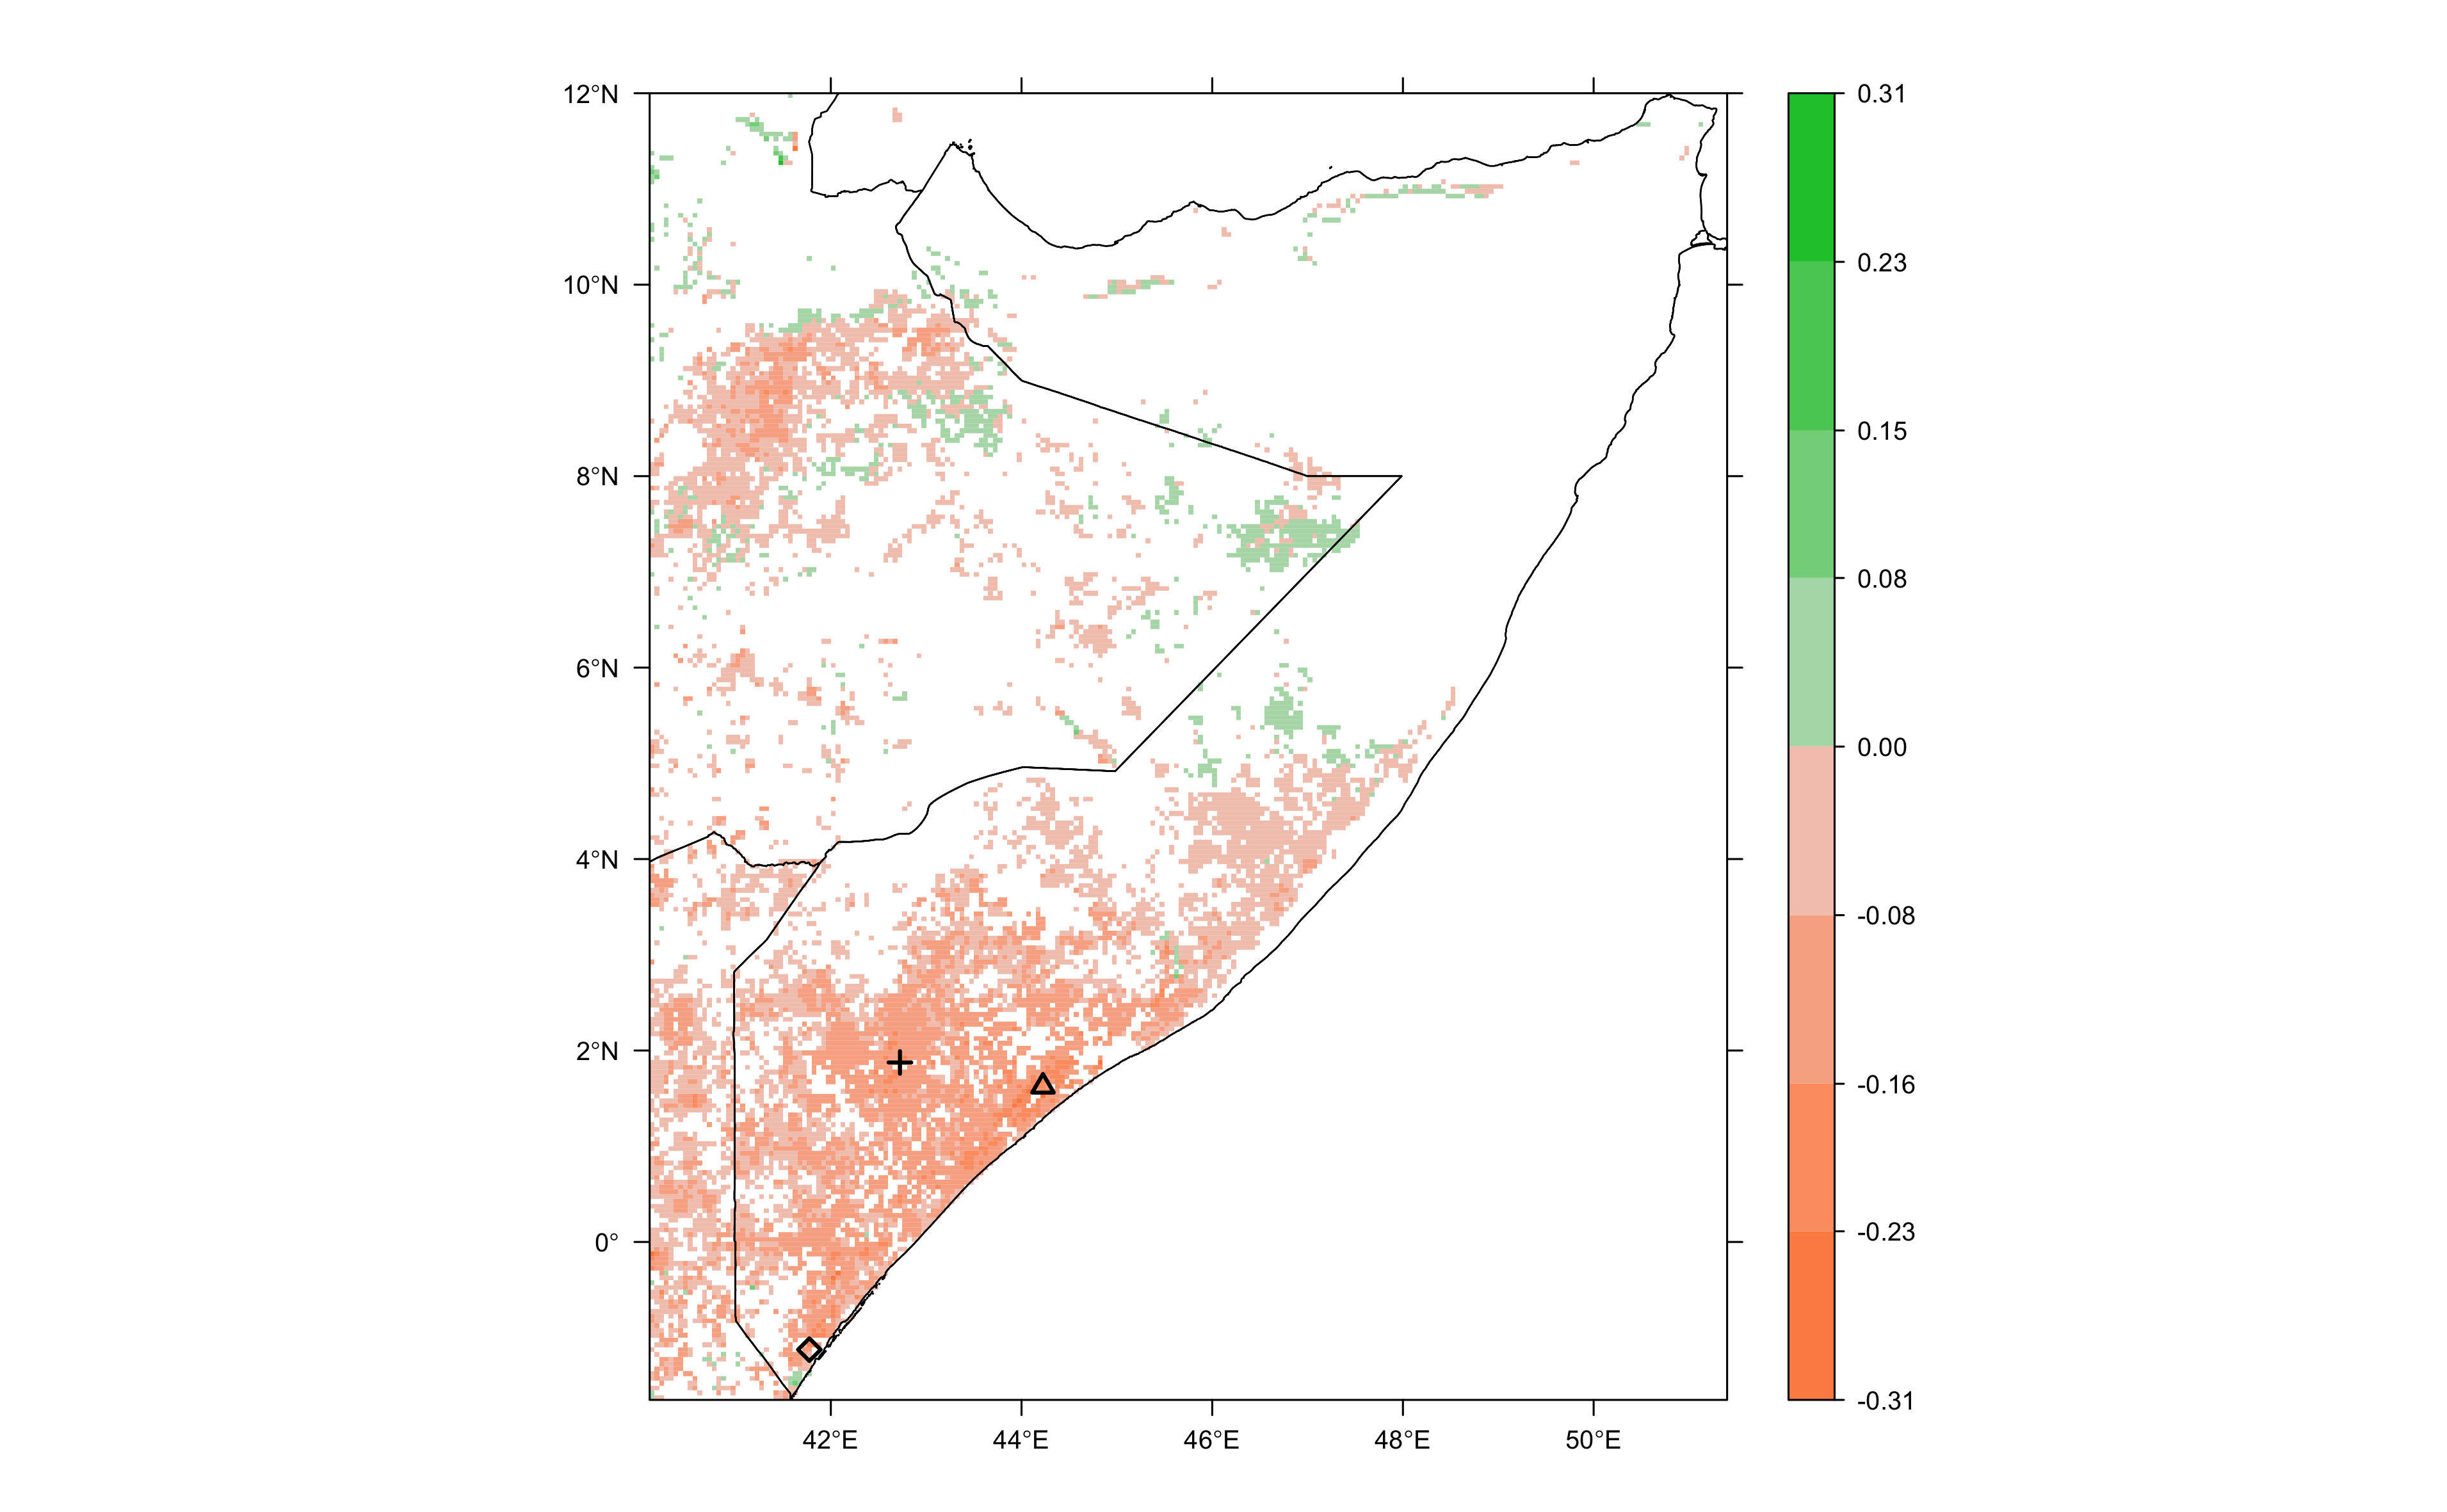
\includegraphics[height=0.7\textwidth]{figs/MagnAbnormalBreak_201012_EA.png}
%  \caption{Time of detected changes within the Eastern Africa during the monitoring period (2010--2011), where white indicates that no change is detected.  }
%  \label{fig:SpatTimeofChange}
%\end{figure}

%% I included png format figures - to reduce the filesize - but will submit .eps figures to global change biology!
%\begin{figure}[htp]
%\centering
%    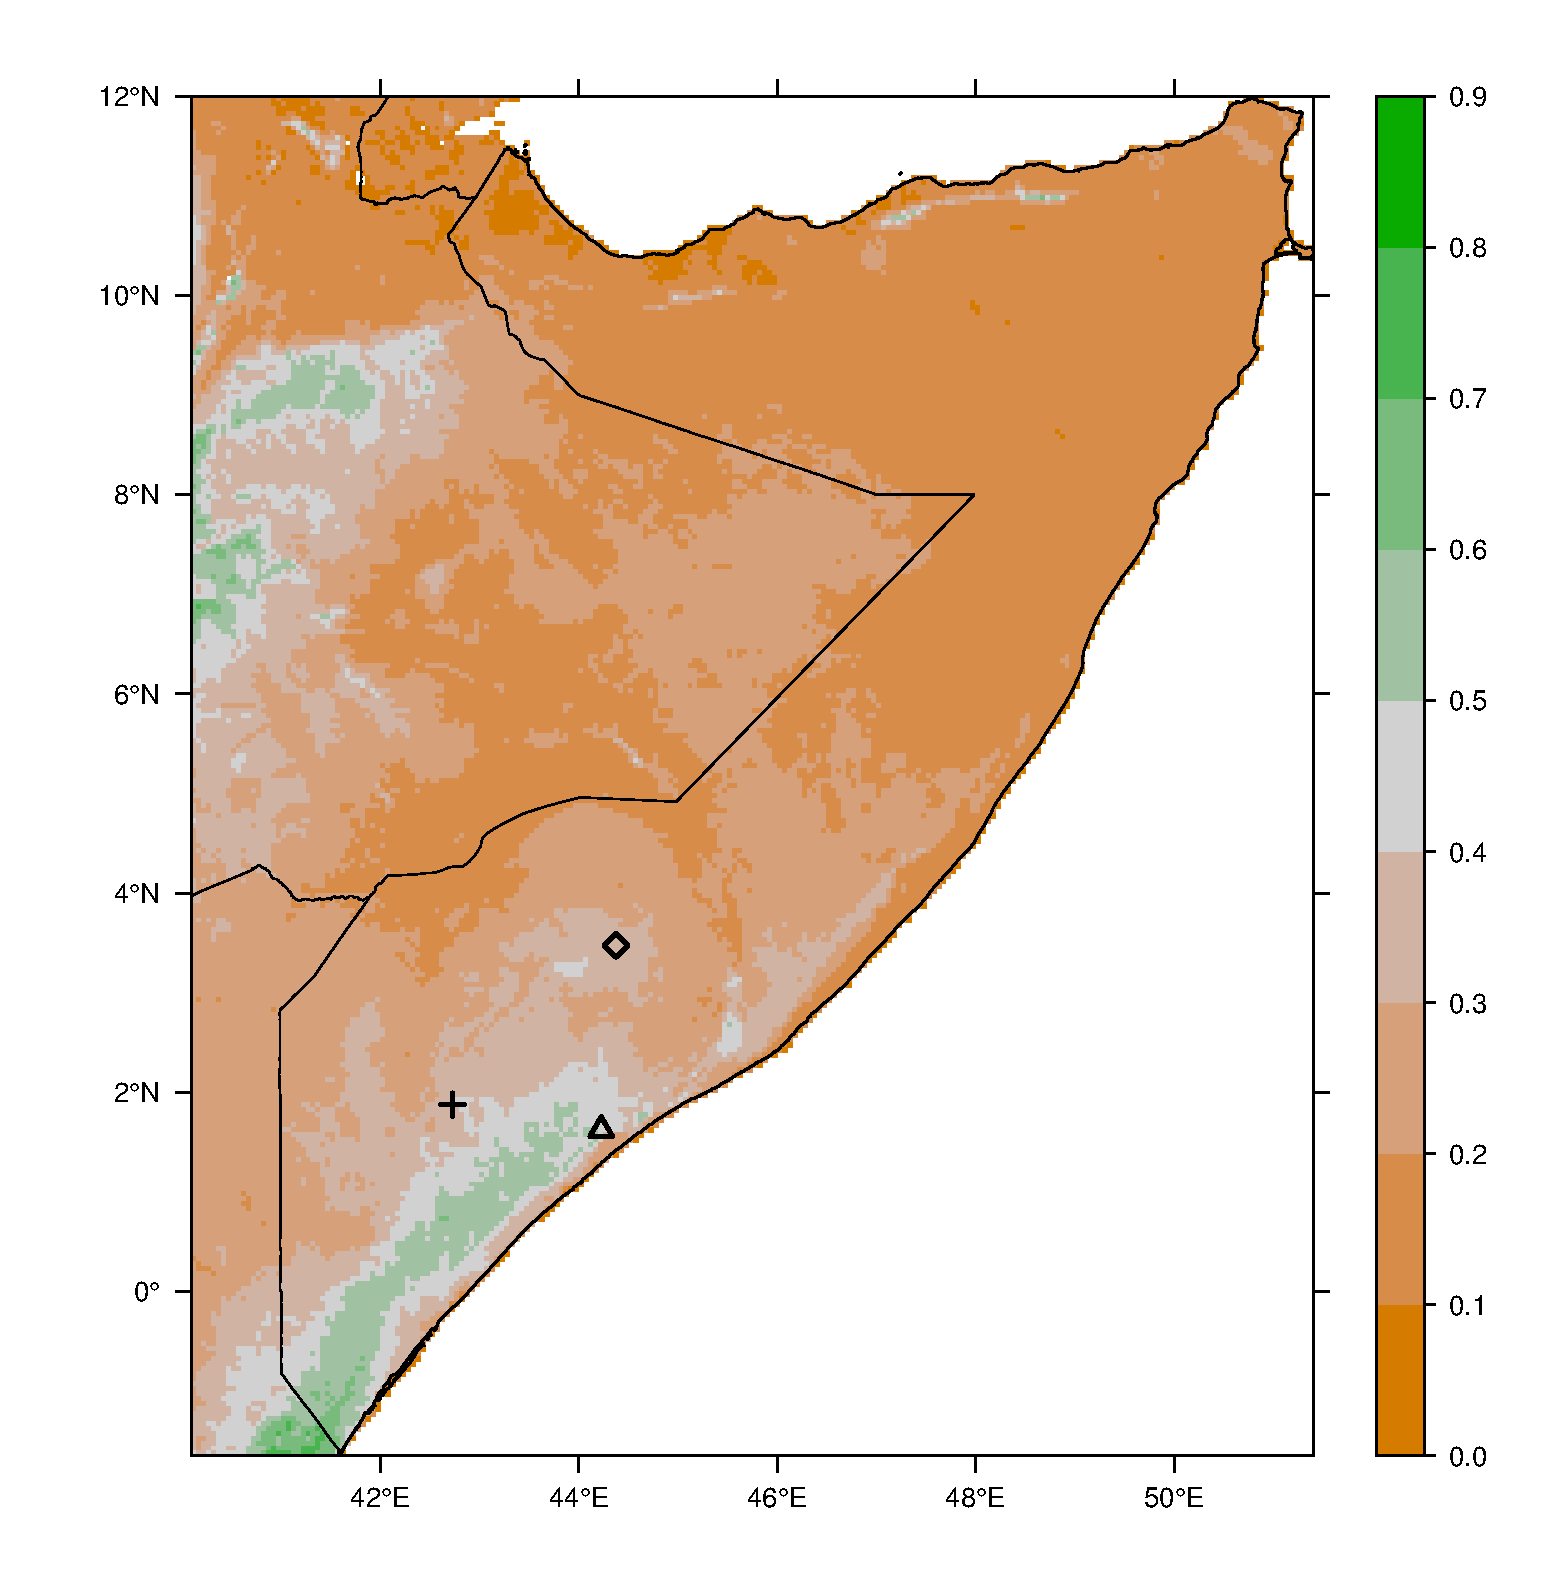
\includegraphics[height=0.7\textwidth]{figs/MedianNDVI_Somalia.png}
%  \caption{Spatial variation of the median 16-day MODIS NDVI image time series from February 2000 until July 2011 covering Somalia as an indicator of average vegetation fractional cover during 2000--2011 period .}
%  \label{fig:MedianNDVI}
%\end{figure}

%%\begin{figure}[htp]
%%\centering
%%    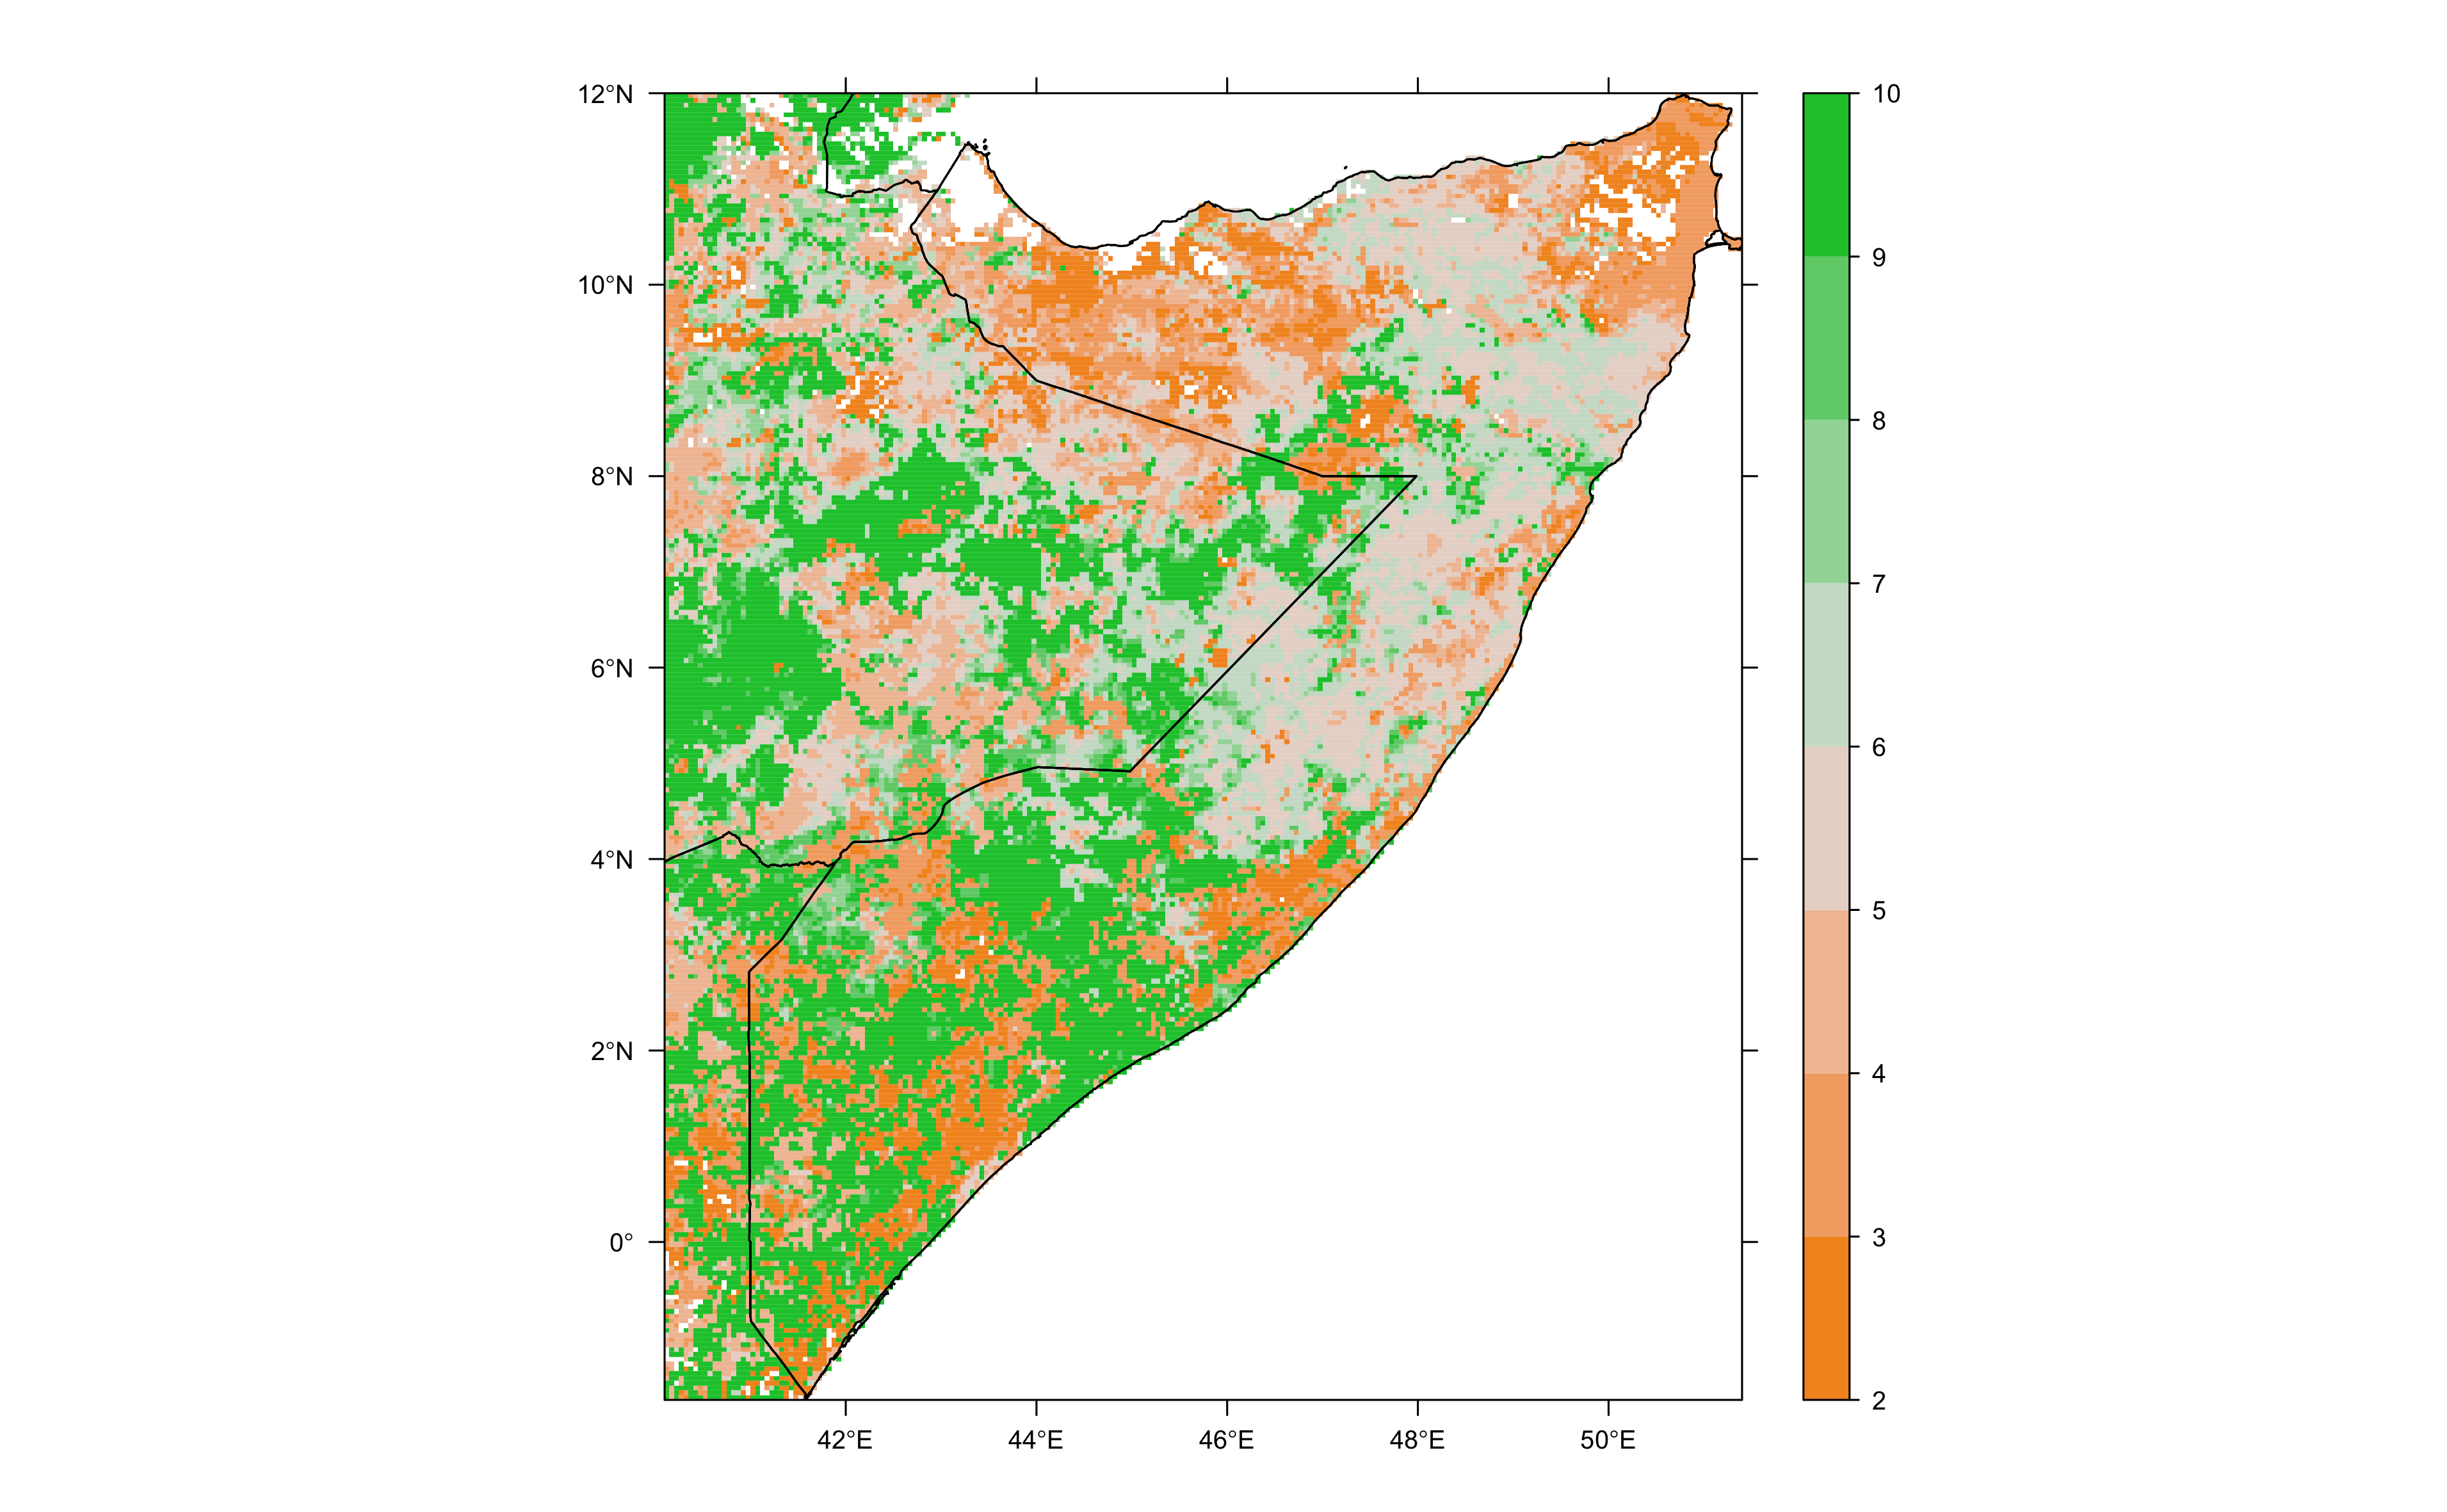
\includegraphics[height=0.7\textwidth]{figs/LengthHistoryPeriod_EA.png}
%%  \caption{Spatial variation of the length the stable history period (expressed in years, i.e., 23 16-day images) within the study area. The length of the history period indicates when in the history period a potential disturbance occurred (e.g., shorter length indicates a more recent disturbance). }
%%  \label{fig:SpatLStableHist}
%%\end{figure}
%%
%%\begin{figure}[htp]
%%\centering
%%    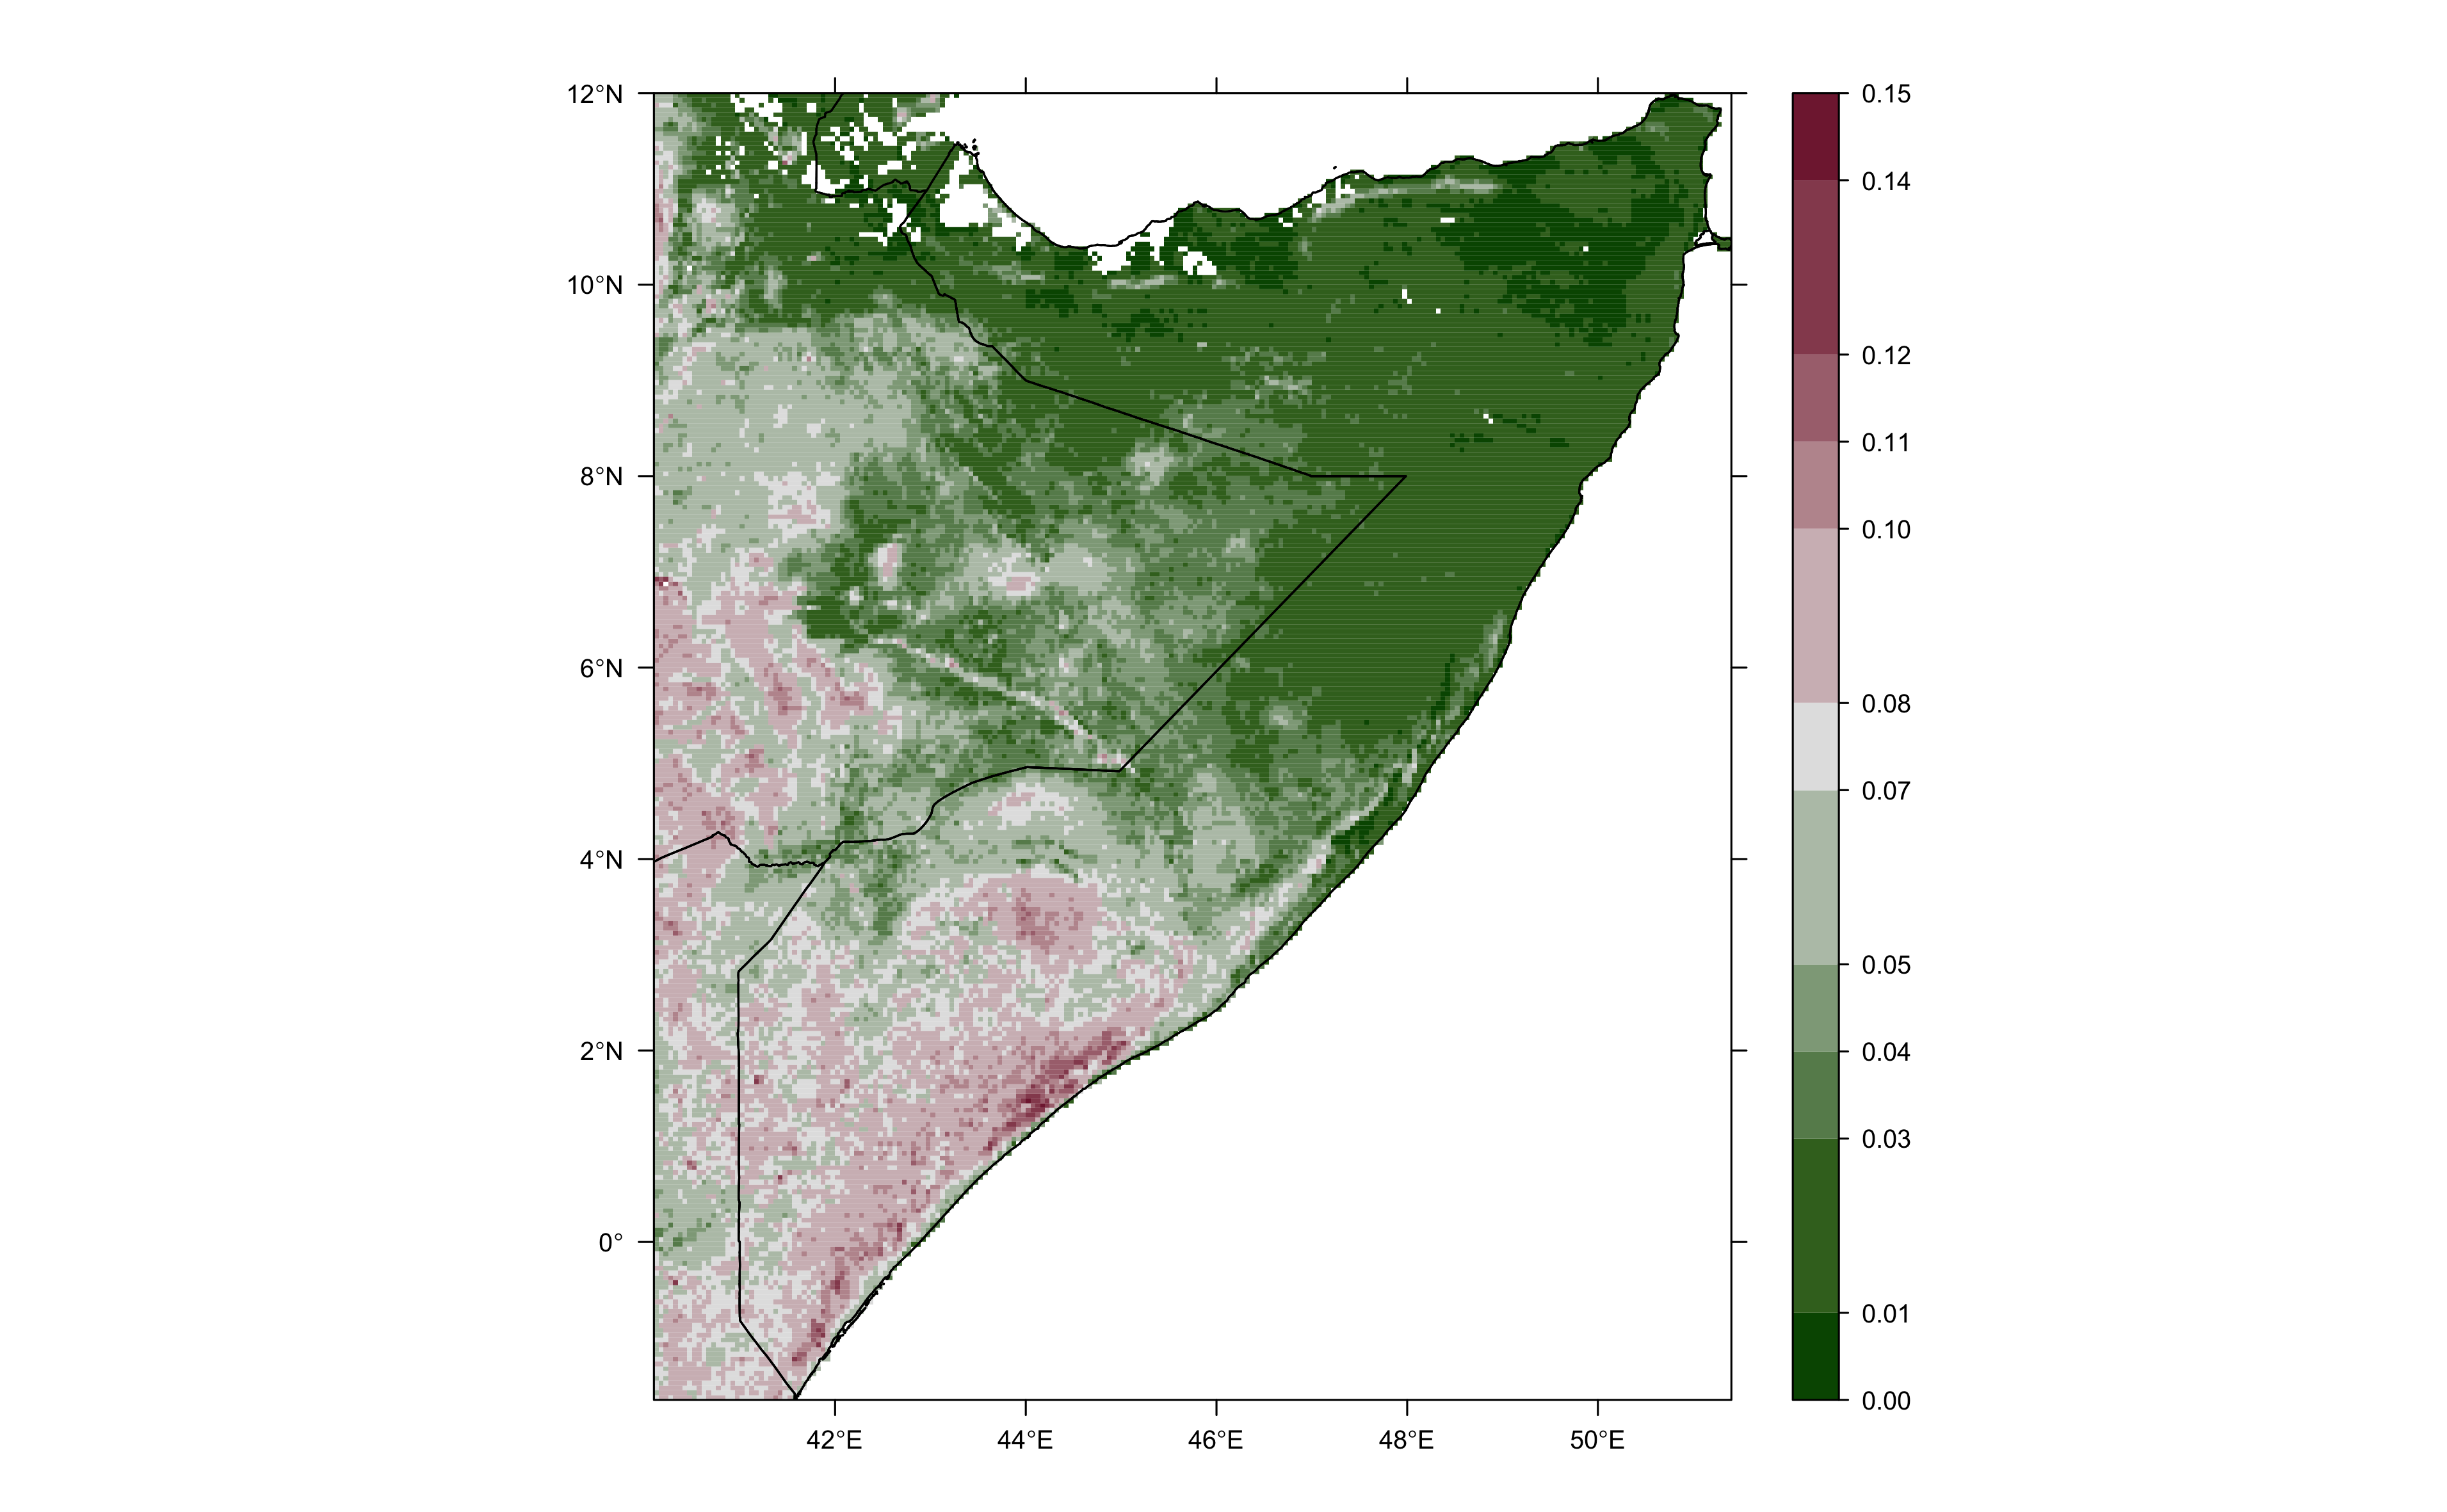
\includegraphics[height=0.7\textwidth]{figs/Noise_EA.png}
%%  \caption{Spatial variation of the noise level (i.e., the standard deviation of the residuals of the stable history model) of Somalia, Eastern Africa. The higher noise levels correspond to the regions with a higher average vegetation cover during the 2000--2011 period as shown in Fig.~\ref{fig:MedianNDVI} refer to simulation results}
%%  \label{fig:SpatNoise}
%%\end{figure}
%%

%\begin{figure}
%\centering
%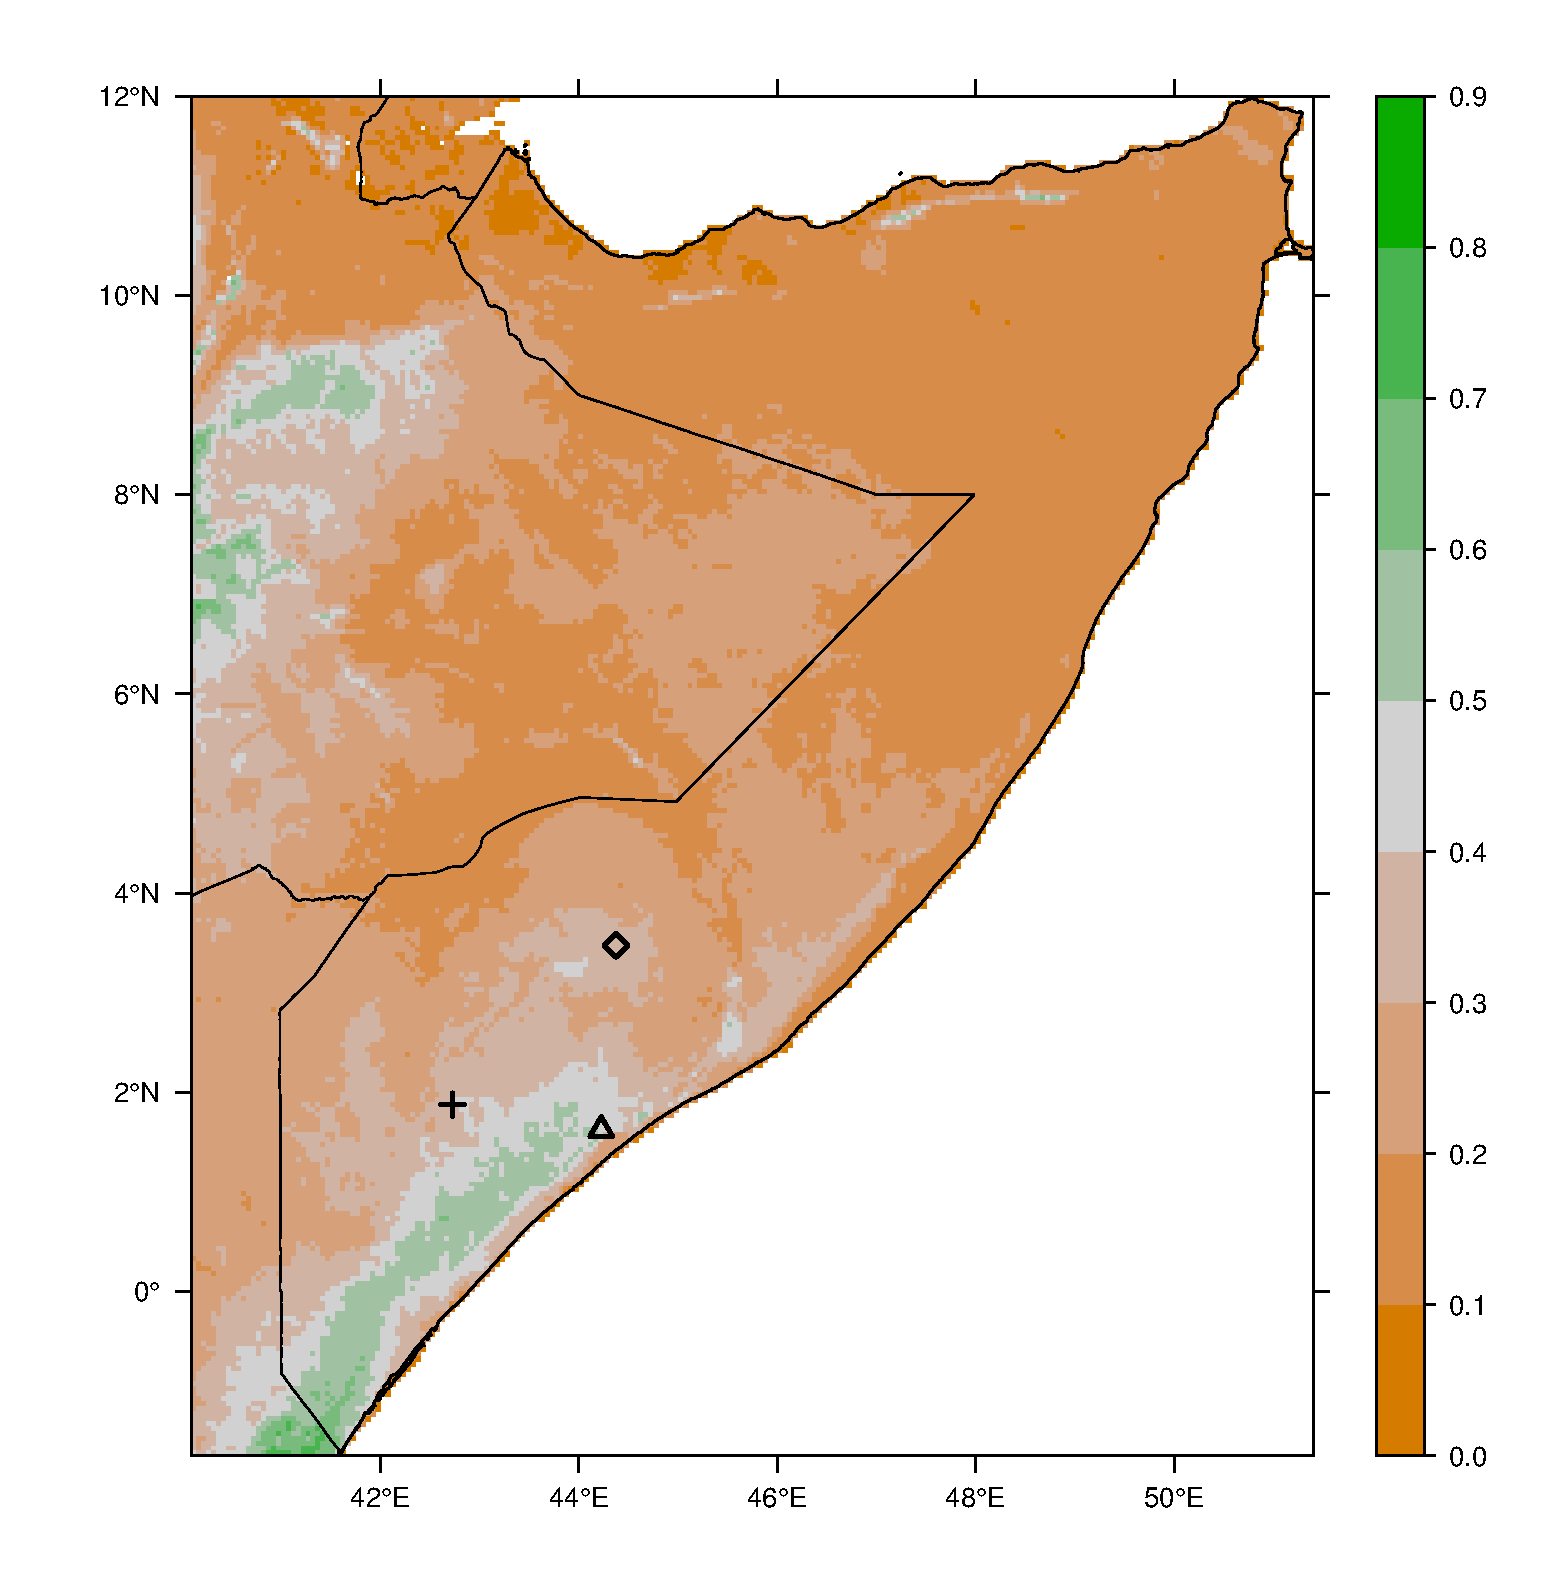
\includegraphics[width=0.5\textwidth]{figs/MedianNDVI_Somalia.png}
% 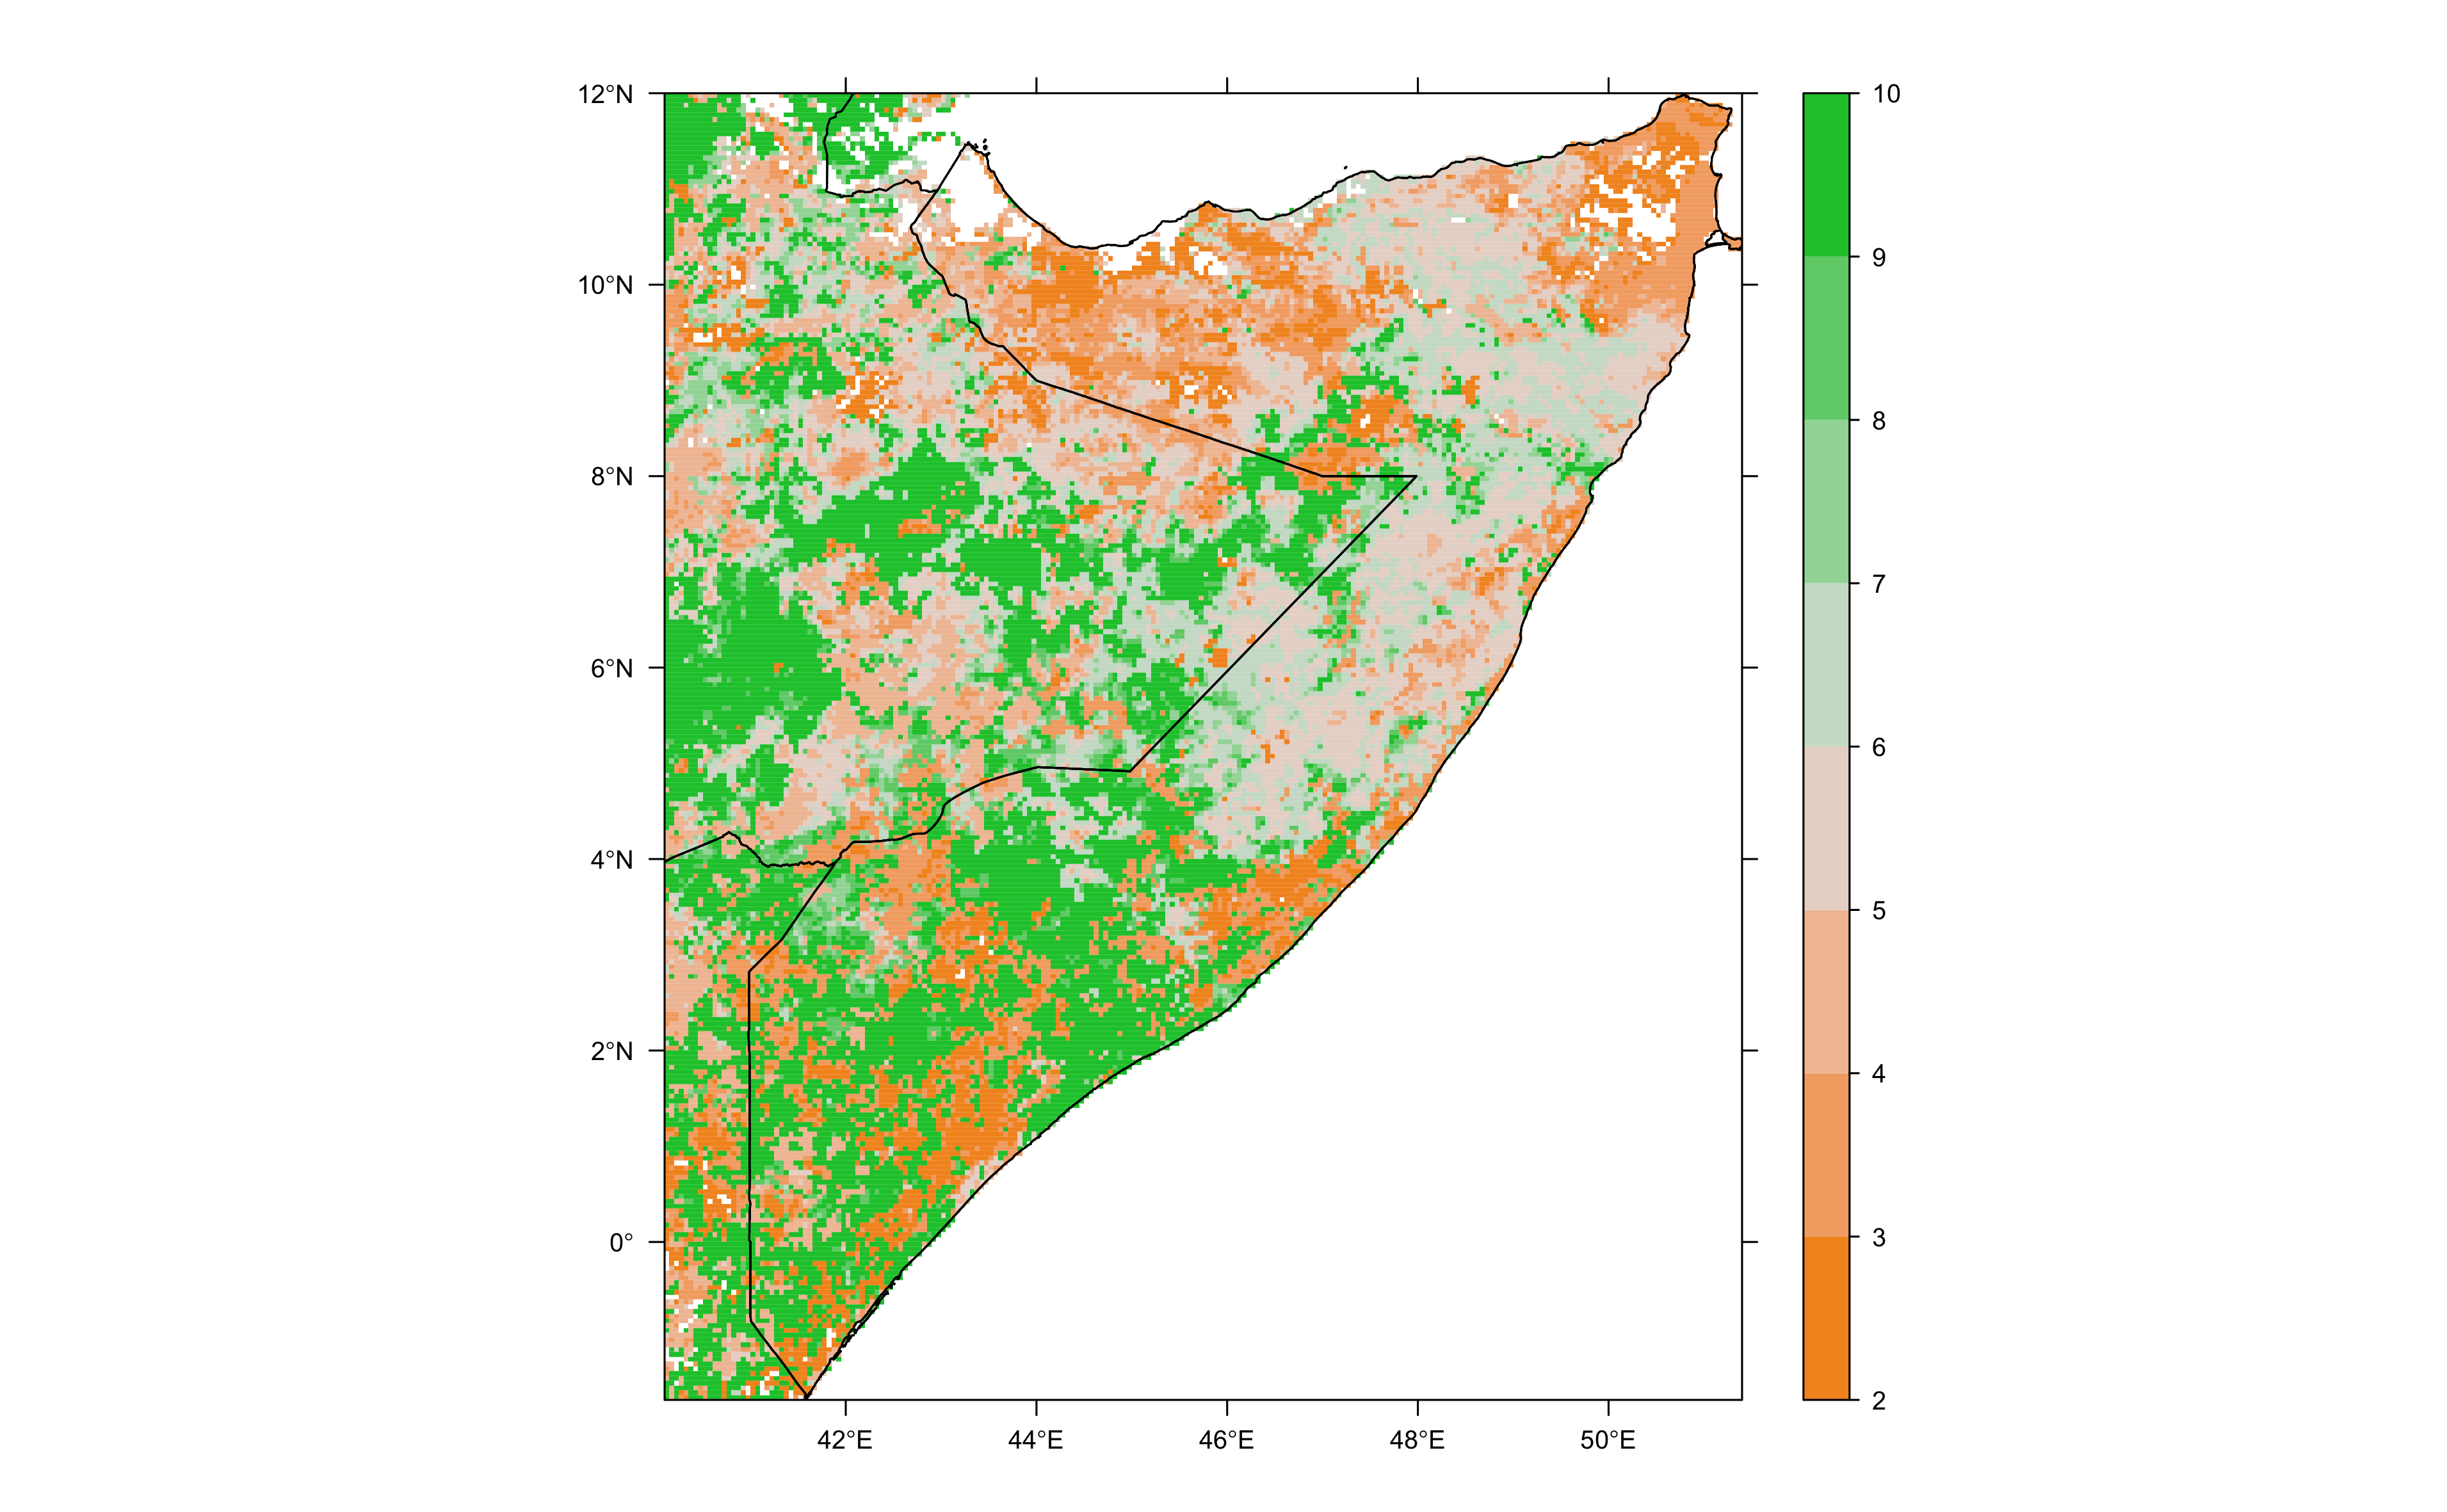
\includegraphics[width=0.5\textwidth]{figs/LengthHistoryPeriod_EA.png}
% \caption{test}
% \label{fig:spatial}
%\end{figure}

%\begin{figure}
%\centering
%\begin{tabular}{cc}
% 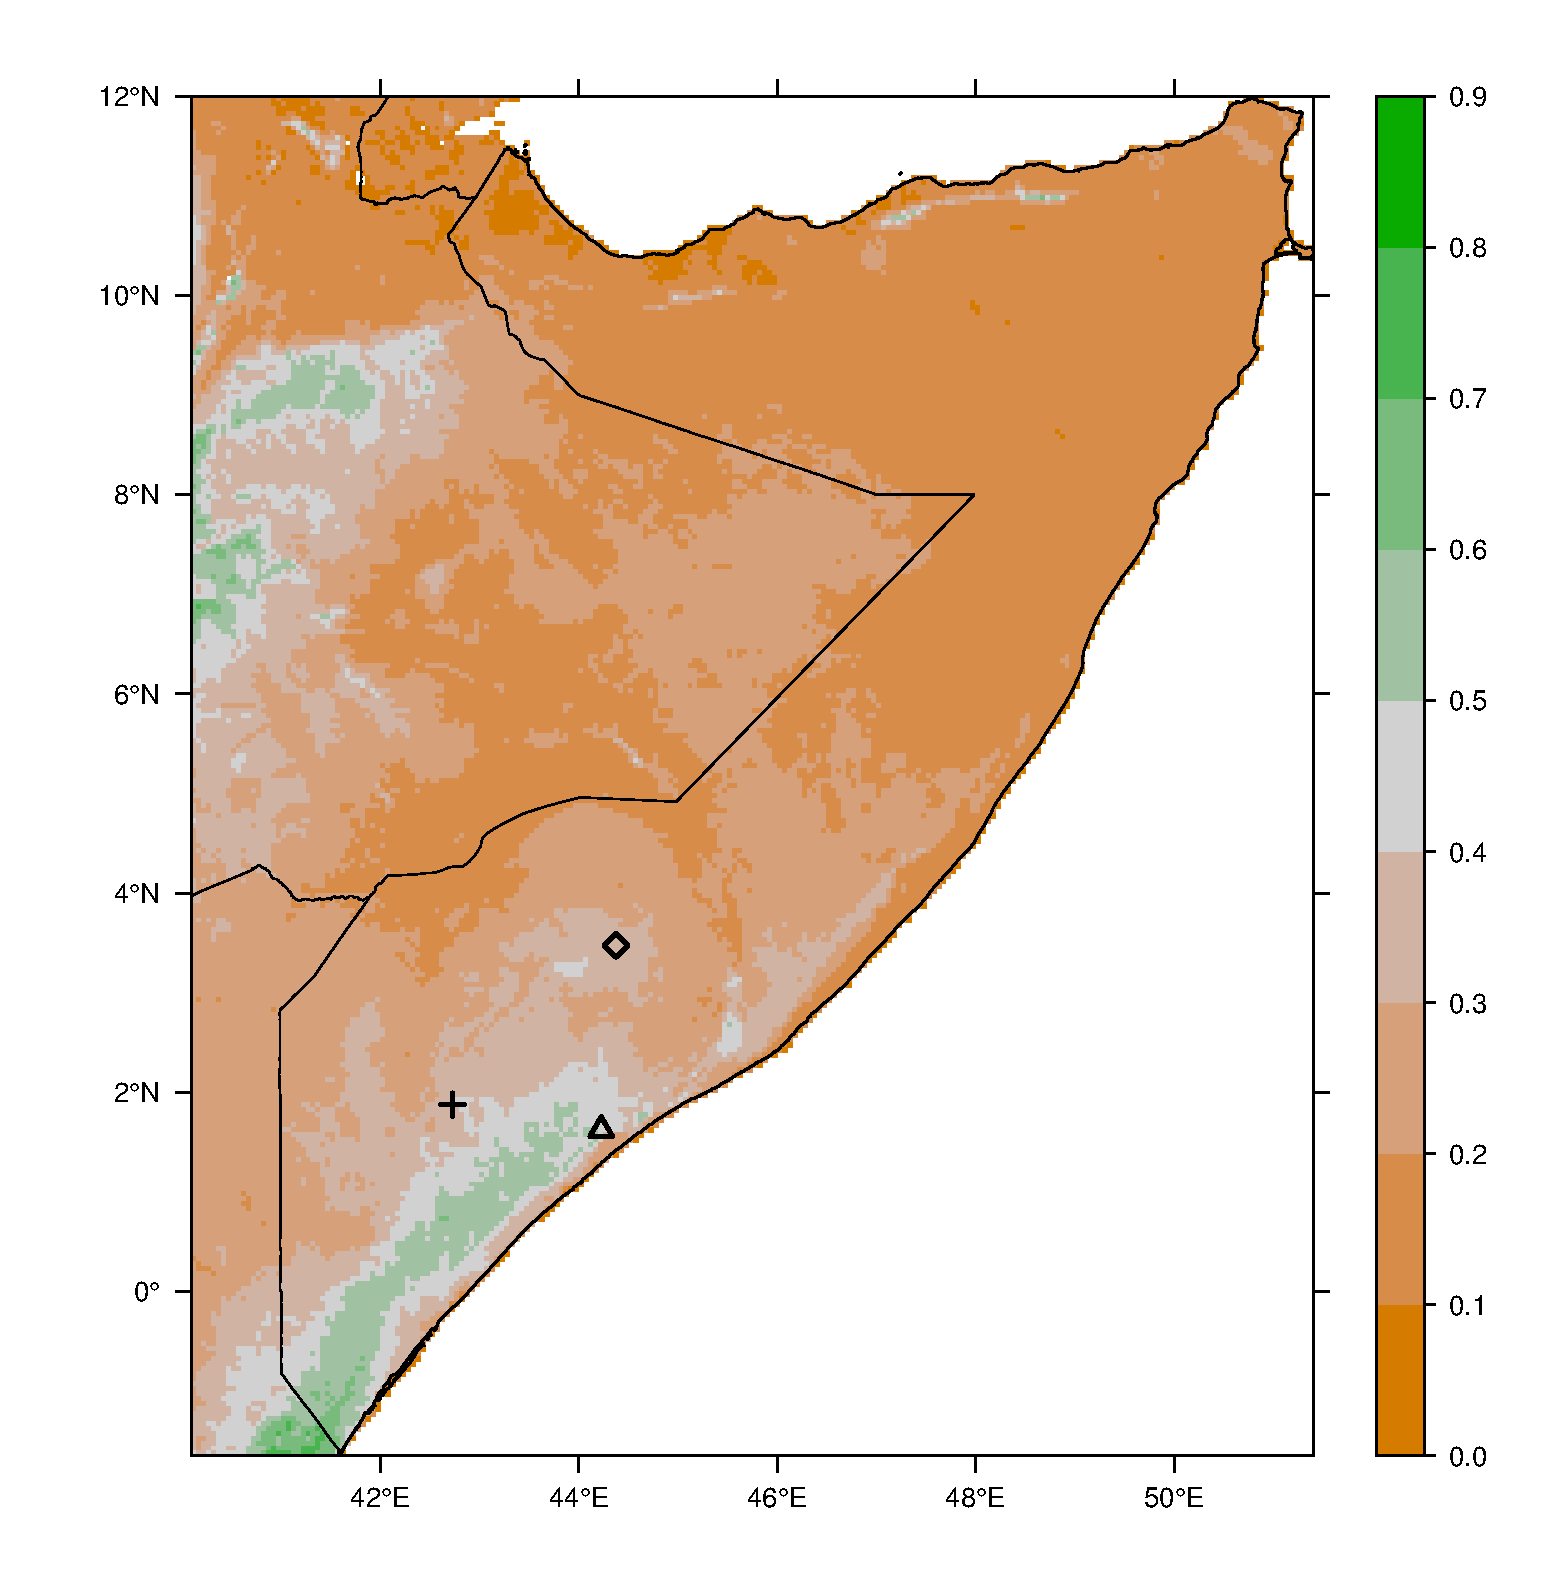
\includegraphics[height=0.5\textwidth,clip=]{figs/MedianNDVI_Somalia.png} &
% 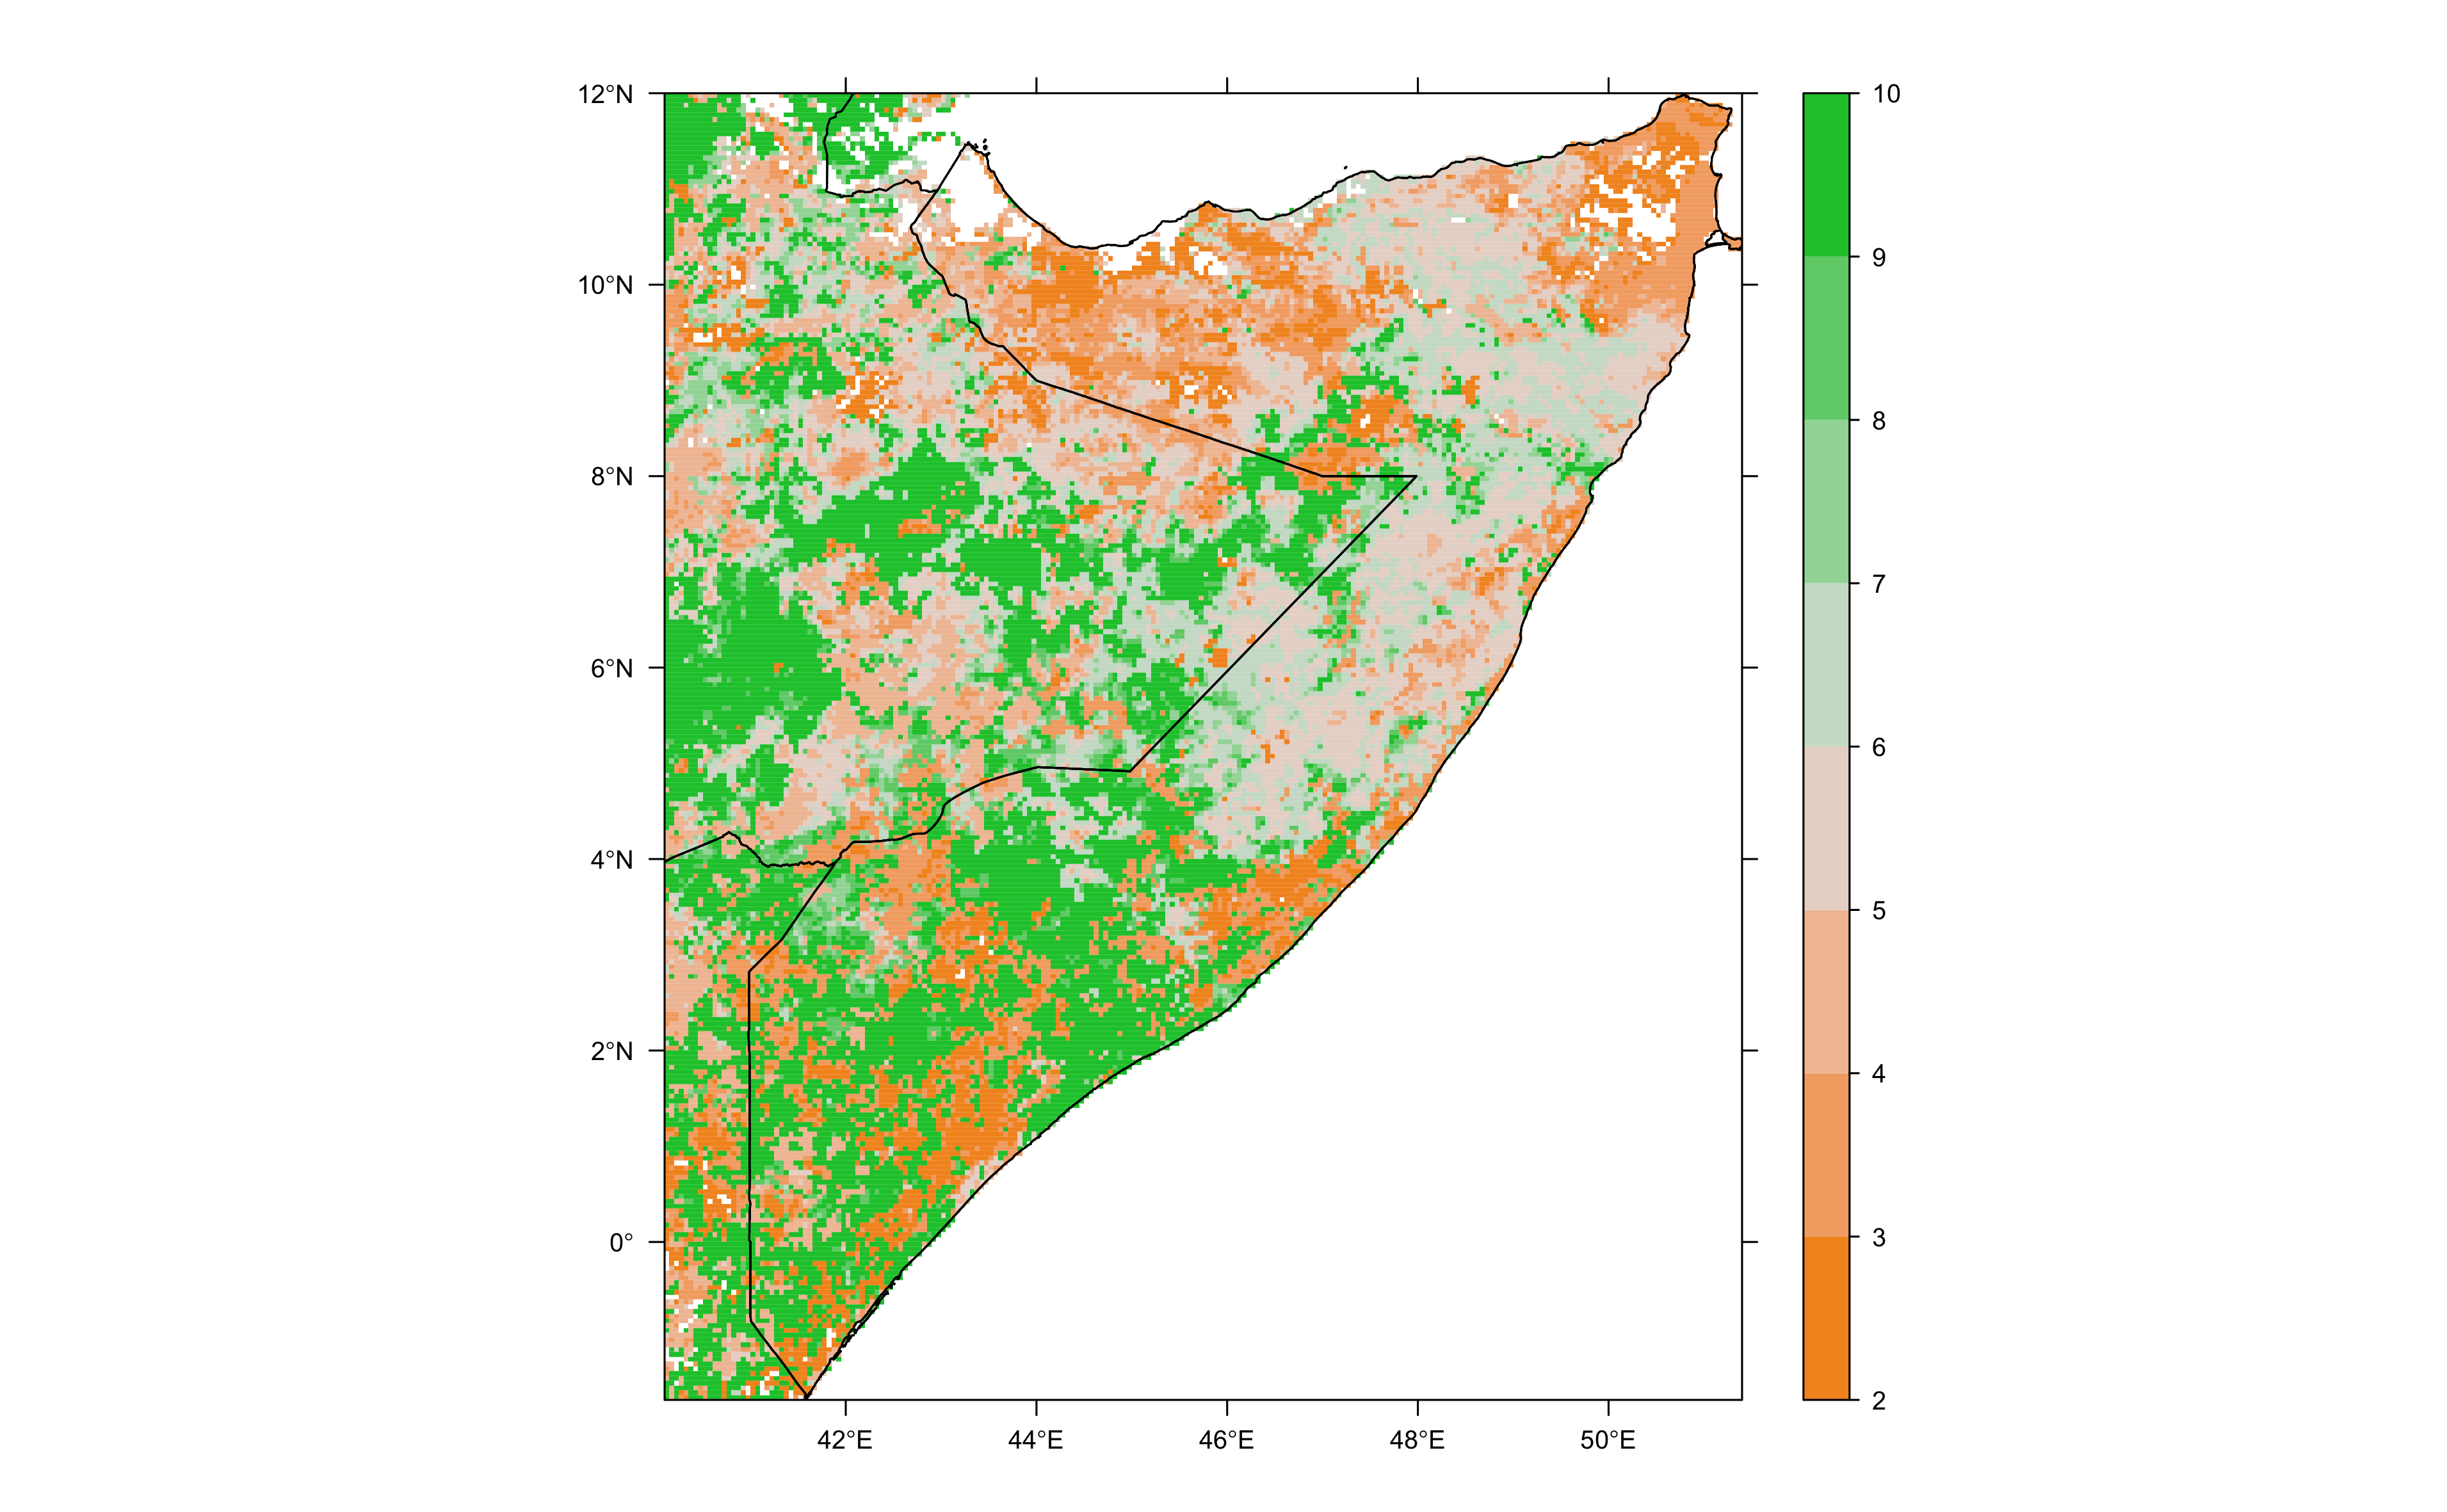
\includegraphics[height=0.5\textwidth,clip=]{figs/LengthHistoryPeriod_EA.png} \\
% 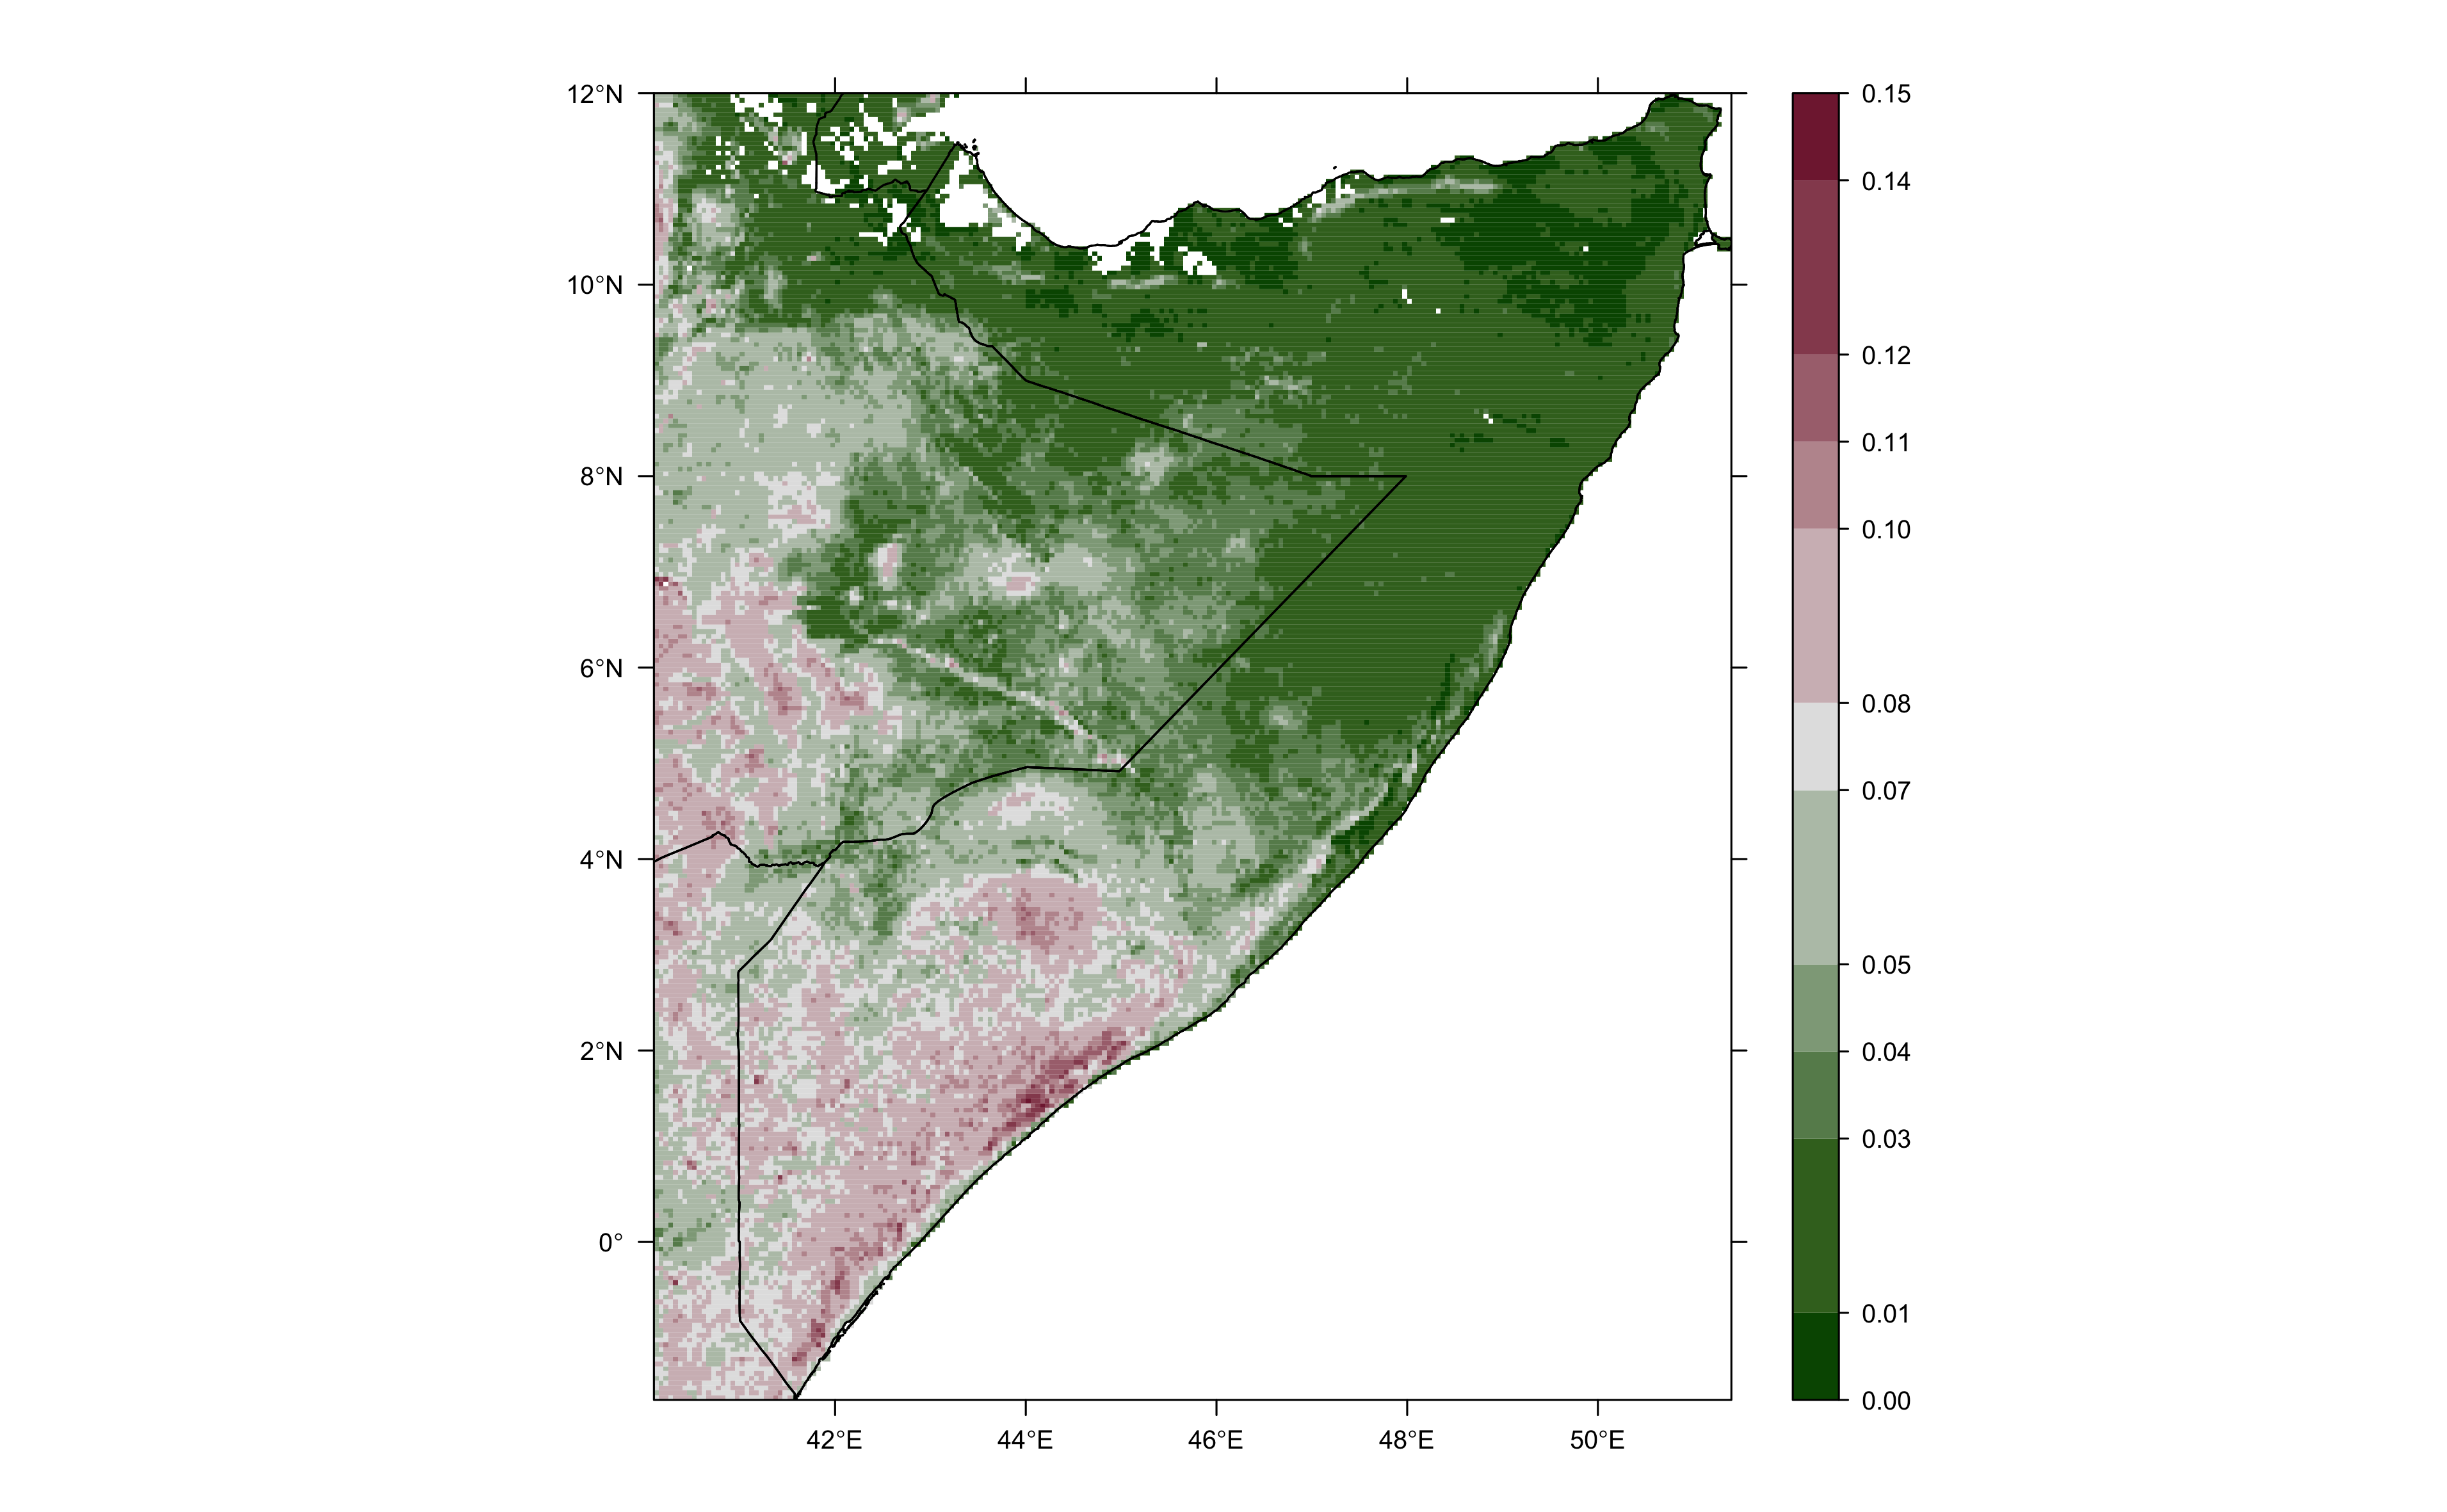
\includegraphics[height=0.5\textwidth,clip=]{figs/Noise_EA.png} &
% 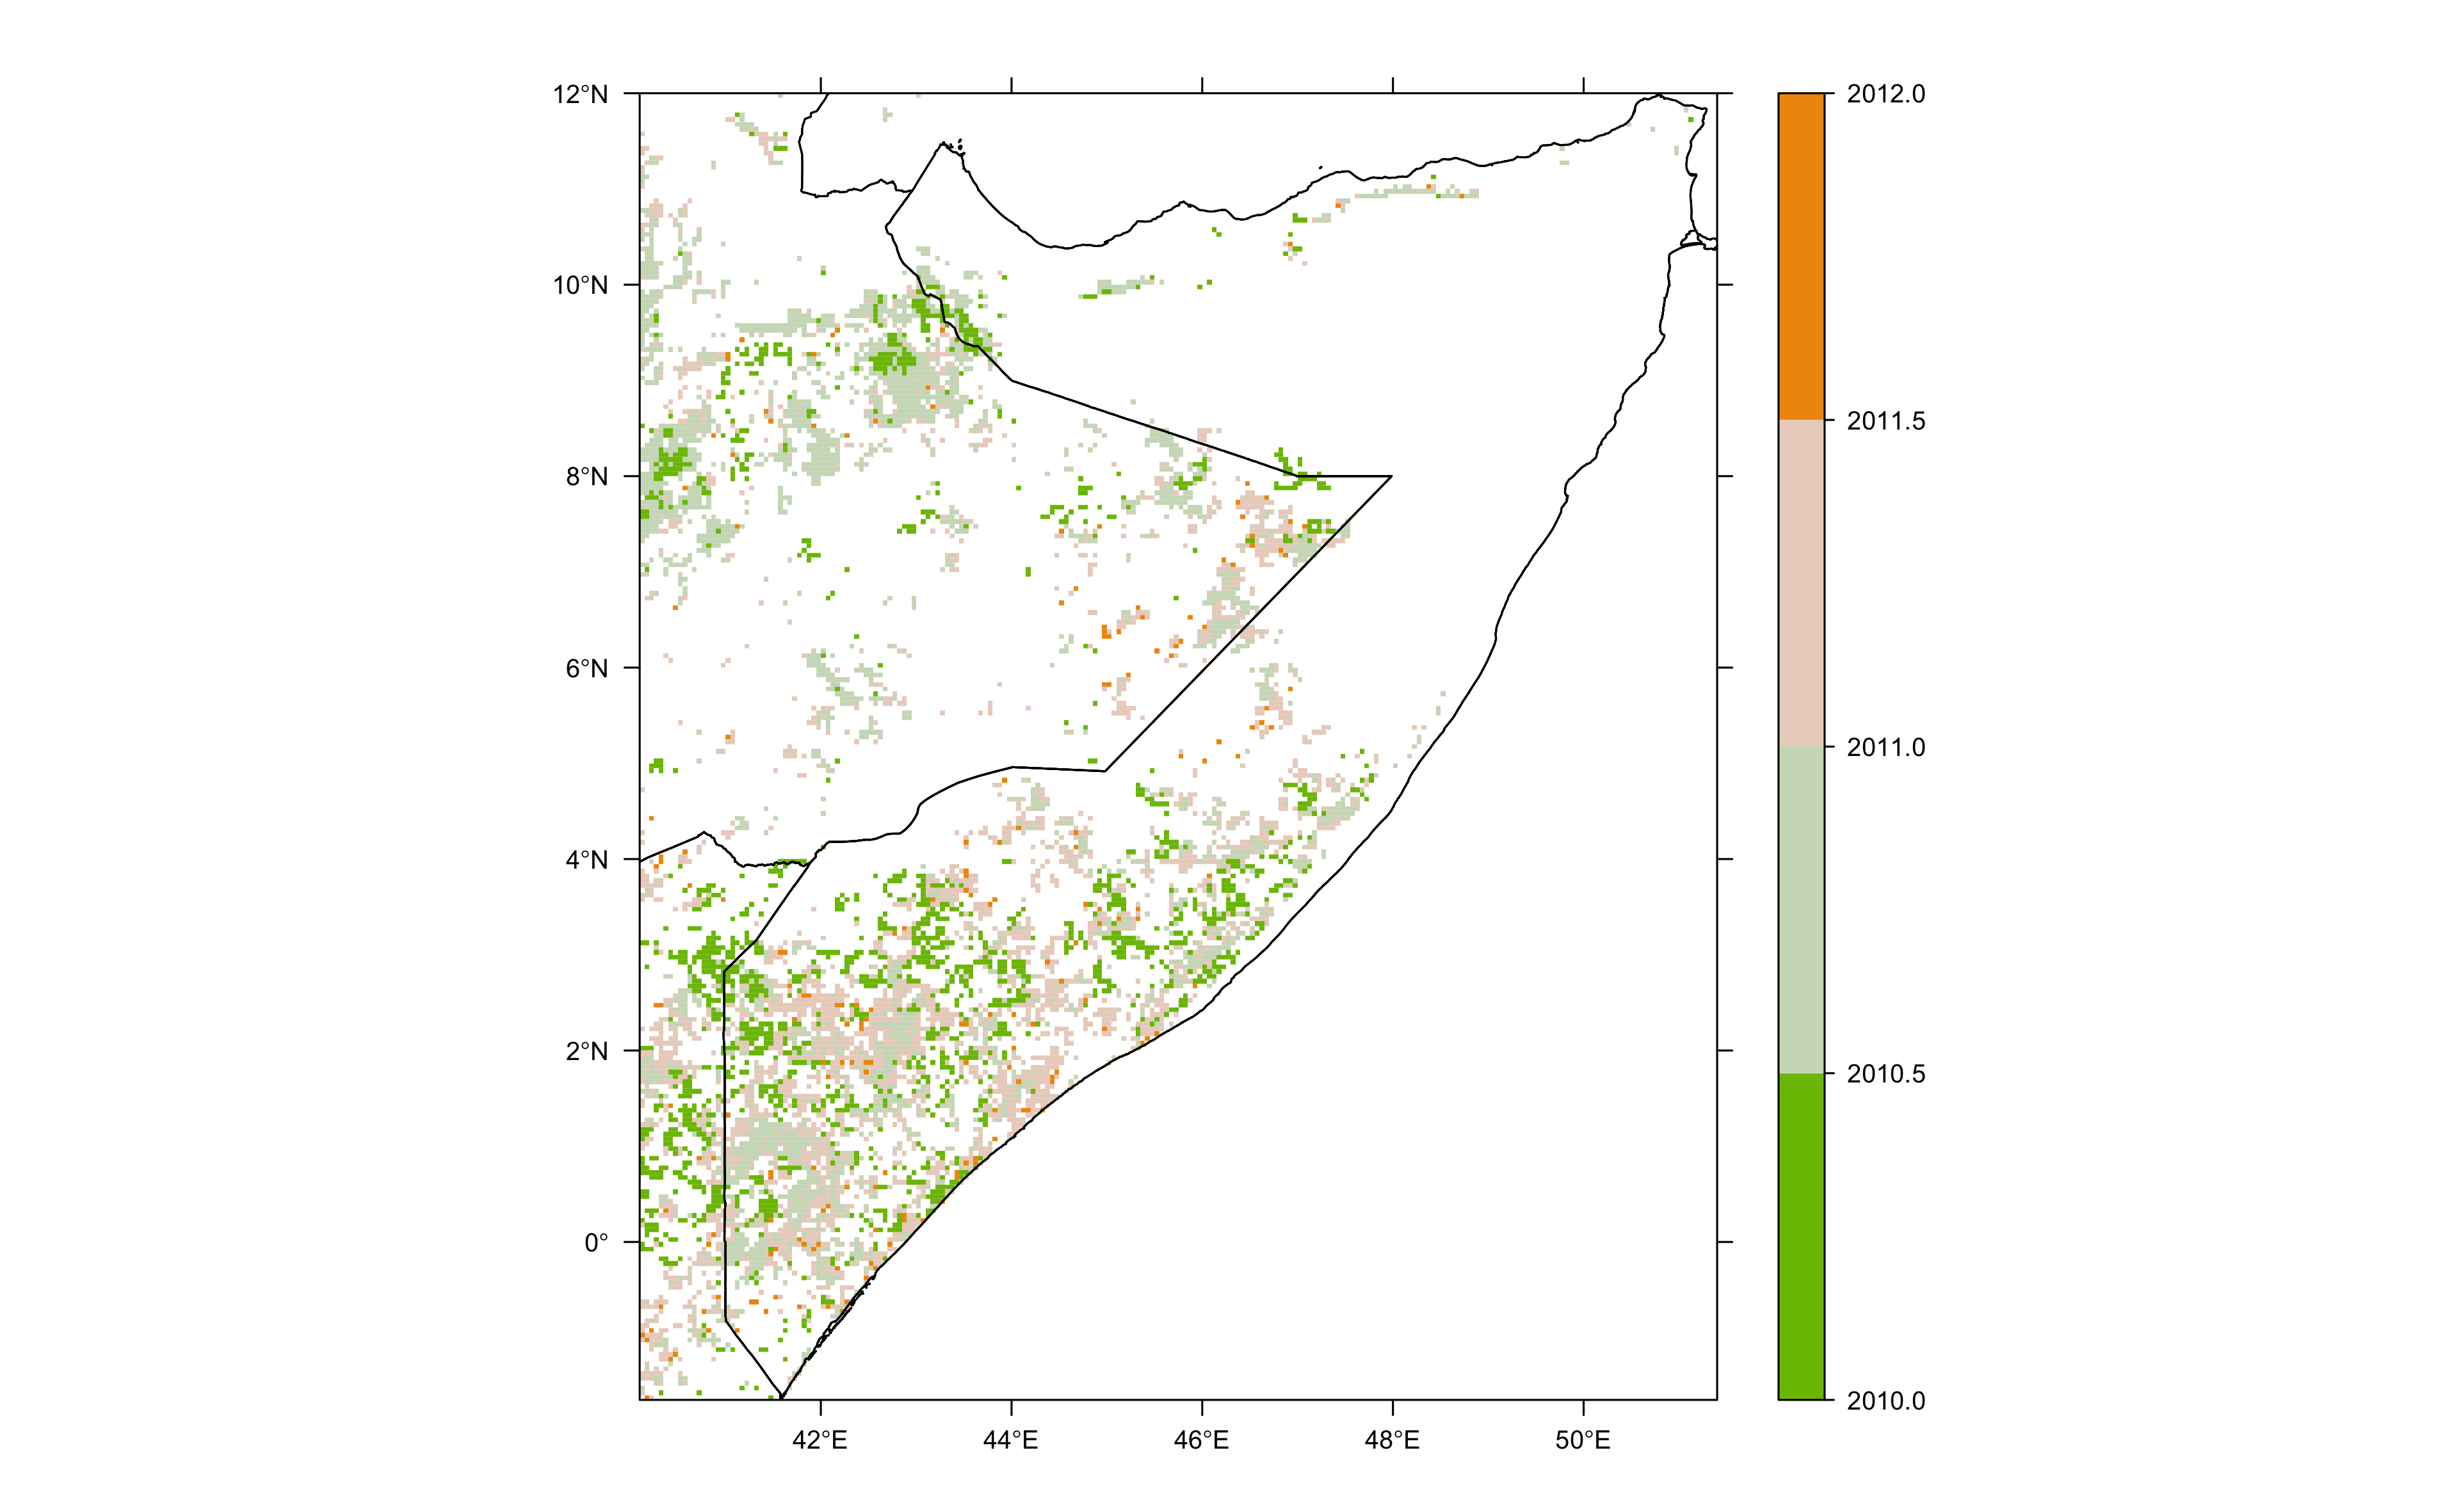
\includegraphics[height=0.5\textwidth,clip=]{figs/TimeofAbnormalBreak_2010_EA} 
%%\epsfig{file=figure1.eps,width=0.5\linewidth,clip=} & 
%%\epsfig{file=figure2.eps,width=0.5\linewidth,clip=} \\
%%\epsfig{file=figure3.eps,width=0.5\linewidth,clip=} &
%%\epsfig{file=figure4.eps,width=0.5\linewidth,clip=}
% \label{fig:spatial}
%\end{tabular}
%\end{figure}

